\RequirePackage[l2tabu,orthodox]{nag}

% TODO: decide if one-sided/two-sided
%\documentclass[headsepline,footsepline,footinclude=false,fontsize=11pt,paper=a4,listof=totoc,bibliography=totoc,BCOR=12mm,DIV=12]{scrbook} % two-sided
\documentclass[headsepline,footsepline,footinclude=false,oneside,fontsize=11pt,paper=a4,listof=totoc,bibliography=totoc]{scrbook} % one-sided

% TODO: change citation style in settings
\PassOptionsToPackage{table,svgnames,dvipsnames}{xcolor}

\usepackage[utf8]{inputenc}
\usepackage[T1]{fontenc}
\usepackage[sc]{mathpazo}
\usepackage[ngerman,american]{babel}
\usepackage[autostyle]{csquotes}
\usepackage[
  backend=biber,
  style=ieee,
  maxnames=99,
  minnames=1,
  giveninits=true
]{biblatex}
\usepackage{graphicx}
\usepackage{scrhack} % necessary for listings package
\usepackage{listings}
\usepackage{lstautogobble}
\usepackage{tikz}
\usepackage{pgfplots}
\usepackage{pgfplotstable}
\usepackage{booktabs}
\usepackage[final]{microtype}
\usepackage{caption}
\usepackage{subcaption}
\usepackage[hidelinks]{hyperref} % hidelinks removes colored boxes around references and links

\bibliography{bibliography}

\setkomafont{disposition}{\normalfont\bfseries} % use serif font for headings
\linespread{1.05} % adjust line spread for mathpazo font

% Add table of contents to PDF bookmarks
\BeforeTOCHead[toc]{{\cleardoublepage\pdfbookmark[0]{\contentsname}{toc}}}

% Define TUM corporate design colors
% Taken from http://portal.mytum.de/corporatedesign/index_print/vorlagen/index_farben
\definecolor{TUMBlue}{HTML}{0065BD}
\definecolor{TUMSecondaryBlue}{HTML}{005293}
\definecolor{TUMSecondaryBlue2}{HTML}{003359}
\definecolor{TUMBlack}{HTML}{000000}
\definecolor{TUMWhite}{HTML}{FFFFFF}
\definecolor{TUMDarkGray}{HTML}{333333}
\definecolor{TUMGray}{HTML}{808080}
\definecolor{TUMLightGray}{HTML}{CCCCC6}
\definecolor{TUMAccentGray}{HTML}{DAD7CB}
\definecolor{TUMAccentOrange}{HTML}{E37222}
\definecolor{TUMAccentGreen}{HTML}{A2AD00}
\definecolor{TUMAccentLightBlue}{HTML}{98C6EA}
\definecolor{TUMAccentBlue}{HTML}{64A0C8}

% Settings for pgfplots
\pgfplotsset{compat=newest}
\pgfplotsset{
  % For available color names, see http://www.latextemplates.com/svgnames-colors
  cycle list={TUMBlue\\TUMAccentOrange\\TUMAccentGreen\\TUMSecondaryBlue2\\TUMDarkGray\\},
}

% Settings for lstlistings
\lstset{%
  basicstyle=\ttfamily,
  columns=fullflexible,
  autogobble,
  keywordstyle=\bfseries\color{TUMBlue},
  stringstyle=\color{TUMAccentGreen}
}


% TODO: change thesis information
\newcommand*{\getUniversity}{Technische Universität München}
\newcommand*{\getFaculty}{Department of Informatics}
\newcommand*{\getTitle}{Enhancing a Visualization Concept for Environmental Perception Data
of Autonomous Vehicles}
\newcommand*{\getTitleGer}{Weiterentwicklung eines Visualisierungskonzepts für Umweltwahrnehmungsdaten von Autonome Fahrzeuge}
\newcommand*{\getAuthor}{Tarik Isildar}
\newcommand*{\getDoctype}{Master's Thesis in Informatics}
\newcommand*{\getSupervisor}{Prof. Dr.-Ing. Markus Lienkamp}
\newcommand*{\getAdvisor}{Tobias Kerbl, M.Sc.}
\newcommand*{\getSubmissionDate}{Submission date}
\newcommand*{\getSubmissionLocation}{Munich}

\begin{document}

% Set page numbering to avoid "destination with the same identifier has been already used" warning for cover page.
% (see https://en.wikibooks.org/wiki/LaTeX/Hyperlinks#Problems_with_Links_and_Pages).
\pagenumbering{alph}
\begin{titlepage}
  % HACK for two-sided documents: ignore binding correction for cover page.
  % Adapted from Markus Kohm's KOMA-Script titlepage=firstiscover handling.
  % See http://mirrors.ctan.org/macros/latex/contrib/koma-script/scrkernel-title.dtx,
  % \maketitle macro.
  \oddsidemargin=\evensidemargin\relax
  \textwidth=\dimexpr\paperwidth-2\evensidemargin-2in\relax
  \hsize=\textwidth\relax

  \centering

  \IfFileExists{logos/tum.pdf}{%
    \includegraphics[height=20mm]{logos/tum.pdf}
  }{%
    \vspace*{20mm}
  }

  \vspace{5mm}
  {\huge\MakeUppercase{\getFaculty{}}}\\

  \vspace{5mm}
  {\large\MakeUppercase{\getUniversity{}}}\\

  \vspace{20mm}
  {\Large \getDoctype{}}

  \vspace{15mm}
  {\huge\bfseries \getTitle{}}

  \vspace{15mm}
  {\LARGE \getAuthor{}}

  \IfFileExists{logos/faculty.pdf}{%
    \vfill{}
    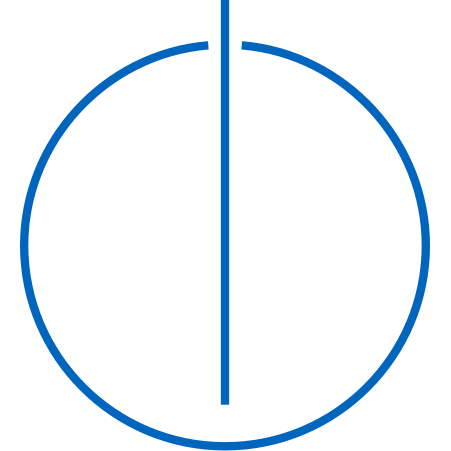
\includegraphics[height=20mm]{logos/faculty.pdf}
  }{}
\end{titlepage}


\frontmatter{}

\begin{titlepage}
  \centering

  \IfFileExists{logos/tum.pdf}{%
    \includegraphics[height=20mm]{logos/tum.pdf}
  }{%
    \vspace*{20mm}
  }

  \vspace{15mm}
  {\huge\MakeUppercase{\getFaculty{}}}\\

  \vspace{5mm}
  {\large\MakeUppercase{\getUniversity{}}}\\

  \vspace{15mm}
  {\Large \getDoctype{}}

  \vspace{10mm}
  {\huge\bfseries \getTitle{} \par}


  \vspace{5mm}
  {\huge\bfseries \foreignlanguage{ngerman}{\getTitleGer{}} \par}

  \vspace{15mm}
  \begin{tabular}{l l}
    Author:          & \getAuthor{} \\
    Supervisor:      & \getSupervisor{} \\
    Advisor:         & \getAdvisor{} \\
    Submission Date: & \getSubmissionDate{} \\
  \end{tabular}


  \IfFileExists{logos/faculty.pdf}{%
    \vfill{}
    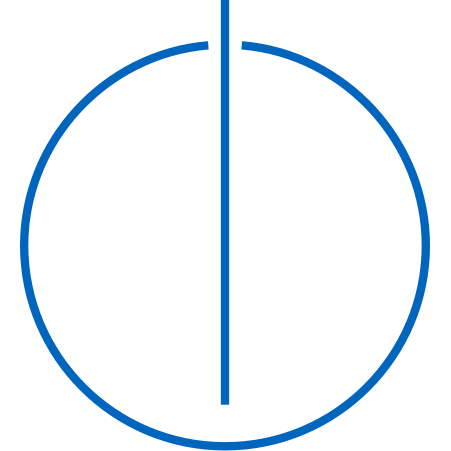
\includegraphics[height=20mm]{logos/faculty.png}
  }{}
\end{titlepage}

\thispagestyle{empty}
\vspace*{0.8\textheight}
\noindent
I confirm that this \MakeLowercase{\getDoctype{}} is my own work and I have documented all sources and material used.

\vspace{15mm}
\noindent
\getSubmissionLocation{}, \getSubmissionDate{} \hspace{50mm} \getAuthor{}

\cleardoublepage{}

\addcontentsline{toc}{chapter}{Acknowledgments}
\thispagestyle{empty}

\vspace*{20mm}

\begin{center}
{\usekomafont{section} Acknowledgments}
\end{center}

\vspace{10mm}

%TODO: Acknowledgments

\cleardoublepage{}


\chapter{List of Abbreviations}
\begin{acronym}
    \acro{AV}{Autonomous Vehicle}
    \acrodefplural{AV}[AVs]{Autonomous Vehicles}
    \acro{HMI}{Human-Machine Interface}
    \acrodefplural{HMI}[HMIs]{Human-Machine Interfaces}
    \acro{SAGAT}{Situation Awareness Global Assessment Technique}
    \acro{SART}{Situation Awareness Rating Technique}
    \acro{SAE}{Society of Automotive Engineers}
    \acro{NASA-TLX}{NASA Task Load Index}
    \acro{SA}{Situational Awareness}
    \acro{AD}{Autonomous Driving}
    \acro{PM}{Perception Modification}
    \acro{ODD}{Operational Design Domain}
    \acro{NeRF}{Neural Radiance Fields}
    \acro{KPI}{Key Performance Indicator}
    \acrodefplural{KPI}[KPIs]{Key Performance Indicators}
    \acro{GUI}{Graphical User Interface}
    \acrodefplural{GUI}[GUIs]{Graphical User Interfaces}
    \acro{AI}{Artificial Intelligence}
    \acro{DL}{Deep Learning}
    \acro{CSPN}{Convolutional Spatial Propagation Network}
    \acro{DySPN}{Dynamic Spatial Propagation Network}
    \acro{SLAM}{Simultaneous Localization and Mapping}
    \acro{LiDAR}{Light Detection and Ranging}
    \acro{GPS}{Global Positioning System}
    \acro{IMU}{Inertial Measurement Unit}
    \acro{iRMSE}{Inverse Root Mean Squared Error}
    \acro{iMAE}{Inverse Mean Absolute Error}
    \acro{MAE}{Mean Absolute Error}
    \acro{FOV}{Field of View}
    \acro{SSIM}{Structural Similarity Index Measure}
\end{acronym}

%TODO: Abbreviations

\cleardoublepage{}



\chapter{\abstractname}

%TODO: Abstract

    Teleoperation serves as a crucial backup system for \acp{AV}, enabling human operators to assist when situations exceed the vehicle's capabilities. This thesis focuses on \ac{PM}, a teleoperation approach that allows operators to correct perception errors without taking full control of the vehicle. The research develops and evaluates a new interface design to improve how operators interact with sensor data during these correction tasks.

    The main contribution is the development of an Integrated View interface that combines camera feeds, LiDAR data, and perception outputs in a single display. This implementation uses a \ac{DL} based depth completion model to create detailed 3D visualizations from sparse sensor data, enabling real-time operation. For comparison, we also developed a traditional Separate View interface that presents information across multiple windows.

    To evaluate these interfaces, we created a structured testing framework using established metrics: \ac{SAGAT} for measuring operator awareness and \ac{NASA-TLX} for assessing cognitive workload. The study environment features a custom simulation based on Munich's road layout, ensuring realistic testing conditions for German operators.

While comprehensive user testing is still ongoing, initial technical assessments suggest that combining multiple data streams into a single view could simplify operator decision-making during Perception Modification tasks. The research demonstrates the feasibility of real-time depth completion in teleoperation systems and establishes a foundation for future interface improvements. These findings contribute to the development of more effective teleoperation systems, strengthening the role of human oversight in \ac{AV} operations.

\microtypesetup{protrusion=false}
\tableofcontents{}
\microtypesetup{protrusion=true}

\mainmatter{}

% !TeX root = ../main.tex
% Add the above to each chapter to make compiling the PDF easier in some editors.

\chapter{Introduction}\label{chapter:introduction}

Autonomous Driving (AD) has been a topic of intense interest for researchers and
industry professionals for the past few decades. Despite significant investments and
efforts that we can see recently in the funding of Waymo \cite{waymo2024funding}, Wayve \cite{wayve2024funding},
and numerous others, public acceptance remains a challenge. A Forbes Advisor
survey \cite{forbes2024} conducted in January 2024 revealed that 93\% of the population harbors
concerns about self-driving cars, with safety and technology malfunctions topping the
list of worries
This widespread apprehension underscores the need for robust systems

In light of these challenges, teleoperation has emerged as a crucial component
in developing and deploying autonomous vehicles. Teleoperation allows
human operators to remotely assist or take control of autonomous vehicles when they
encounter situations beyond their current capabilities. Research by Kettwich et al. \cite{Kettwich}
emphasizes the importance of effective Human-Machine Interfaces (HMI) in
teleoperation, showing that well-designed interfaces can significantly improve user
acceptance and usability of autonomous systems.

Among various teleoperation concepts, this thesis focuses specifically on Perception Modification \cite{Feiler2021ThePM},
ranked as the most effective approach for
addressing common autonomous vehicle failure cases \cite{Brecht} .The effectiveness of
teleoperation, especially in Perception Modification, heavily relies on the quality of the HMI used by operators.

This thesis compares two interface designs for teleoperation: the 'Separate View,'
which presents 2D camera feeds and 3D perception data on separate displays, and
the 'Integrated View,' which combines all raw sensor data and perception data in a single window.
(For detailed descriptions of these interfaces, see sections \ref{section:separateview} and \ref{section:integratedview}).

In a recent study by Prinz et al.\cite{vizualizationUserStudy}, it was demonstrated that utilizing a 2D video stream for teleoperating a robotic arm
significantly increases the mission completion time due to reduced operator performance. To address this limitation,
we propose the use of a novel Integrated View interface, that aims to provide operators a more comprehensive understanding of the environment.
By enhancing situational awareness and improving decision-making capabilities, particularly in complex environments, we believe this approach
will mitigate the performance loss for the remote teleoperation.

\section{Objective}
The primary objective of this thesis is to develop and evaluate an advanced Human-Machine Interface (HMI) for the teleoperation of autonomous vehicles, with a specific focus on enhancing situational awareness for Perception Modification tasks. To achieve this, we aim to Design and implement an "Integrated View" interface that combines all raw sensor data and perception data - what we call "Environmental Data" - in a single window, providing operators with a comprehensive and cohesive view of the vehicle's environment. The main objectives of this thesis can be summarized as follows:
\begin{itemize}
    \item Compare the effectiveness of the 'Integrated View' interface, which provides a comprehensive view of the vehicle's environment, against a traditional 'Separate View' interface through a rigorous user study.
    \item Evaluate the impact of the 'Integrated View' and 'Separate View' interfaces on operator situational awareness is conducted with the scientific rigor of the Situation Awareness Global Assessment Technique (SAGAT) \cite{endsley1988sagat}.
    \item Assess user acceptance and interface performance through targeted questionnaires and performance metrics.
    \item Analyze operators' cognitive load and decision-making capabilities when using each interface type.
\end{itemize}
Our research will provide evidence-based recommendations for the design of teleoperation interfaces that optimize situational awareness and operational efficiency, ensuring the reliability of our suggestions. Through this research, we aim to contribute significantly to advancing teleoperation technologies in autonomous vehicles, particularly in Perception Modification. The findings from this study, which have the potential to dramatically improve the safety and efficiency of autonomous vehicle systems, will inform future developments in HMI design for remote vehicle operation.
\section{Contribution}
This thesis makes several critical contributions to the field of teleoperation for autonomous
vehicles, specifically in the area of Perception Modification:

\textbf{Novel Interface Design:}
We introduce the "Integrated View" interface, which combines 2D camera feeds and 3D perception data into a unified display. This innovative approach
enhances operator situational awareness and decision-making capabilities in complex environments.

\textbf{Comparative Analysis:}
We provide a rigorous comparison between the traditional
"Separate View" interface and our novel "Integrated View" interface. This analysis offers
insights into the strengths and limitations of each approach in terms of situational
awareness, cognitive workload, and operator performance.

\textbf{Empirical Evaluation:}
Through a comprehensive user study utilizing the Situation Awareness Global Assessment Technique (SAGAT)\cite{endsley1988sagat}, we offer empirical evidence on the effectiveness of different interface designs for teleoperation tasks. This evaluation provides
valuable data on user acceptance and interface performance.

\textbf{Framework for Future Development:}
This research establishes a foundation for
integrating a fully interactable perception modification interface. While focusing
primarily on machine-to-human interaction, our work provides a framework for future
research to incorporate the human-to-machine aspect of the equation as well. It's
important to note that this framework is not solely the result of this thesis but rather a collaborative effort of the entire Chair of Automotive Technology at the Technical
University of Munich (TUM FTM).

\textbf{Best Practice Recommendations:}
Based on our findings, we provide evidence-based recommendations for the design of teleoperation interfaces that optimize situational awareness and operational efficiency in teleoperation tasks.

\textbf{Advancement in 3D Reconstruction:}
We contribute to the field by implementing and evaluating LiDAR and camera fusion techniques for creating realistic 3D reconstructions of the vehicle's surroundings, addressing technical challenges in real-time data presentation.

\section{Challenges}

In developing an effective teleoperation interface for autonomous vehicles, we encountered several significant challenges that shaped our research approach and design decisions.
One of the primary obstacles we faced was the constraint imposed by real-world network conditions.
According to the Opensignal reports \cite{opensignal2020germany}, while LTE coverage in Germany has expanded to cover 85\% of the land as of 2020,
the minimum throughput can be as low as 3 Mbps, with latencies up to 250 ms. Even though we did our research within the simulation environment,
we always considered the real-life usage of our methods. Thus, the network constraints required us to optimize our data transmission and presentation methods to ensure
real-time vehicle and operator communication. We had to balance providing comprehensive environmental data and fit within the network requirements of today and tomorrow.

Integrating multiple data streams, particularly the combination of 2D camera feeds and 3D LiDAR data, presented another significant challenge.
This dimension disparity required us to develop novel visualization techniques to show both types of data coherently, allowing operators
to quickly and accurately interpret the vehicle's environment and its perception of that environment. Our approach to overcoming this challenge is
discussed in depth in the section \ref{section:integratedviewimplementation}.

Creating a realistic simulation environment that accurately represents German roadways proved another hurdle. Most existing simulations - such as open-source CARLA software \cite{Dosovitskiy2017CARLAAO} - are heavily based on US road conditions, which differ significantly from German roads regarding signage, road markings, and traffic rules. Developing a German-based setup required substantial effort in customizing the simulation environment to ensure its applicability to our target demographic and the relevance of our user study.

Designing an interface that provides sufficient information for effective Perception Modification without overwhelming the operator was a constant consideration. This challenge was compassionate, given the need to integrate multiple data streams and interaction methods within a single interface.

Another consideration is the technical difficulty of implementing real-time 3D reconstruction using LiDAR and camera fusion techniques. Achieving computational efficiency and accuracy while maintaining real-time performance requires innovative approaches and careful optimization.

Lastly, ensuring the interface could effectively handle various environmental conditions and potential perception errors requiring operator intervention was crucial for the system's robustness and reliability. This adaptability to multiple scenarios, a key consideration throughout our design process, ensures the system's robustness and reliability in a variety of conditions.

% !TeX root = ../main.tex
% Add the above to each chapter to make compiling the PDF easier in some editors.

\chapter{Literature Review}\label{chapter:literaturereview}
The literature review presented in this chapter provides a comprehensive exploration of the key concepts,
technologies, and challenges in \acp{AV} and teleoperation. This review begins by establishing a
foundational understanding of \ac{AV} technology, tracing its evolution through the SAE automation levels.
As of 2024, most consumer vehicles operate at Level 2 automation, industry leaders such as BMW and Waymo
are pushing the boundaries towards higher levels of autonomy \cite{bmw2024} \cite{evmagazine2024}.

The chapter then delves into the complexities of \ac{AV} architecture, highlighting the sophisticated
integration of hardware and software components that comprise the autonomous driving stack. Although end-to-end learning
approaches exist \cite{e2e}, the modular architecture remains predominant due to its interpretability and adaptability
across diverse scenarios \cite{codevilla2019limitations}. Each module within this stack, from perception to control,
is crucial in enabling safe and efficient vehicle operation.

A significant portion of the review is dedicated to sensor technologies and data processing, which form the backbone of
environmental perception in \acp{AV} \cite{feng2020deep,el-sheimy2020sensorfusion}. The discussion encompasses
the diverse array of sensors employed in modern \acp{AV}, including \ac{LiDAR} for precise 3D mapping, radar for reliable object
detection in adverse conditions, and cameras for rich visual information capture. The EDGAR research vehicle at TUM is presented
as an exemplar of this multi-sensor approach.

The review then transitions to teleoperation concepts, tracing their evolution from early implementations of direct control to more sophisticated
Remote Assistance approaches \cite{kay2024sharedcontrol,corridor,hosseini2024collaborative,Feiler2021ThePM}. Particular attention is
given to Perception Modification as a promising solution for addressing specific \ac{AV} challenges without requiring operators
to make complete control assumptions \cite{Feiler2021ThePM,Brecht}.

Visualization challenges are explored in depth, addressing both the technical hurdles of data integration and the human factors considerations
in interface design \cite{sworder1999performance,Gnatzig}. The large volumes of data generated by \acp{AV} require careful consideration of methods for
processing, transmission, and presentation. The effectiveness of visualization systems is linked to human cognitive capabilities,
requiring a balance between maintaining \ac{SA} and managing mental workload \cite{wickens2008multiple}.
The chapter concludes by examining industry solutions and showcasing commercial implementations such as Waymo's Fleet Response Interface and
Zoox's TeleGuidance System \cite{waymo2024fleetresponse,zoox2024teleguidance}. These examples demonstrate different approaches for integrating
multiple data streams for effective teleoperation. The ToD Visual 2.0 platform, developed at TUM \cite{Schimpe}, is presented as an academic approach to these challenges, providing a foundation for further research and development.

Through this comprehensive review, the chapter establishes the context for the research presented in this thesis,
identifying gaps in current approaches and setting the stage for the development and evaluation of an advanced
\ac{HMI} for the teleoperation of \acp{AV}, with a specific focus on enhancing \ac{SA} for Perception Modification tasks.

\section{Overview of \ac{AV} Technology}

The \acp{SAE} International has defined six levels of
driving automation, as shown in figure 2.1 in their J3016 standard, which has become
the industry's most widely accepted classification system. These levels range from 0
(no automation) to 5 (full automation), providing a clear framework for understanding
the capabilities of \acp{AV} \cite{sae2021}.

\begin{figure}[h]
    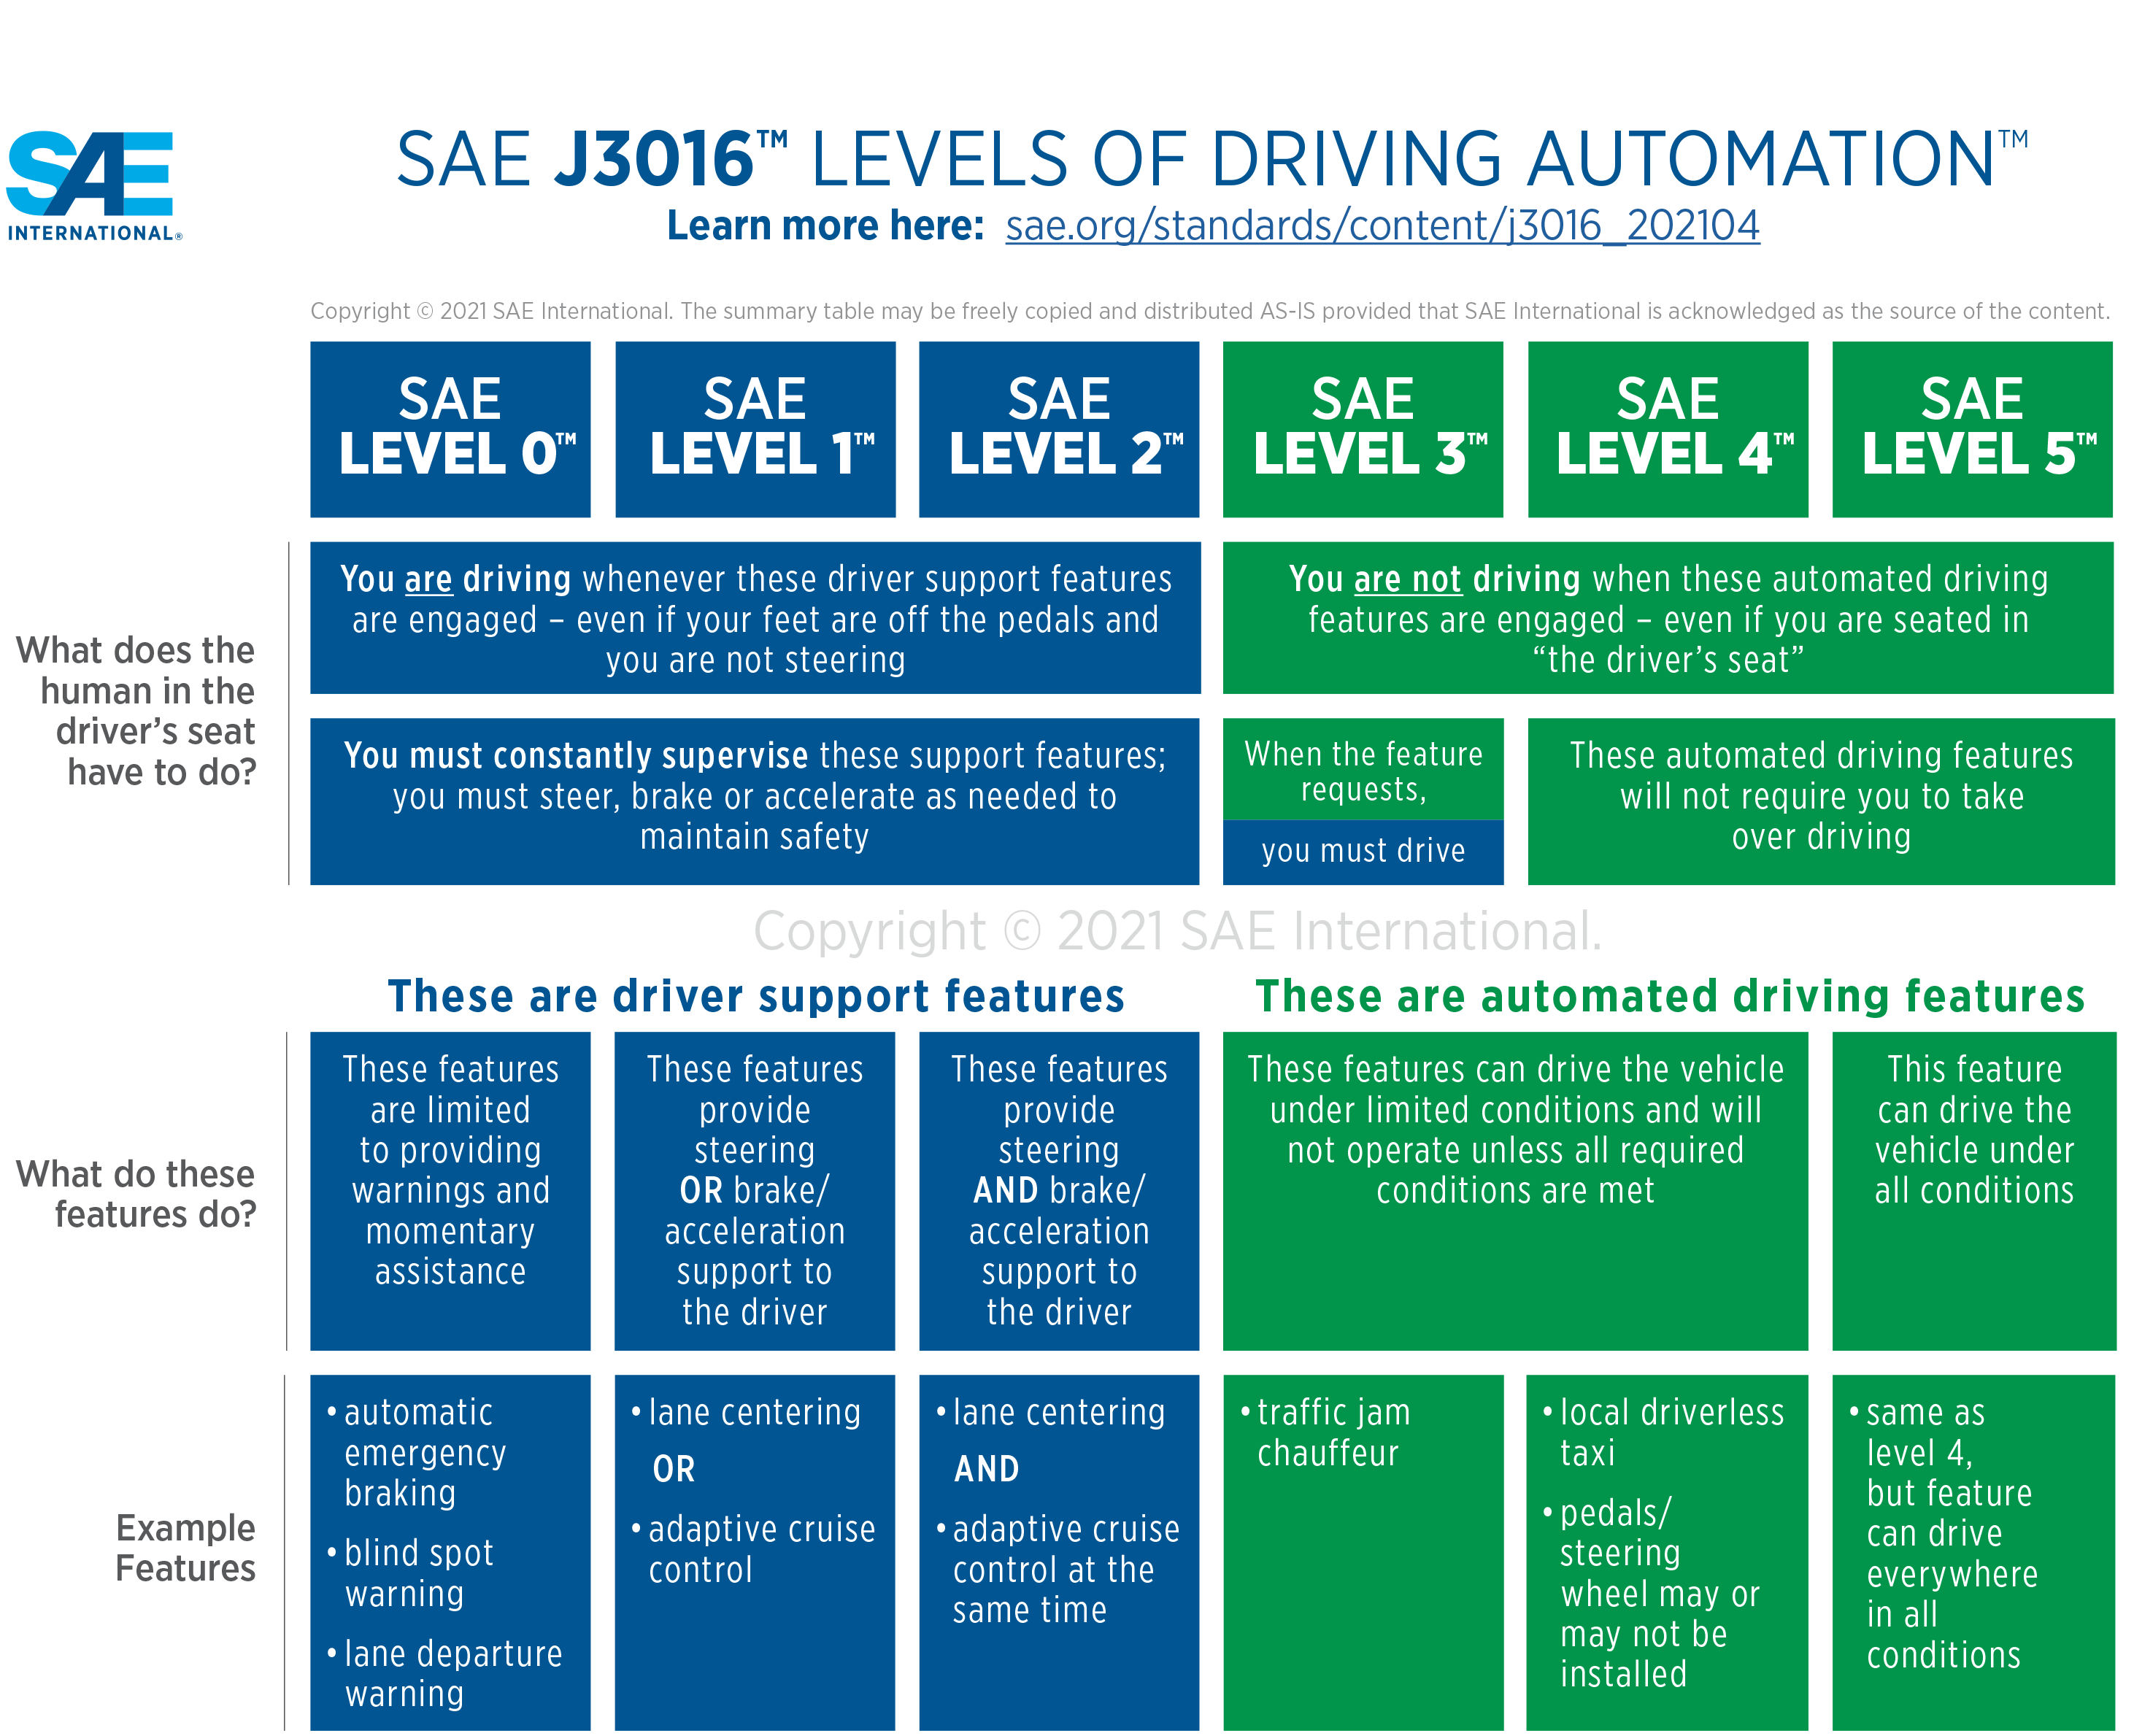
\includegraphics[width=\textwidth]{figures/SAE.png}
    \centering
    \caption{SAE Levels of Automation \cite{sae2021}}
    \label{fig:SAE}
\end{figure}

As of 2024, most advanced consumer vehicles operate at Level 2, with some manufacturers pushing towards Level 3 capabilities.
For example, BMW has recently become the first carmaker to receive approval for combining both Level 2 and Level 3 autonomous driving systems in a single vehicle.
The new BMW 7 Series now offers the BMW Highway Assistant (Level 2) and the BMW Personal Pilot L3 (Level 3), marking a significant step in automated driving technology \cite{bmw2024}.

At the forefront of \ac{AV} technology, companies like Waymo
are making significant strides towards Level 4 autonomy. Waymo has achieved
Level 4 autonomy in pilot areas, offering fully autonomous rides without safety
drivers in cities like San Francisco, Phoenix, and Austin \cite{evmagazine2024}.

 Achieving higher SAE levels of autonomy requires a sophisticated autonomous driving stack,
 which is composed of several vital modules that work together to perceive the environment,
 make decisions, and control the vehicle. The stack typically follows a modular software
 architecture that is shown in Figure \ref{fig:AVStack} integrates hardware and software components to enable safe and
 efficient vehicle operation.
 Modular software architecture is the predominant approach in \ac{AV} development, as it allows for separation of the
 modules and solve the issues separately. It startst with the perception module, which processes sensor data to understand
 the environment. Including mapping, localization, object detection, and tracking. The perception module feeds into the prediction
 where the vehicle anticipates the behavior of other road users and objects. The planning module then generates a trajectory for local
 and global scale. Finally, the control module executes the planned trajectory by sending commands to the vehicle's actuators. It is important
 to note that the perception module is the most critical part of the stack, as it provides the foundational data for all other modules. Any errors
 in perception can propagate through the entire system, leading to incorrect decisions and unsafe driving behavior.

\begin{figure}[h]
    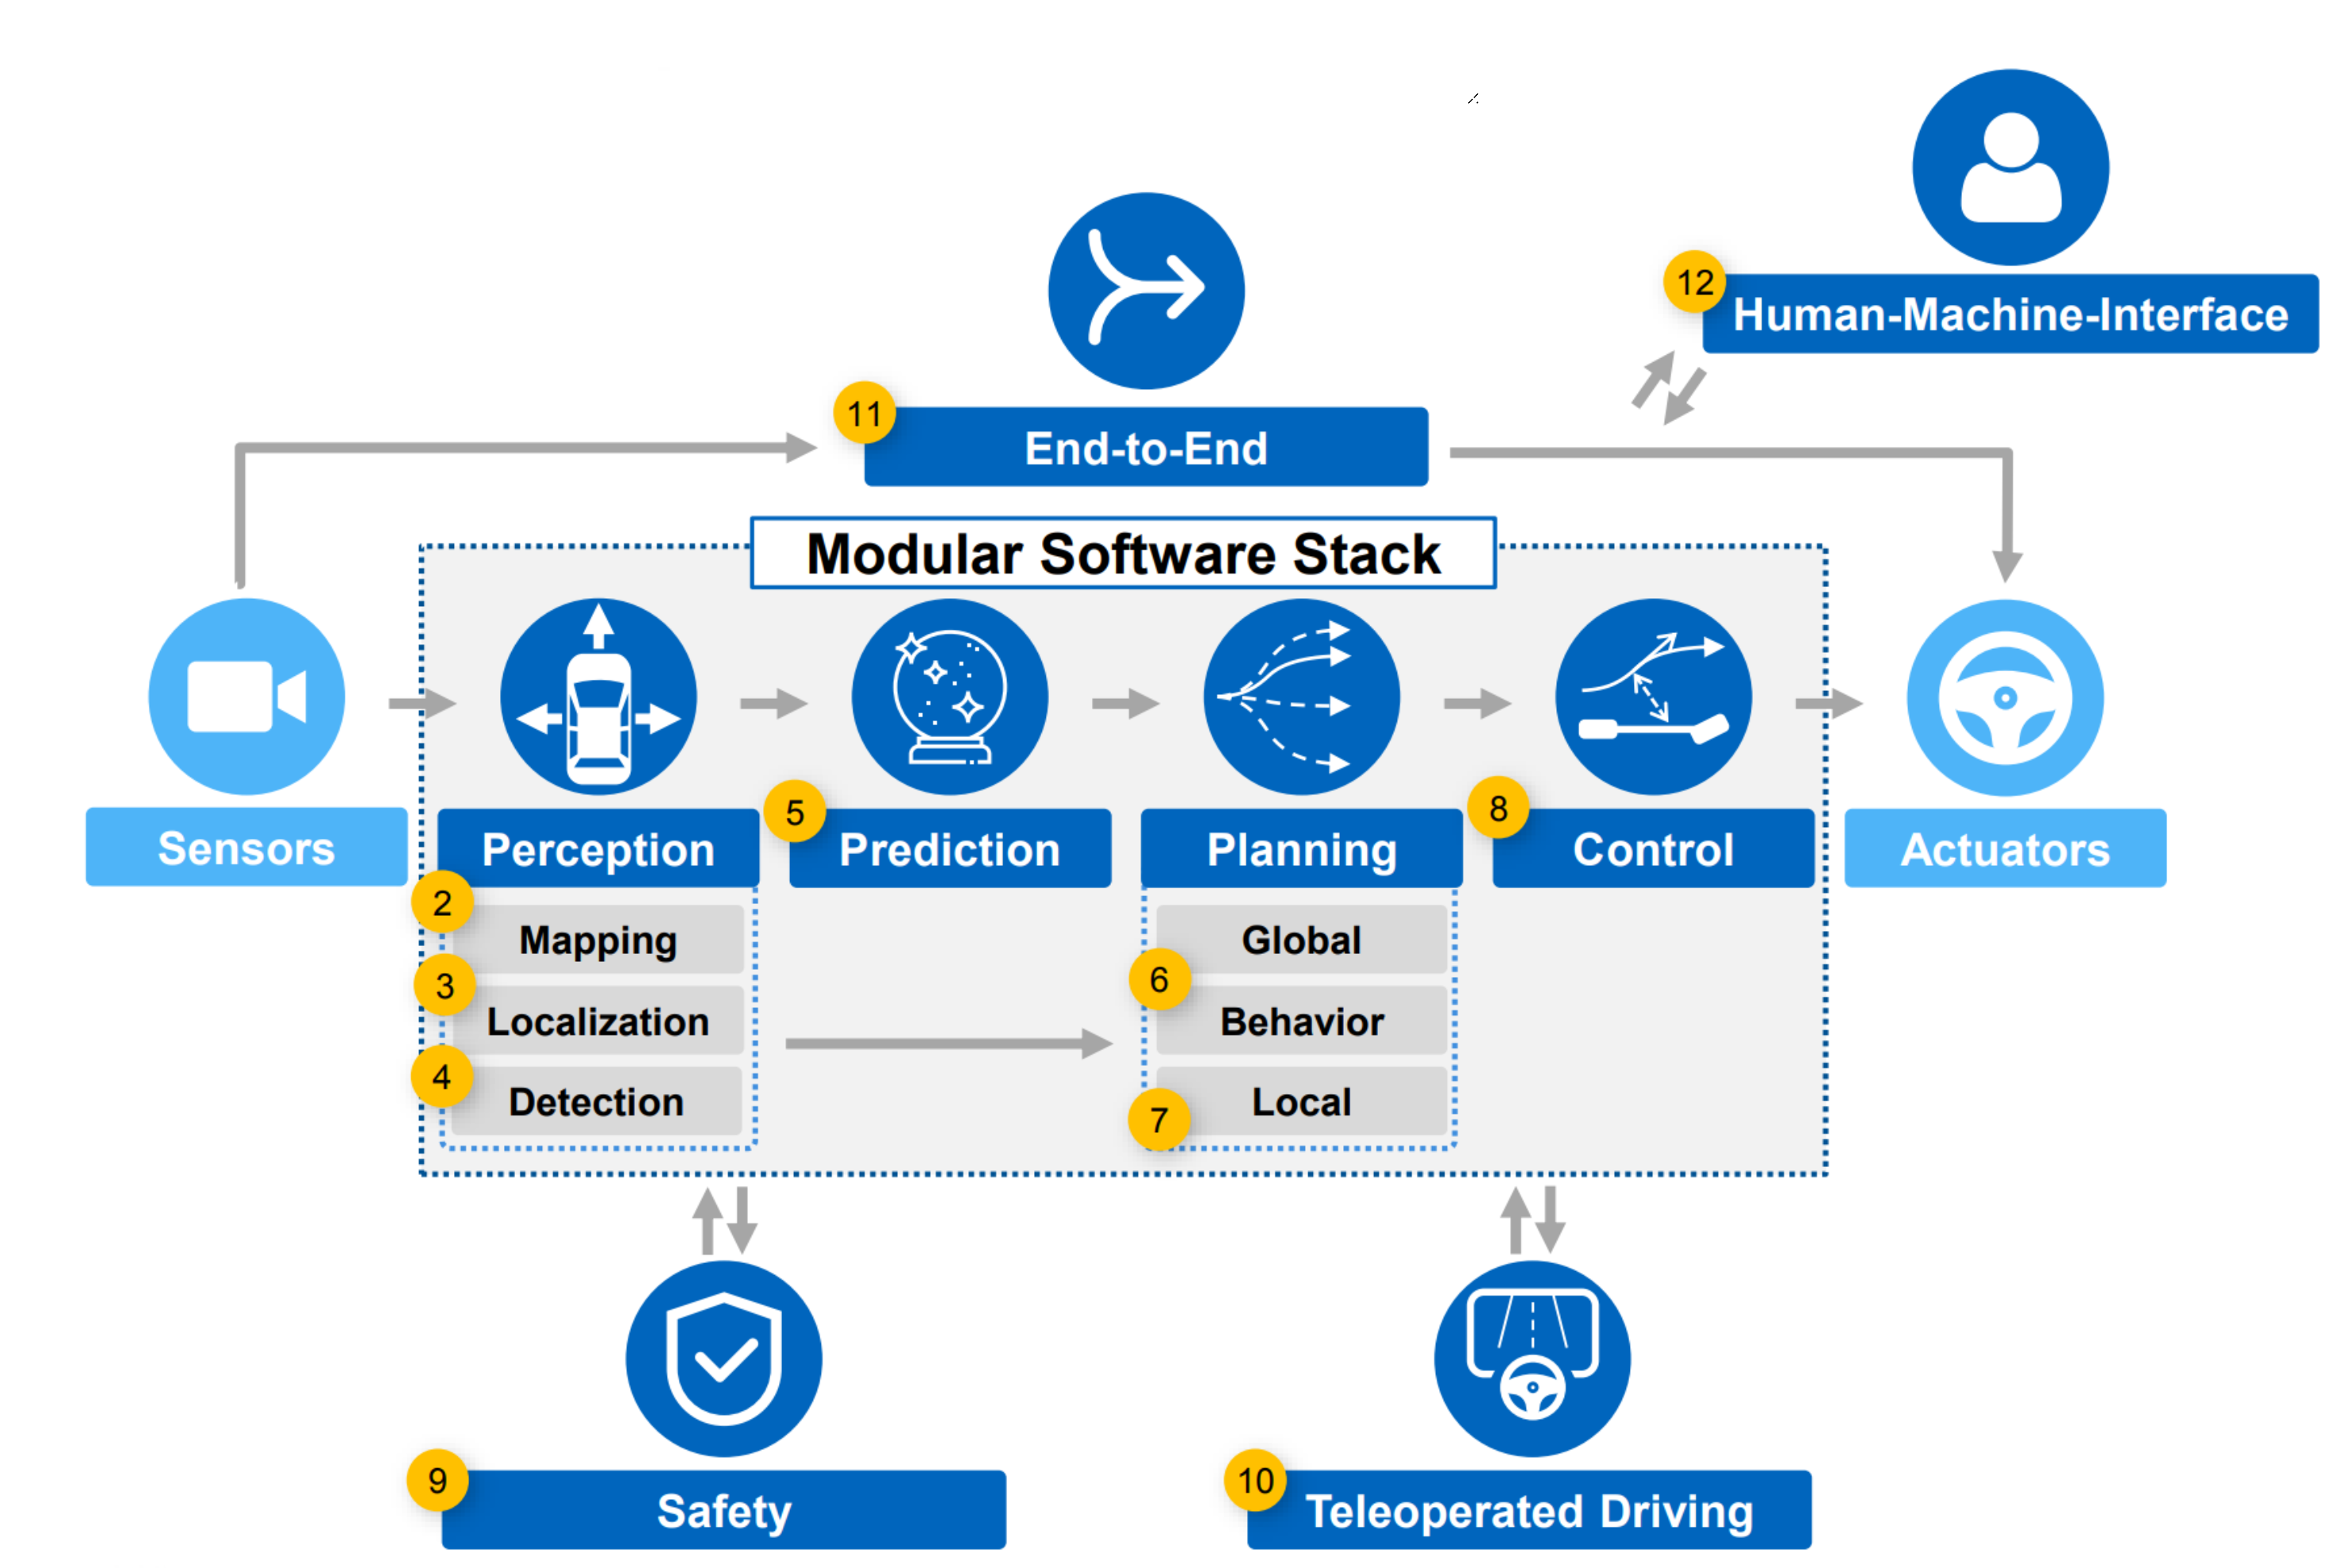
\includegraphics[scale=0.14]{figures/AVStack.png}
    \centering
    \caption{\ac{AV} Technology Stack
    from the lecture slides of "Software Engineering For Autonomous Driving" course, TUM, 2024 \cite{tum2024avstack}} %todo: add source from the lecture
    \label{fig:AVStack}
\end{figure}

While some research has explored end-to-end learning, where \ac{DL} models directly map sensor inputs
to control outputs without modular decomposition \cite{codevilla2019limitations}, this approach alone is often
insufficient for achieving higher levels of autonomy. End-to-end systems can struggle with interpretability
and adaptability across diverse driving scenarios \cite{e2e}. It is an active research area and some
of the mentioned issues can be solved with modular end-to-end learning \cite{nvidia2022diffstack} and also
it is expected to have a better performance on end-to-end methods with the improving hardware and datasets overtime \cite{e2e}.

For a system to reach higher SAE levels—particularly Level 4 or 5—all of
these modules must function reliably across various environments and conditions.
Each component plays a critical role in ensuring that the vehicle can navigate complex urban
environments safely and efficiently while responding to dynamic changes in real-time.
On the \acp{AV} with an automation level of 3 or lower, the driver must be ready to take over the control
when the system reaches its limits. This is called the "Handover" process.
But for the higher levels of automation, the vehicle must be able to handle the edge cases without an onboard human driver.
For that reason, we have teleoperation for the the cases where one or more module fails to deal the edge cases.
Teleoperation serves as a bridge between current autonomous driving capabilities and fully autonomous operation.
It allows vehicles to complete their missions even when their onboard systems encounter limitations.
For instance, if an \ac{AV} encounters a situation outside its \ac{ODD} \cite{iso34503},
such as unclear road markings or interactions with law enforcement, it can pull over safely and request human
intervention through teleoperation.
This technology is essential for ensuring that Level 4 and 5 \acp{AV} can operate reliably in real-world conditions
and is expected to play a key role in the widespread adoption of these \acp{AV}.


\subsection{Types of Data used in \acp{AV}} \label{subsection:sensors}
\acp{AV} rely on a diverse array of sensors and data sources to perceive their environment and gather the necessary
information for safe and efficient navigation. These sensors provide raw data that is
processed by the vehicle's perception system to understand
its surroundings, detect obstacles, and make real-time
decisions \cite{thrun2006stanley}.
In this thesis, we refer to this unprocessed data as
"Raw data" or "Raw sensory data." Additionally to the sensory data,
offline HD maps serve as a critical source of pre-processed environmental information,
complementing real-time sensor data with detailed static information about road layouts
and traffic elements \cite{bansal2018hdmaps,zhu2021hdmaps}.

\textbf{\ac{LiDAR}:}
    \ac{LiDAR} sensors use laser pulses to measure distances between the vehicle and surrounding objects.
    By emitting laser beams and measuring the time it takes for them to reflect back, \ac{LiDAR} creates
    a detailed 3D map of the environment. This technology is particularly useful for detecting objects'
    shapes, sizes, and positions with high accuracy, even in low-light conditions \cite{levinson2011towards}.
    \ac{LiDAR} is widely used in \ac{AV} systems due to its precision in mapping the surrounding area.

\textbf{Radar}:
    Radar sensors use radio waves to detect objects and measure their speed and distance from the vehicle.
    Unlike \ac{LiDAR}, radar is less affected by adverse weather conditions such as rain or fog, making it a
    reliable sensor for detecting moving objects like other vehicles or pedestrians \cite{patole2017automotive}.
    Radar is often used for functions like adaptive cruise control and collision avoidance.

    \textbf{Cameras}:
    Cameras capture visual data from the environment, providing rich information about road signs,
    lane markings, traffic lights, and other vehicles. \acp{AV} typically use multiple cameras positioned
    around the vehicle to achieve a 360-degree view \cite{geiger2012we}. Cameras are crucial for tasks requiring
    high-resolution visual data, such as object classification and scene understanding.

    \textbf{Ultrasonic Sensors}:
    Ultrasonic sensors are commonly used for short-range detection tasks like parking assistance or detecting nearby
    obstacles at low speeds. These sensors emit sound waves and measure their reflections to detect objects within
    a few meters of the vehicle \cite{zhang2018ultrasonic}.

    \textbf{Depth Cameras}:
    Depth cameras combine RGB imaging with depth sensing capabilities, providing both visual and spatial information about the environment \cite{aivero2024depth}.
    These sensors typically use dual cameras that enable stereo vision for depth perception, detecting position, distance, and speed of nearby objects \cite{aivero2024depth}.
    While \ac{LiDAR} remains crucial for \acp{AV}, depth cameras serve as an important complementary sensor, particularly effective at tracking multiple objects in close proximity \cite{argui2023mixed}.

    Compared to \ac{LiDAR}, depth cameras offer advantages such as lower cost and better performance in detecting small objects within their sensing range. Modern depth cameras like the FRAMOS D455e use active IR stereo technology with global shutter sensors, enabling accurate depth perception even with fast-moving objects \cite{framos2024d455e}. However, their effective range is typically limited to 0.6 to 6 meters, making them most suitable for near-field perception in \acp{AV}.

    \textbf{\ac{GPS}}:
    \ac{GPS} provides location data by triangulating signals from satellites. While GPS alone may not offer the precision
    required for autonomous driving, it is often combined with other localization methods such as \ac{SLAM}
    to improve accuracy \cite{thrun2005slam}.

    \textbf{\ac{IMU}}:
    The \ac{IMU} measures the vehicle's acceleration and angular velocity using accelerometers and gyroscopes.
    This data helps track the vehicle's movement and orientation in real time, contributing to accurate
    localization when combined with GPS data \cite{madgwick2011imu}.

    \textbf{Offline HD Maps:}
    Offline HD maps provide detailed information about road layouts, traffic signs, lane markings, and other static features of the driving environment. These maps enhance \ac{SA} by offering context beyond what onboard sensors can perceive in real time. HD maps are particularly useful for improving localization accuracy when combined with GPS and IMU data \cite{bansal2018hdmaps}. They also assist in path planning by providing precise information about road geometry, which is critical for autonomous navigation \cite{zhu2021hdmaps}.

We referenced a subset of TUM's EDGAR research vehicle's sensor setup as our basis.
EDGAR is equipped with 10 camera sensors, 4 \ac{LiDAR} sensors (long and short-range), 6 RADAR sensors as well as \ac{GPS}, \ac{IMU} and microphones \cite{tum2023edgar}.

\subsection{Perception Systems in \acp{AV}}
Perception systems are an essential component of \acp{AV}, responsible for interpreting the
vehicle's surroundings and enabling safe navigation. They are the basis of the modular software stack from \ref{fig:AVStack}.
These systems process data from sensors such as \ac{LiDAR},
radar, and cameras to detect and classify objects, track their movements, and localize the vehicle within
its environment \cite{liu2018perception}. The perception system builds a comprehensive model of the environment,
which is then used by other modules—such as prediction, planning, and control—to make driving decisions.

This thesis will refer to "Perception Data" as the processed output from the vehicle's perception system. This includes information about detected objects (e.g., vehicles, pedestrians), their classifications, positions, and trajectories. The perception system also generates high-level semantic information such as lane markings, traffic signs, and road boundaries. This data enables \acp{AV} to understand their environment and make informed decisions.

We utilize Autoware, an open-source software stack designed for autonomous driving systems for all perception-related tasks in this project. Autoware provides a comprehensive set of tools for processing sensor data and generating perception outputs \cite{kato2018autoware}. It includes object detection, classification, tracking, and localization modules using sensors such as \ac{LiDAR}, radar, and cameras. By leveraging Autoware's robust perception capabilities, we ensure that our system can handle complex environments while maintaining flexibility for future improvements.

Autoware also supports sensor fusion techniques that combine data from multiple sensors to improve accuracy and reliability. This is especially important when dealing with noisy or incomplete sensor data. For instance, Autoware's fusion algorithms can combine \ac{LiDAR} point clouds with radar measurements to enhance object detection
performance in adverse weather conditions where cameras may struggle.
\section{Teleoperation Concepts} \label{section:teleoperation}

Teleoperation is an essential fallback solution for \acp{AV},
enabling a human operator to remotely assist or take control of a vehicle when
its automated systems encounter situations beyond their \ac{ODD}
or face disengagements. These scenarios often arise due to complex or unforeseen edge cases,
such as sensor malfunctions, unanticipated obstacles, or ambiguous road conditions.
The system ensures that the \ac{AV} can resume its mission safely and efficiently \cite{Brecht}.

Several teleoperation concepts have been developed to address different aspects of remote vehicle control, each with its own strengths and limitations. These concepts can be broadly categorized into Remote Driving and Remote Assistance with subcategories. Each approach targets specific challenges in teleoperation, such as latency, \ac{SA}, and operator workload.

\subsection{Remote Driving}
Remote Driving is one of the earliest teleoperation concepts,
where a human operator takes full control of the vehicle's
dynamic driving tasks, including steering, acceleration,
and braking. This concept has been explored for more than two decades.
Early research by Sworder et al. \cite{sworder1999performance} (1999) demonstrated the feasibility
of teleoperating vehicles using direct control methods, where
operators manually control vehicles based on live video feeds and
sensor data transmitted from the vehicle to a remote station.
This method, known as Direct Control, has been widely studied
and implemented in various industries since then \cite{Gnatzig,chucholowski2014teleoperated,Tang}.

Despite its long history, Direct Control remains relevant
today due to its simplicity and directness. In this approach,
the operator receives real-time video and sensor data from the
vehicle and sends back control commands such as steering angles
or velocity adjustments. However, this method is highly sensitive
to network conditions—particularly latency and bandwidth
limitations—which can lead to reduced \ac{SA} for
the operator and delayed reactions to dynamic situations \cite{Gnatzig}.
Latency is a critical factor in teleoperation; studies have shown
that latencies greater than 10 milliseconds can result in degraded
performance in high-speed or complex environments \cite{chucholowski2014teleoperated}.
Under fluctuating network conditions—such as handovers
between cellular towers or signal degradation due to obstacles—latency
can increase unpredictably, leading to delayed responses that
compromise safety \cite{neumeier2023feasibility}.

In recent years, several companies have implemented Direct Control
in real-world applications despite these challenges. For example,
Fernride, a Munich-based company, has successfully deployed
teleoperation technology for logistics operations. Fernride's
platform allows remote operators to control semi-autonomous
trucks in logistics yards using Direct Control methods.
In their pilot project with DB Schenker and KAMAG,
teleoperators remotely controlled trucks for yard shunting
tasks—moving trailers around loading docks—demonstrating that
teleoperation can be safely integrated into existing logistics
processes \cite{fernride2023}. The success of this project
highlights the potential of Direct Control in controlled
environments like logistics yards where network conditions are stable.

However, while Direct Control has proven effective in specific use cases
such as logistics yards or industrial environments with
controlled network conditions, it faces significant challenges when
applied to more complex or dynamic environments like urban roads.
The sensitivity of Direct Control to network latency makes it less
suitable for scenarios where real-time decision-making is critical for
safety. To mitigate these challenges, modern teleoperation systems
often incorporate additional safety measures or alternative methods
that reduce reliance on real-time control inputs.

One such alternative is Shared Control, where the vehicle retains
some level of autonomy while the operator provides the control inputs as in the Direct Control.
In this approach, if an operator's input does not meet
certain safety criteria—such as proximity to other vehicles—the
vehicle's onboard systems can override those commands to prevent
collisions \cite{kay2024sharedcontrol}. This approach reduces
cognitive load on the operator while ensuring that safety-critical
decisions are still handled by the vehicle's autonomous systems.

\subsection{Remote Assistance}
Remote Assistance focuses on providing high-level guidance or support
to specific functions of the AV without taking full control of the DDT.
This method is often used in scenarios where the AV encounters an
edge case that prevents it from continuing its mission autonomously
but does not require complete human intervention \cite{Brecht}.

In Waypoint Guidance, for example, operators provide waypoints or general
directions for the vehicle to follow while leaving detailed path planning
and execution to the AV's onboard systems \cite{corridor}. This reduces
operator workload but may lead to stop-and-go behavior if communication
between the operator and vehicle is not seamless.

Another promising approach is Collaborative Planning, where operators
work with the AV's planning system by selecting from a set of pre-generated
path suggestions based on sensor data. This method allows operators to focus
on decision-making rather than low-level control tasks \cite{hosseini2024collaborative}.
Collaborative planning improves efficiency but requires robust sensor fusion and reliable
perception data from the AV.
\subsection{Perception Modification}

Perception Modification is one of the most promising teleoperation
concepts within Remote Assistance category. Designed to address situations where an \ac{AV}
encounters perception errors that prevent it
from continuing its mission. These errors may arise from false
positives or misclassifications in the vehicle's perception system,
such as detecting an object that is not truly obstructing the path or
misinterpreting environmental features like lane markings or road signs.
In such cases, Perception Modification allows a remote operator to
intervene by modifying some elements of perception to correct \ac{AV}'s interpretation,
enabling it to resume its journey \cite{Feiler2021ThePM}.

In this concept, the operator has access to both raw sensor data
(e.g., \ac{LiDAR} point clouds or camera images) and processed perception
data (e.g., object classifications or environmental models).
By reviewing this data, operators can identify discrepancies
between what the vehicle perceives and what is present in its
surroundings. For example, if a false-positive detection is blocking
the vehicle's path—such as a plastic bag being detected as a solid
obstacle—the operator can modify or correct these perceptions by
marking the area as drivable. This correction enables the AV to
continue its mission without requiring complete manual control \cite{Feiler2021ThePM}.

The Perception Modification concept is beneficial because
it reduces the cognitive load on the operator compared to direct control methods.
Instead of managing all aspects of driving, operators focus solely on correcting
specific perception errors. This approach allows for more efficient human
intervention while minimizing the risk of operator fatigue or error due to
high mental workload \cite{Brecht}. Additionally, Perception Modification can
be extended beyond object detection corrections; operators could also modify other
aspects of the environmental model, such as lane boundaries or drivable space predictions.

As Feiler and Diermeyer \cite{Feiler2021ThePM} define it, the implementation of
Perception Modification involves integrating a  \ac{HMI} that provides operators with real-time access to both raw sensor data and processed perception data. The HMI allows operators to
mark areas as drivable or ignore specific detections deemed irrelevant or incorrect. The vehicle's planning module receives this modified perception data and generates a new trajectory based on these corrections.

In their comparative study of teleoperation concepts, Brecht et al. \cite{Brecht} found
that Perception Modification imposes less cognitive load on operators than
Direct Control while still enabling efficient resolution of disengagements.
The study also highlighted that Perception Modification is highly effective in
situations where false-positive detections or indeterminate objects hinder an AV's progress.
However, it may not be suitable for all disengagement scenarios—particularly those
involving complex trajectory planning failures or situations requiring immediate manual intervention.

\section{Environmental Data Visualization for \acp{AV}}
Environmental data visualization plays a fundamental role in \ac{AV} systems,
particularly in teleoperation scenarios where human operators must understand and interpret
complex sensor data to make critical decisions.
Visualizing environmental data is crucial for two reasons: First, it enables operators to
maintain high \ac{SA} during
teleoperation tasks \cite{Gnatzig}. Second, it allows for effective monitoring and verification
of the vehicle's perception system, essential for identifying and correcting potential errors
in the automated driving system \cite{Feiler2021ThePM}.

\subsection{Challenges in Visualizing Multi-Sensor Data}\label{subsection:challengesmultisensor}
One of the primary challenges in environmental data visualization is integrating data from multiple
sensors into a cohesive representation of the environment. Modern \acp{AV} generate
massive amounts of data - up to 3-6 TB of raw data per hour of operation from their sensor suite \cite{kazhamiaka2021challenges}
. A single 4K camera operating at 30 frames per second can produce
approximately 5.4 TB per hour, while a typical AV may have 6-12 cameras along with other sensors \cite{visualcapitalist2024}
. This creates a significant challenge in data processing, transmission,
and visualization. Each sensor type has strengths and limitations, as defined in Section \ref{subsection:sensors}.

The sensor fusion process combines these different data streams into a single, a unified environmental
model that is used by nearly all parts of the autonomous driving stack like perception system \cite{feng2020deep}
, localization system \cite{feng2020deep, el-sheimy2020sensorfusion}. It can also be used for the human operator interface.
However, visualizing this fused data presents several challenges:

\textbf{Real-Time Processing:} Processing and visualizing sensor data in real time requires significant computational resources. Delays in processing can lead to outdated information being presented to the operator, reducing \ac{SA} \cite{Gnatzig}.

\textbf{Accuracy vs. Latency:} High-fidelity visualizations may improve accuracy but come at the cost of increased latency. A balance between these two factors must be kept for effective teleoperation \cite{chucholowski2014teleoperated}.

Data overload is particularly sensitive in teleoperation scenarios, where operators must quickly understand and respond to complex environmental data while maintaining real-time awareness of the vehicle's situation. This requires careful consideration of which data to present and how to present it effectively without overwhelming the operator's cognitive capabilities.

\subsection{Human Factors in Perception Data Visualization}\label{subsection:humanfactors}
We consider two critical elements in teleoperation in the aspect of human factors: \ac{SA} and mental workload. These factors significantly influence an operator's ability to effectively control and monitor remote vehicles.

\textbf{Situational Awareness:} In teleoperation scenarios, achieving and maintaining \ac{SA} presents unique challenges due to the physical separation between the operator and the vehicle. Gnatzig et al. \cite{Gnatzig} shows that operators must rely entirely on sensor data and interface representations to understand the remote environment, making the quality and presentation of this information critical for effective operation.  As Endsley \cite{endsley1995toward} states, "Even the
best-trained decision makers will make the wrong decisions if they have inaccurate or incomplete SA.".

\textbf{Mental Overload:} Presenting all sensor data simultaneously can overwhelm operators with too much information.
Operators must process and integrate information from multiple sources while maintaining awareness of critical events, which can lead to increased mental workload \cite{wickens2008multiple}.

\section{Existing Approaches to Visualizing Sensor Data}
The visualization of sensor data and perception outputs is crucial for developing and monitoring \acp{AV}. Various approaches have been developed by both industry and academia to address the challenges of presenting complex environmental data effectively. This section examines existing visualization solutions, starting with industry standards and progressing to more specialized approaches.
\subsection{Industry Standards}
Major \ac{AV} companies have developed sophisticated operator interfaces to support remote monitoring and intervention when autonomous systems face complex or ambiguous scenarios. These interfaces are designed to provide comprehensive environmental awareness by integrating real-time sensor data, perception outputs,
and vehicle behavior into an accessible format. Below, we highlight examples of operator-focused visualization systems developed by leading companies.

Waymo's Fleet Response Interface \cite{waymo2024fleetresponse}, shown in figure \ref{fig:Waymo} is a prime example of a teleoperation tool designed for remote intervention. This interface provides a detailed 3D visualization of the vehicle’s surroundings, integrating \ac{LiDAR} point clouds, camera feeds, and object detection data in real-time. Remote operators can monitor the vehicle’s perception system and provide guidance when necessary. For instance, operators can review live video feeds and rewind past footage to better understand complex situations such as construction zones or ambiguous road markings. The system allows operators to suggest lane changes or route adjustments while ensuring the Waymo Driver remains in complete vehicle control.

\begin{figure}
    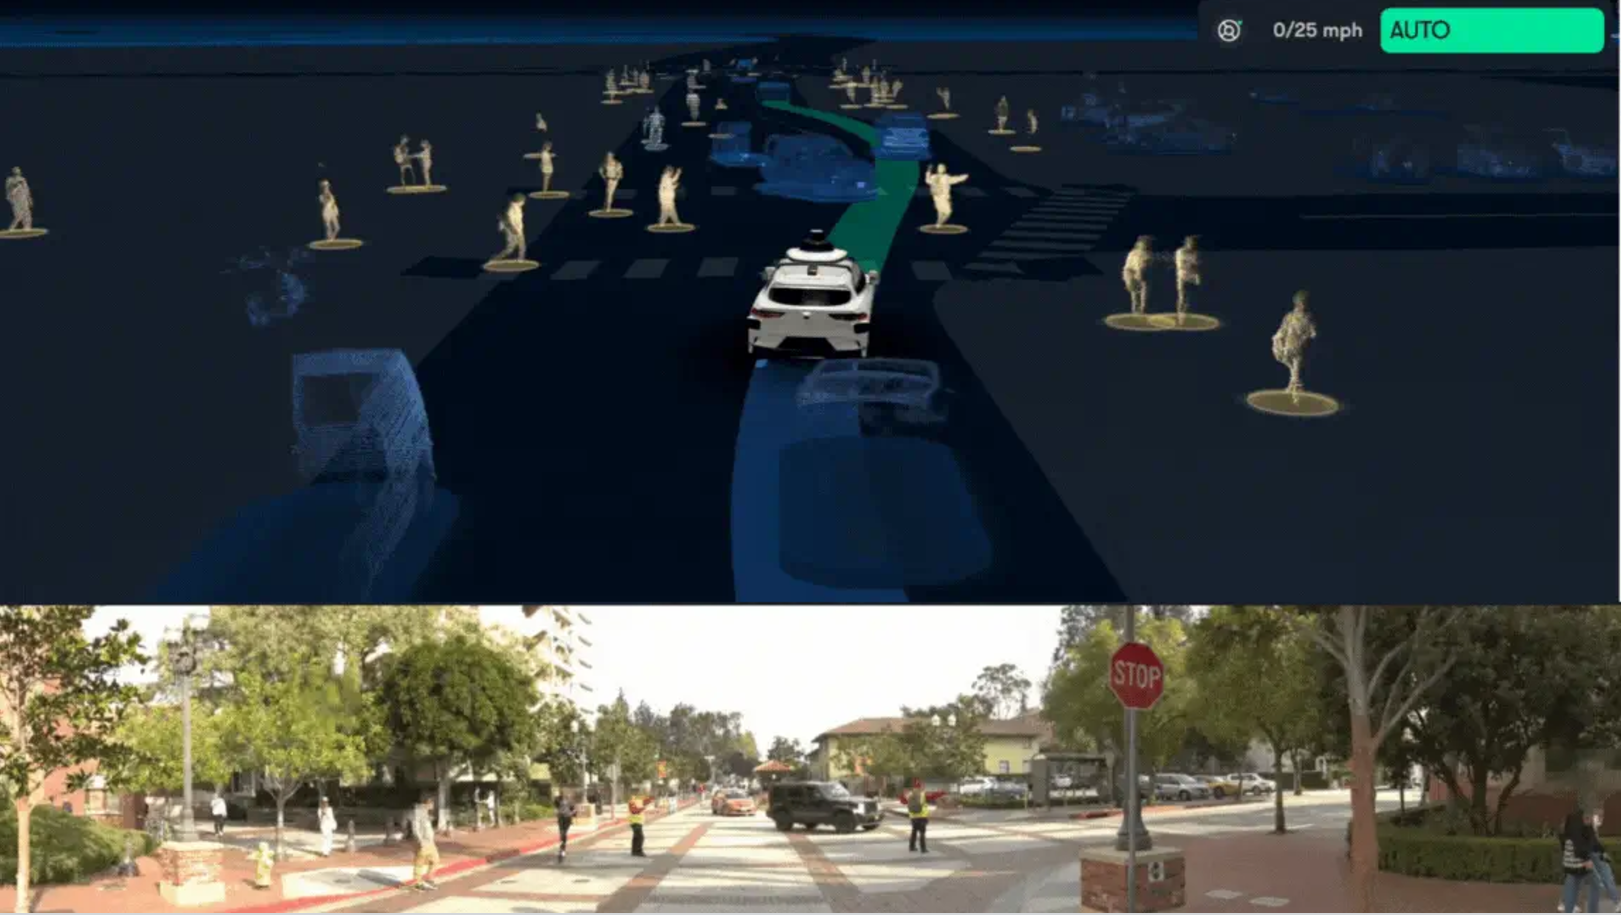
\includegraphics[width=0.8\textwidth]{figures/waymo.png}
    \centering
    \caption{Waymo's Fleet Response Interface \cite{waymo2024fleetresponse}}
    \label{fig:Waymo}
\end{figure}

Zoox's TeleGuidance System \cite{zoox2024teleguidance} is another example of an operator interface designed for remote assistance. Like Waymo’s system, Zoox provides a separate view of the camera feed and a 3D environment model of the vehicle’s perception. This system allows the operator to do both waypoint guidance
 \cite{corridor} and also a subset of perception modification \cite{Feiler2021ThePM} by object recategorization.

\begin{figure}
    \centering
    \begin{subfigure}[b]{0.48\textwidth}
        \centering
        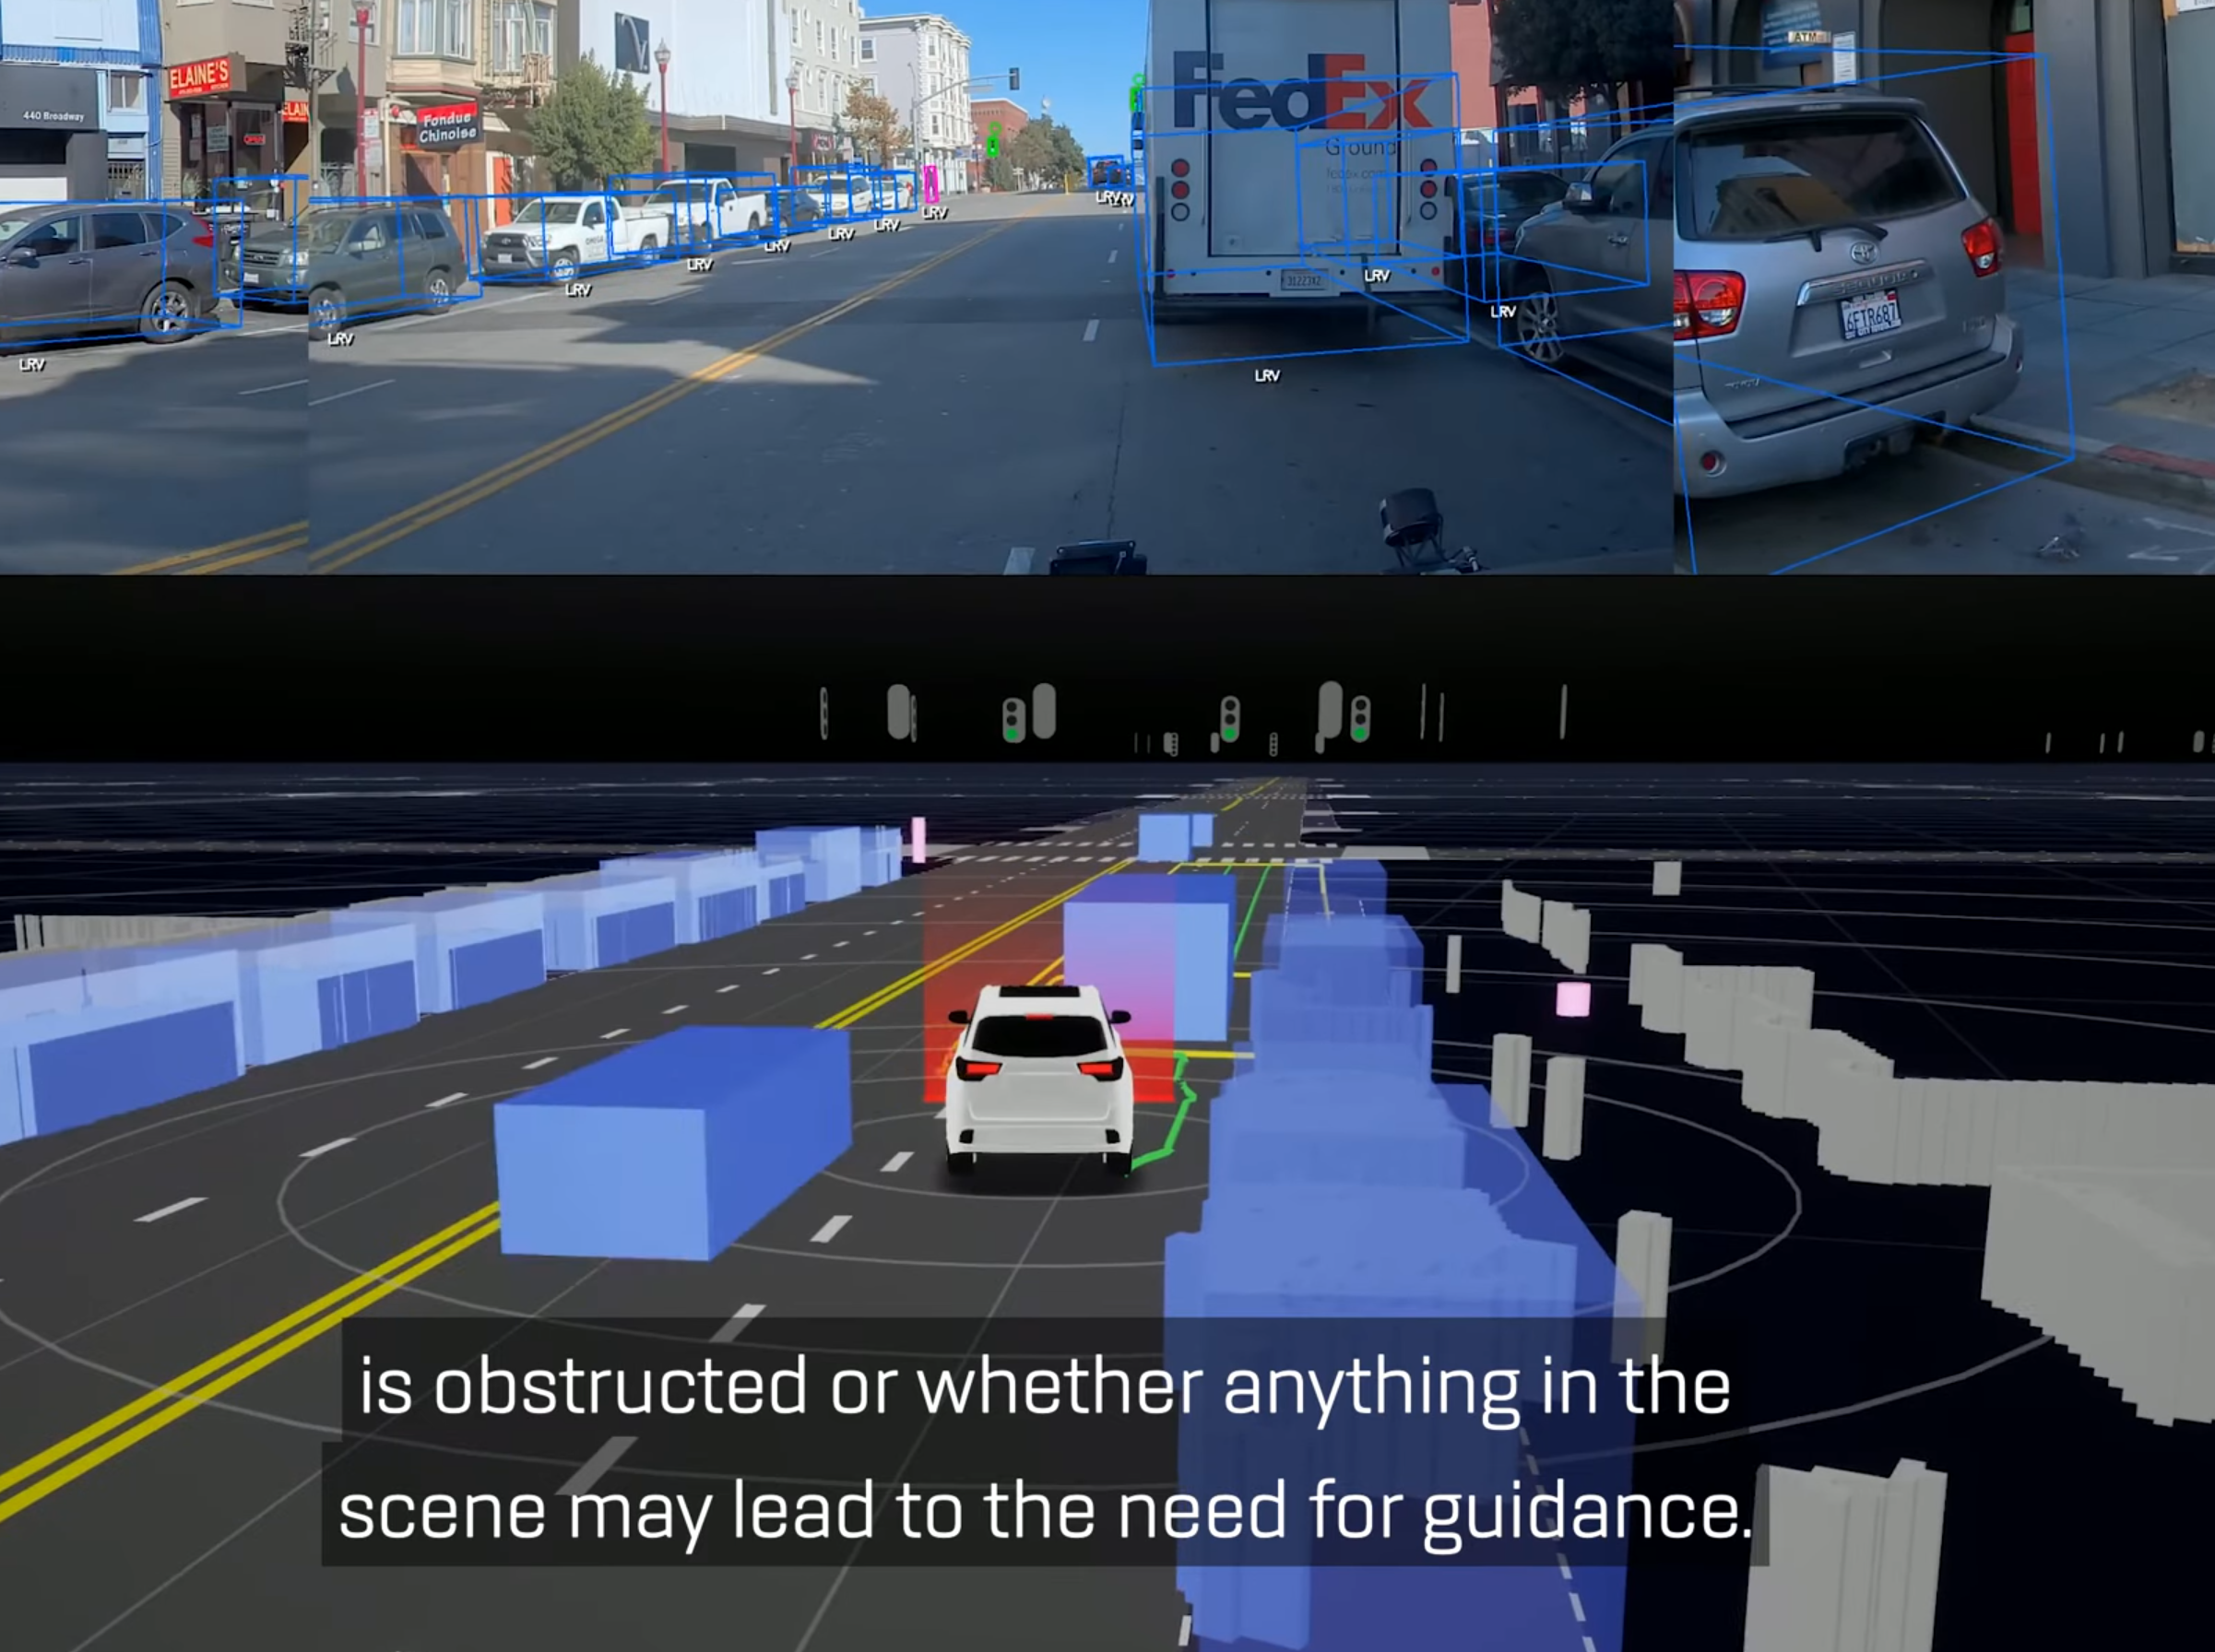
\includegraphics[width=1\textwidth]{figures/zoox.png}
        \caption{Zoox's TeleGuidance System}
        \label{fig:Zoox}
    \end{subfigure}
    \hfill
    \begin{subfigure}[b]{0.48\textwidth}
        \centering
        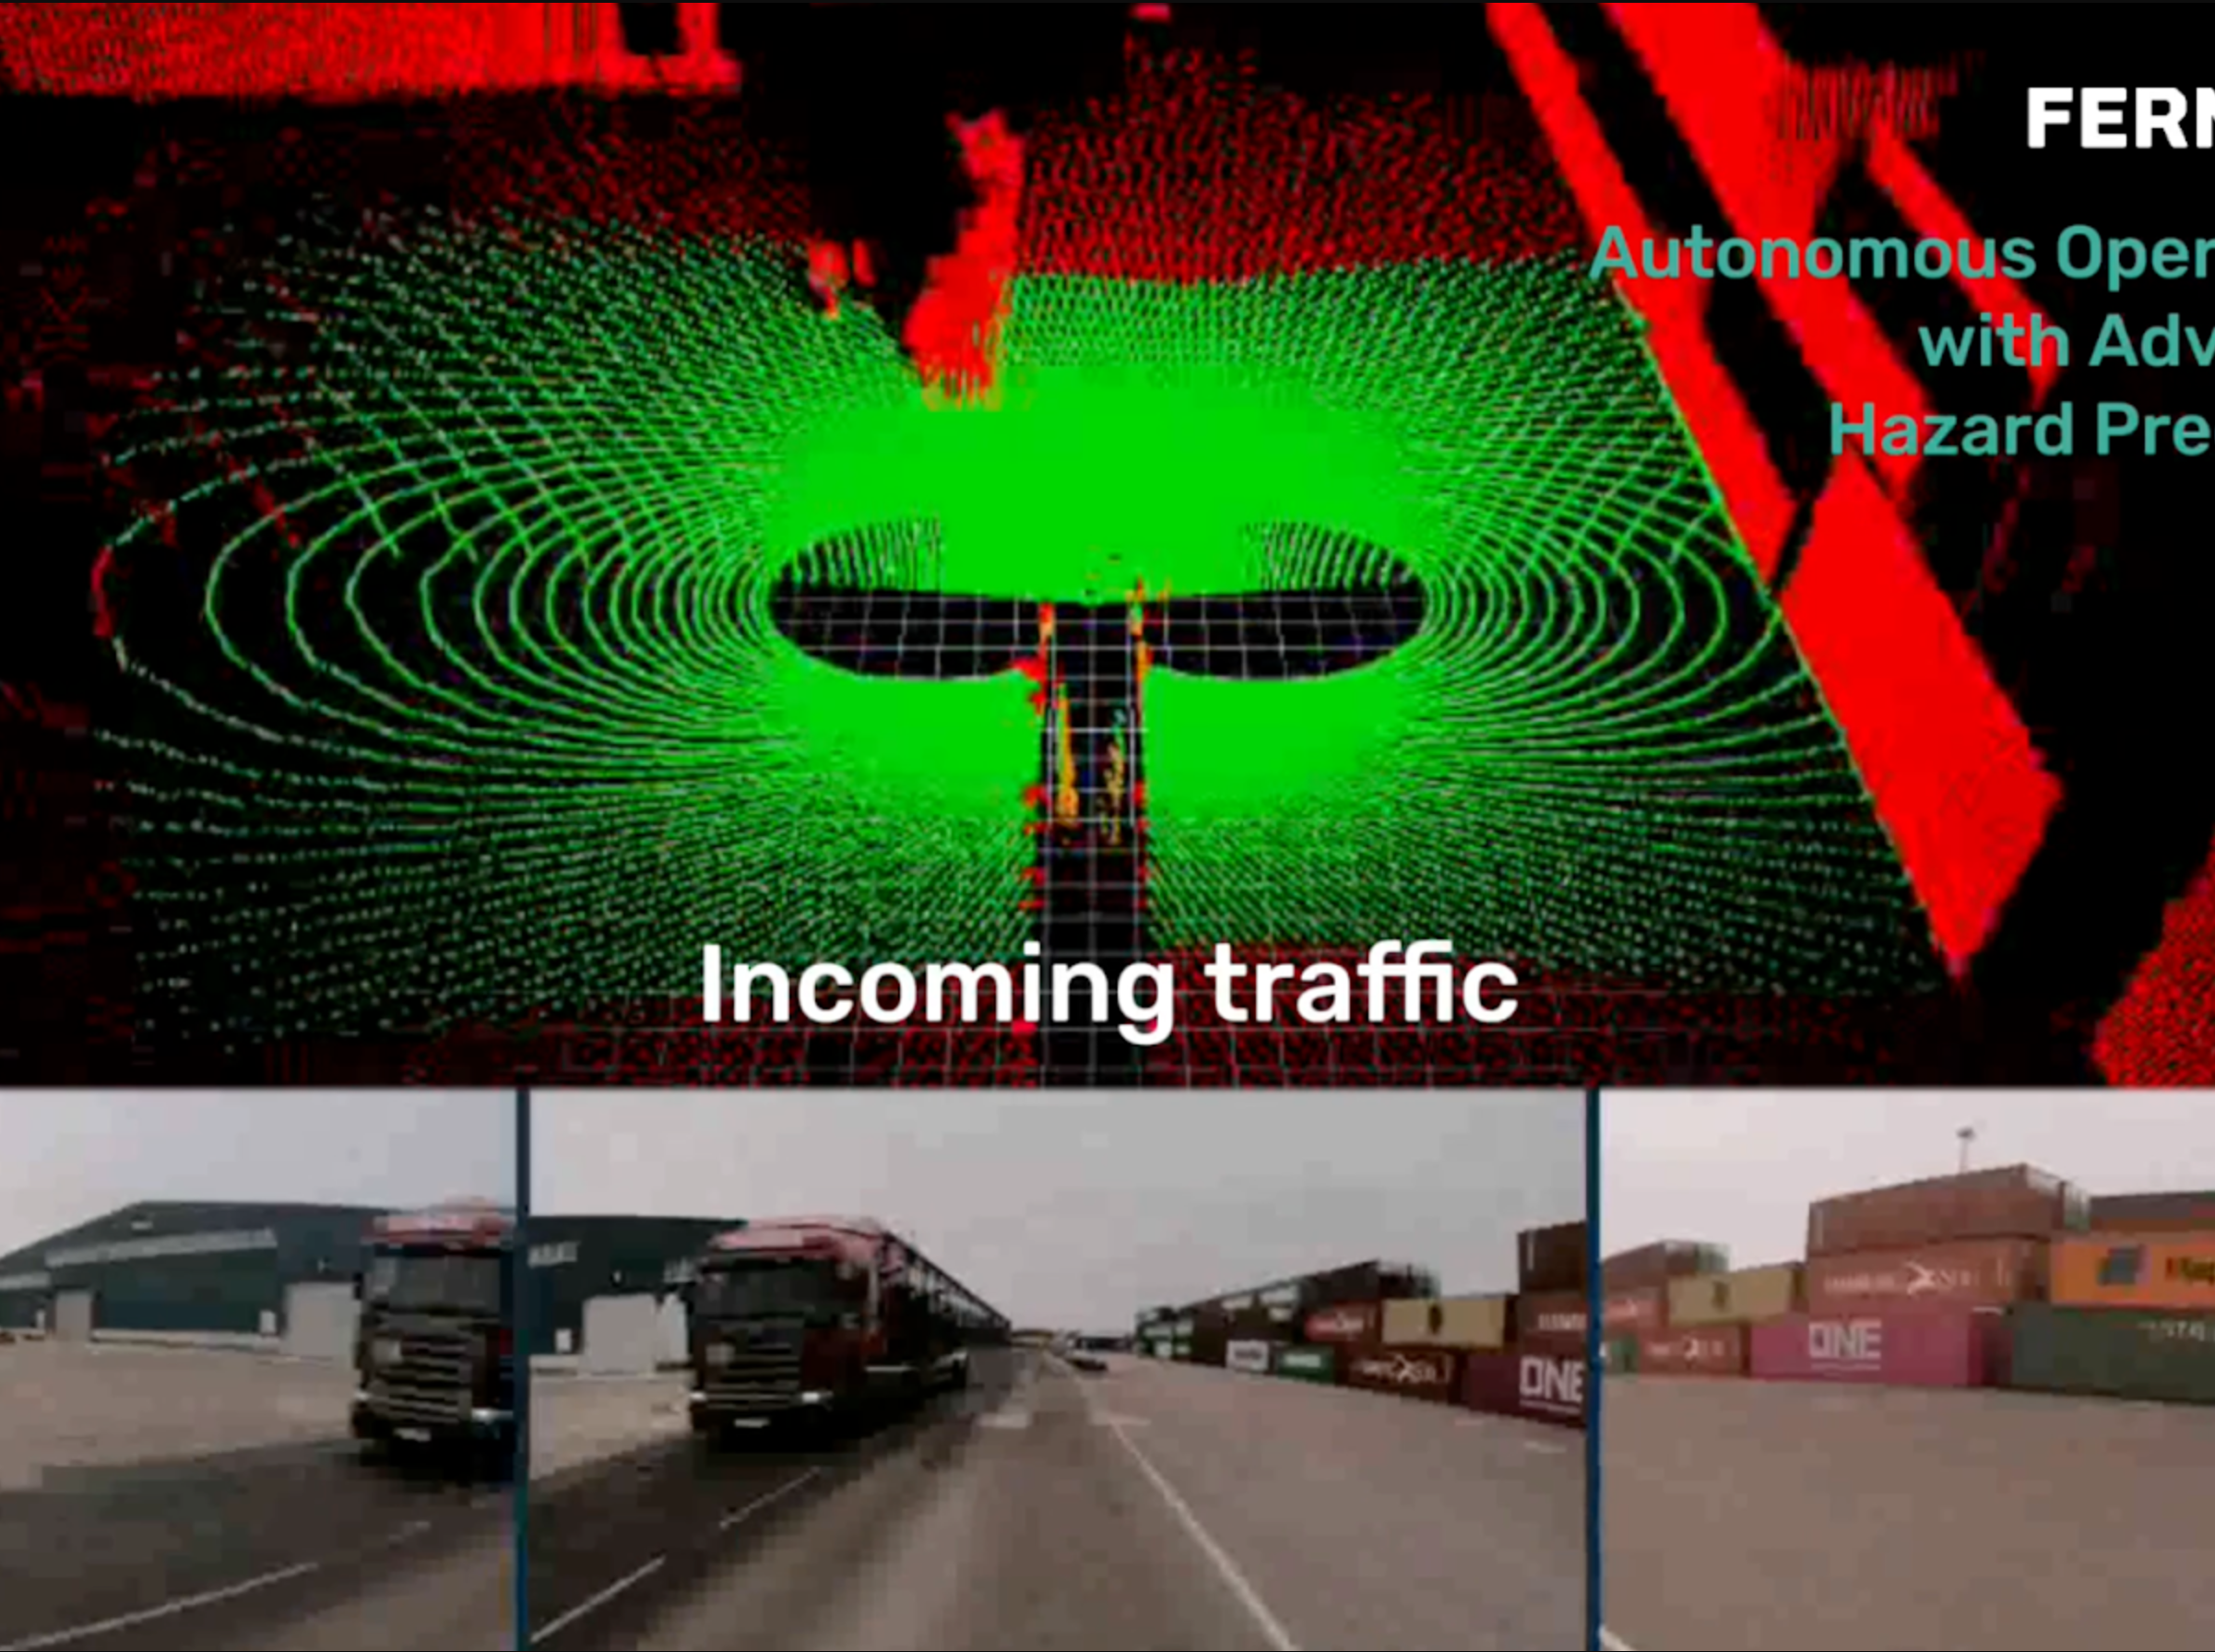
\includegraphics[width=1\textwidth]{figures/fernride.png}
        \caption{Fernride's Teleoperation Interface}
        \label{fig:Fernride}
    \end{subfigure}
    \caption{Comparison of Interfaces for Remote Assistance(a) and Direct Control(b)}
    \label{fig:TeleoperationComparison}
\end{figure}

As shown in \ref{fig:Zoox}, They also provide some perception information mixed in with the video feed.

Fernrides' strategy is different from the other two. They provide a direct
control interface for their teleoperation system. The operator can control the vehicle directly with a joystick and monitor the vehicle's surroundings with a 360-degree camera feed. This approach suits controlled environments like logistics yards, where real-time control is essential for efficient operations \cite{fernride2023}. Since their level of autonomy is lower than that of other examples, the need for perception visualization is also lower. Thus, they focus more on the raw sensory data representations.

\subsection{ToD Visual 2.0}\label{subsection:todvisual}
The software stack on which we are building our interfaces is based on ToD Visual 2.0, a teleoperation visualization software developed by the TUM Institute of Automotive Technology. This software is an improved version of ToD Visual \cite{Schimpe}, initially developed for the TUM EDGAR research vehicle. The new version introduces a modular structure, allowing for the easy integration of various visualization approaches and customization to meet specific use cases.ToD Visual 2.0 has already been showcased in public as part of the TUM Wiesn Shuttle event, where it was used to display sensory and perception data during the autonomous shuttle's operation in the challenging traffic conditions surrounding Munich's Oktoberfest \cite{adac2024wiesn, tum2024wiesn}. This real-world demonstration highlighted the software's capabilities in rendering complex sensor data and providing meaningful insights into vehicle behavior under extreme conditions. Although ToD Visual 2.0 is not yet open-sourced, plans are underway to make it publicly available. This will enable broader adoption and collaboration within the research and development community. The software stack provides robust capabilities for rendering sensory information, such as point clouds from \ac{LiDAR}, camera images, and radar data. Additionally, it supports visualization of perception outputs, including:
\begin{itemize}
    \item Bounding boxes with color-coded classifications for object detection,
    \item Trajectory information for planned vehicle paths,
    \item Lane information derived from offline HD maps.
\end{itemize}

\begin{figure}
    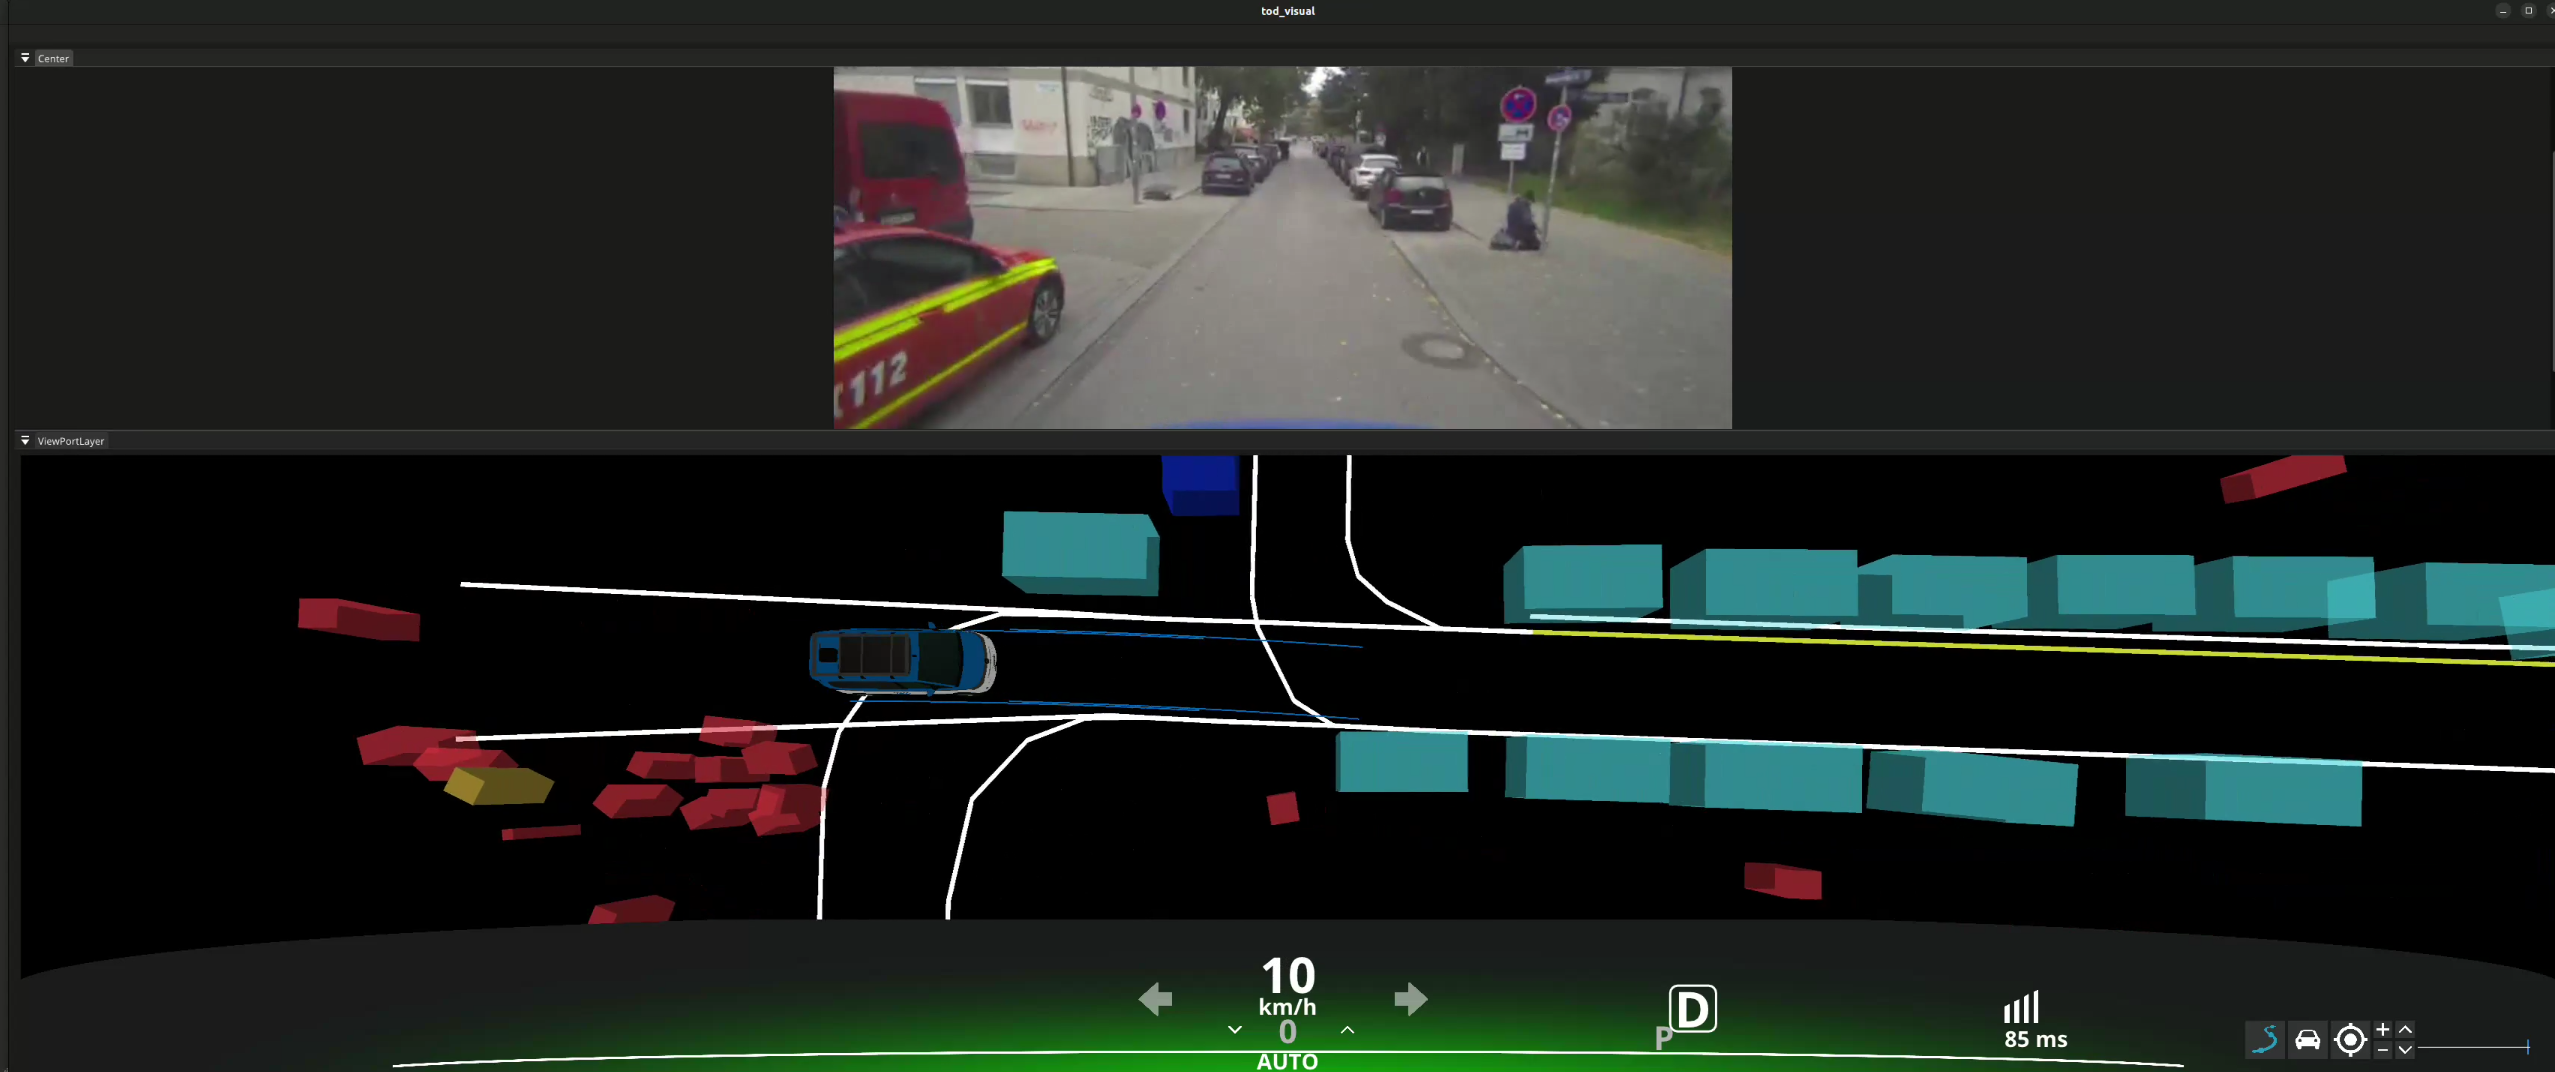
\includegraphics[width=0.8\textwidth]{figures/tod_visual.png}
    \centering
    \caption{ToD Visual 2.0 Interface from Wiesn' Shuttle Event}
    \label{fig:ToDVisual}
\end{figure}

The interface before our contribution within this paper can be seen in Figure \ref{fig:ToDVisual}.

For this thesis, we have taken ToD Visual 2.0 as a foundation and enhanced several components to align with our specific use case. These improvements include refining existing features and adding new functionalities tailored to support our Separate View and Integrated View approaches.


\subsection{Separate View}\label{section:separateview}
In this section, we define the Separate View visualization approach, which involves presenting 2D and 3D data in distinct windows or displays for the operator. This method allows operators to view the 2D data (e.g., camera images) alongside processed perception outputs and raw 3D data (e.g., object detections, \ac{LiDAR} point clouds) in separate, clearly delineated spaces. By separating these views, operators can compare the raw data against the system's perception outputs to identify potential discrepancies, such as misclassifications or false positives.

The Separate View approach is particularly advantageous for teleoperation scenarios where \ac{SA} and perception verification are critical. Operators can use the 2D view to observe raw camera feeds for a direct visual understanding of the environment, while the 3D view provides a synthesized representation of the vehicle's perception system, including object bounding boxes, and trajectory predictions alongside with raw 3D data like \ac{LiDAR} point clouds. This dual-view setup aids in identifying errors in the perception system and enables operators to make informed decisions when intervening.
\paragraph{Implementation in Our Work} Our implementation of the Separate View approach builds on a codebase called ToD-Visual 2.0, explained in depth in Section \ref{subsection:todvisual}, which provides a foundation for developing advanced teleoperation interfaces.
It gives us the base ability to visualize raw sensor data and special visualizations for some of the perception output.
a parallel thesis project by El Alami \cite{yassinethesis} focuses on further developing this Separate View concept, exploring ways to optimize its usability and
implementation of visualization methods for required perception components. This collaboration ensures that the work benefits from iterative improvements and shared insights into the challenges and
opportunities associated with this visualization method.

\subsection{Integrated View Approaches}\label{section:integratedview}
We define the Integrated View approach as combining 2D and 3D data into a
unified visualization for the operator. According to Wickens' multiple resource theory \cite{wickens2008multiple},
humans have limited cognitive resources, and splitting attention across multiple displays can overload these resources,
reducing task performance and \ac{SA}. The Integrated View aims to mitigate these challenges by
merging raw sensor data with processed perception outputs into a single representation. This approach seeks to enhance
\ac{SA} and reduce cognitive overload by eliminating the need for operators to manage multiple displays.
However, achieving this integration is not without challenges. A key issue is the dimensionality disparity between the data sources:
visual data from cameras is inherently 2D, while perception data such as \ac{LiDAR} point clouds exist in 3D.
Ultimately, all this information must be presented to the operator in a 2D format.
This section explores two primary methods for addressing this challenge:
Image Space Representation and 3D Space Representation.

\paragraph{Image Space Representation} One common approach is to project 3D information onto a
2D image space. For example, bounding box projections for object detection are
widely used in autonomous driving systems as can be seen in Zoox's TeleGuidance sytem
on Figure \ref{fig:Zoox}. These projections overlay 3D object
detections onto 2D camera images, providing operators with a simplified view of
the environment. Florea et al. \cite{Florea} extend this concept by using semantic segmentation on
3D point cloud data and projecting the results onto 2D images for improved
visualization. Despite its simplicity, this approach has significant limitations.
Critical depth information is lost when 3D data is projected onto a 2D plane. This makes
it difficult to accurately visualize overlays like bounding boxes, trajectories, or
lane markings in terms of their accurate spatial positions. These can be mitigated by
representing them in a way that fits into the perspective view. There are also occlusion
challenges, as the objects closer to the camera may obscure those further away, leading
to incomplete or misleading visualizations.

\begin{figure}
    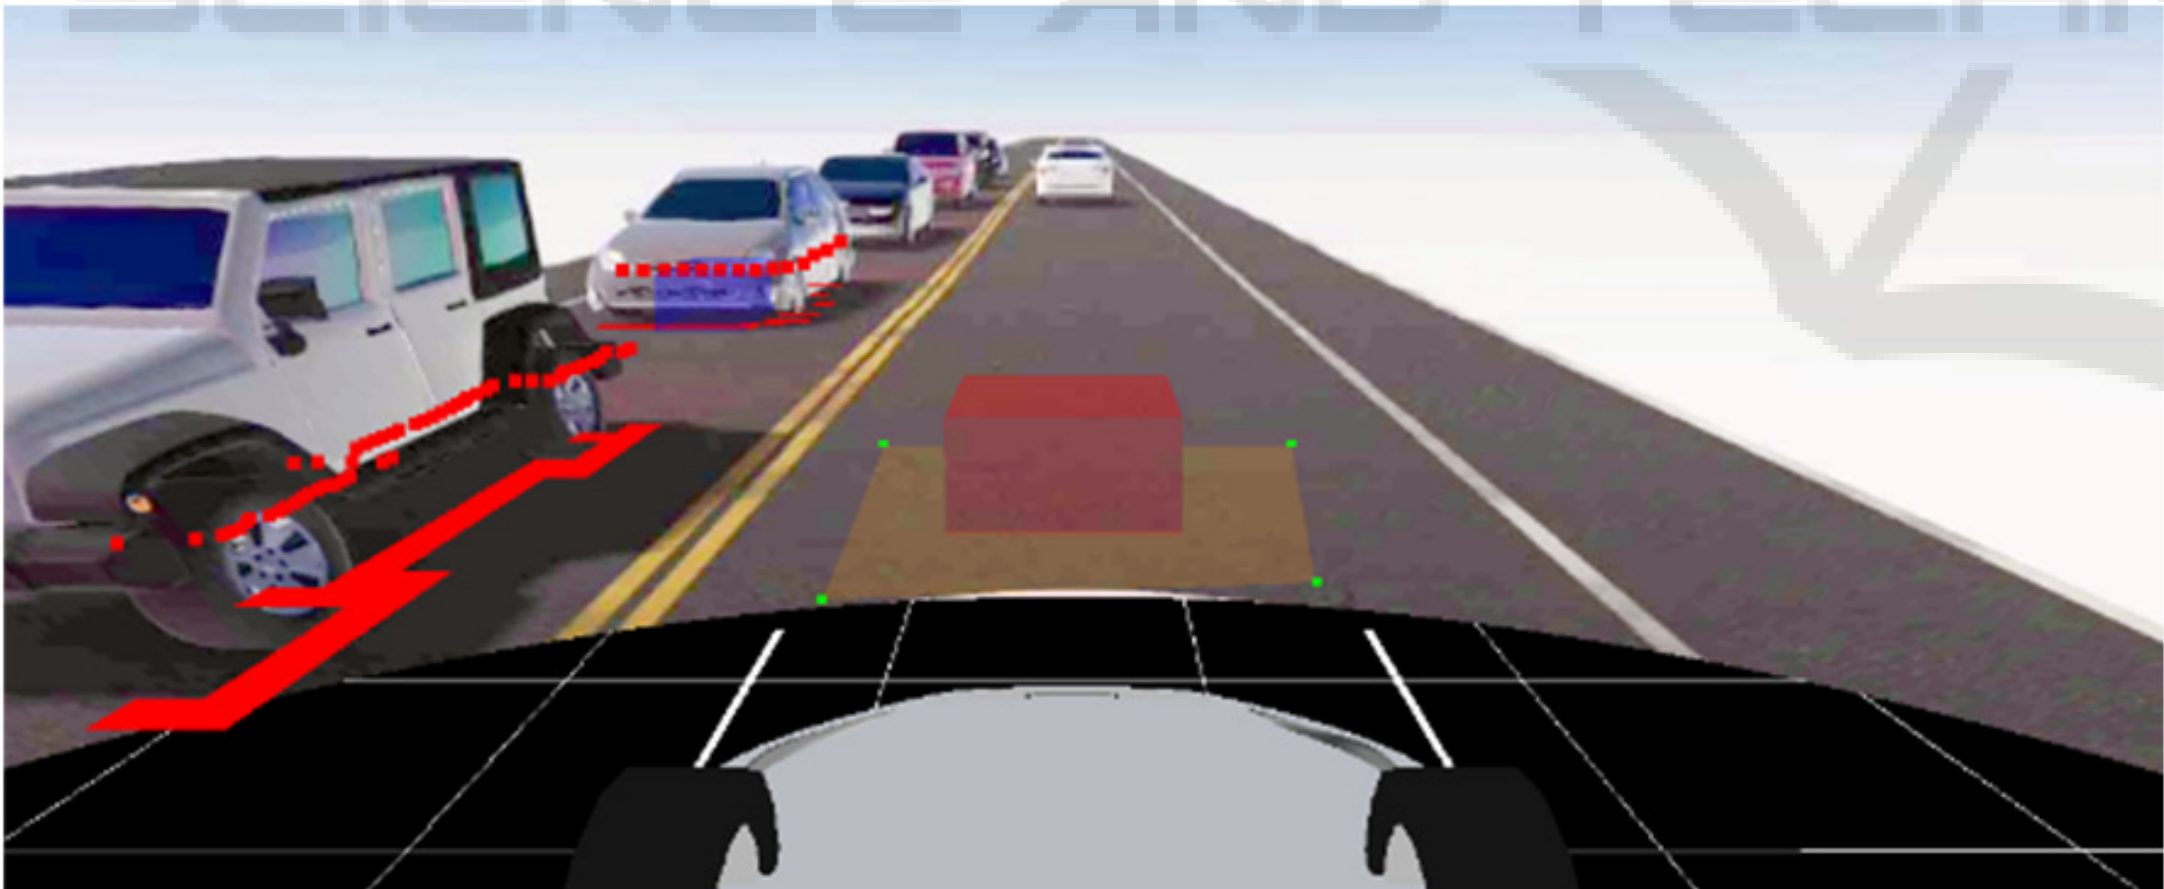
\includegraphics[width=0.8\textwidth]{figures/perceptionMod.png}
    \centering
    \caption{The interface used in the original Perception Modification paper \cite{feiler2023perception}}
    \label{fig:PerceptionMod}
\end{figure}
\paragraph{3D Space Representation} This approach involves maintaining the environmental
data in 3D space while providing methods to integrate 2D camera feeds. This can be
achieved either through projections onto basic geometric shapes, as demonstrated by
Feiler and Diermeyer \cite{Feiler2021ThePM}, and shown in the Figure \ref{fig:PerceptionMod}, or through a comprehensive 3D reconstruction of the surroundings using camera and depth data
. While geometric projection methods offer simplicity, they often encounter issues with collision of perception data points
that do not align with the projected locations. The creation of accurate 3D reconstructions, though more challenging to implement,
provides a more complete and spatially accurate representation of the environment. We will refer to this
comprehensive approach as the \emph{Integrated View} throughout this thesis, as it offers the most promising solution for
combining both raw sensor data and perception outputs in a unified, spatially coherent representation. We will explore
two approaches for implementing this Integrated View. The first approach involves using \ac{NeRF} to rendering
realistic 3D reconstructions of the environment. The second approach focuses on depth completion techniques to fuse the sensory data
to have a more complete 3D representation of the environment.

\subsection{NeRF-based rendering methods}
\ac{NeRF}, first introduced by Mildenhall et al. \cite{mildenhall2020nerf}, represent scenes as continuous volumetric functions using neural networks. A ac{NeRF} takes a 5D input coordinate (the spatial location $(x,y,z)$ and viewing direction $(\theta,\phi)$) and outputs the volume density and view-dependent emitted radiance at that spatial location. This allows photorealistic novel view synthesis by optimizing the neural network using input images with known camera poses.

In the context of autonomous driving, ac{NeRF} have been particularly effective for static perception tasks such as map construction due to their inherent property of multi-view consistency. Multiple works have applied ac{NeRF} to automotive data, focusing initially on static scenes where the environment remains unchanged \cite{snerf2023}. These approaches typically employ anti-aliased positional embeddings to handle scale variations essential for large-scale scenes.

However, autonomous driving scenarios inherently involve dynamic objects, presenting significant challenges for traditional ac{NeRF} approaches. Recent works have proposed methods to handle dynamic scenes to address this limitation. NVIDIA's EmerNeRF introduces a self-supervised approach that decomposes scenes into static, dynamic, and flow fields \cite{yang2023emernerf}. This decomposition emerges from self-supervision, enabling the model to learn from general, in-the-wild data sources without requiring ground truth annotations or external models for dynamic object segmentation.

Similarly, Wayve's PRISM-1 significantly advances handling dynamic urban environments \cite{prism2024wayve}. It can capture complex scenes with multiple moving elements, including pedestrians, cyclists, and other vehicles while accounting for dynamic lighting conditions such as blinking traffic and brake lights. The system learns to separate static from dynamic elements in a self-supervised manner and implicitly tracks movements in the scene, matching them with the 3D geometry.

When considering ac{NeRF}-based methods for our Integrated View approach, several factors must be evaluated:

\begin{table}[h!]
    \centering
    \begin{tabular}{|p{7cm}|p{7cm}|}
    \hline
    \textbf{Advantages} & \textbf{Limitations} \\ \hline
    High-fidelity photorealistic reconstructions & Significant computational resources are required for training and rendering \\ \hline
    Comprehensive representation of both static and dynamic elements & Challenges in handling highly dynamic environments with rapid changes \\ \hline
    Natural handling of multi-view consistency & Need for precise camera pose information and multiple viewpoints \\ \hline
    \end{tabular}
    \caption{Comparison of Advantages and Limitations}
    \label{table:advantages_limitations}
\end{table}

These characteristics make ac{NeRF}-based methods a promising but challenging candidate for real-time teleoperation interfaces. While they offer superior visual quality and spatial consistency, their computational demands and real-time performance limitations must be carefully considered for practical applications. It is important to note that it is a novel approach that has rapidly improved in recent years.

\subsection{Depth Completion}

Depth completion addresses converting sparse and irregular depth data into dense, regular depth information. This process is particularly relevant for \acp{AV}, where \ac{LiDAR} sensors provide accurate but sparse 3D measurements. Having complete depth information enables precise scene reconstruction, as the dense depth map allows for accurate projection of camera images onto the 3D space, creating a comprehensive view of the environment \cite{tang2023comprehensive}.

The KITTI depth completion benchmark has become the standard evaluation platform for these methods \cite{uhrig2017sparsity}, providing a dataset of over 93,000 depth maps with corresponding raw \ac{LiDAR} scans and RGB images. The benchmark evaluates methods using metrics such as \ac{iRMSE} and \ac{iMAE} to assess performance against ground truth data.

Recent advances in depth completion have explored various learning approaches. Supervised methods like GuideNet have demonstrated superior performance by effectively fusing image features at different encoder stages with sparse depth features \cite{tang2023guidenet}. The \ac{CSPN} achieves high accuracy with relatively fast runtime, making it suitable for real-time applications \cite{cheng2020cspn}. These supervised approaches, however, heavily rely on ground truth data, which can be costly and challenging to obtain in practical applications.

Self-supervised and unsupervised methods have emerged as promising alternatives that eliminate the dependence on ground truth data. Wong et al. introduced a self-supervised approach that leverages visual inertial odometry to complete depth maps without explicit supervision \cite{wong2020unsupervised}. Recent work by Li et al. explores using 3D perceptual features and multi-view geometry consistency to achieve high-precision depth completion without ground truth data \cite{li2023self}. However, the accuracy remains slightly inferior to supervised methods.

Several factors warrant consideration when considering depth completion for our Integrated View approach. The method provides accurate dense depth information and enables precise 3D scene reconstruction while being computationally more efficient than ac{NeRF}-based methods. Some implementations achieve real-time performance, making them suitable for teleoperation applications. However, the approach faces challenges such as dependence on \ac{LiDAR} sparsity patterns and potential struggles in areas with high occlusion. Additionally, the method requires careful sensor calibration and synchronization to ensure accurate fusion of \ac{LiDAR} and camera data.

These characteristics make depth completion a promising approach for real-time teleoperation interfaces, mainly when computational efficiency is a priority. Generating dense, accurate depth maps in real time provides a solid foundation for creating comprehensive environmental visualizations for teleoperators.

\section{User Experience and Interface Design for \acp{AV}}
The design of effective user interfaces for \acp{AV} represents a critical challenge in the development of safe and reliable autonomous systems. As vehicles become increasingly automated, the interaction between humans and autonomous systems becomes more complex, particularly in scenarios requiring human intervention \cite{Kettwich}. While the ultimate goal of \acp{AV} is to minimize human involvement, research has shown that human operators will still be required for handling edge cases and complex scenarios that exceed the vehicle's autonomous capabilities \cite{mutzenich2021updating}.
\subsection{Human-Machine Interaction in \acp{AV}}
\ac{HMI} in \acp{AV} focuses on creating interfaces that facilitate effective communication between the operator and the vehicle's systems. The primary goal is to ensure safe operation while maintaining an accessible user experience. This is particularly challenging in teleoperation scenarios, where operators must process complex information from multiple sources while maintaining high levels of \ac{SA} \cite{Georg}.
Modern HMI systems incorporate multiple interaction modalities to enhance operator performance and safety. Visual interfaces through \acp{GUI} serve as the primary information channel, while additional modalities such as auditory and haptic feedback provide complementary information \cite{kallioniemi2021enhancing}. This multi-modal approach helps distribute cognitive load across different sensory channels, potentially improving operator performance and reducing mental workload.
\subsection{User-Centered Design Principles for Vehicle Interfaces}
User-centered design principles highlight understanding user needs, expectations, and limitations while ensuring safety and performance. Following the EN ISO 9241-110 process, interface design consists of four key steps: understanding the context of use, specifying usage requirements, developing design solutions, and evaluating these solutions \cite{Georg}.

Kettwich et al. established seven critical requirements for teleoperation interfaces \cite{Kettwich}:

\begin{table}[h!]
    \centering
    \begin{tabular}{@{}p{4cm}p{10cm}@{}} % Remove padding with @{}
    \toprule
    \textbf{Category} & \textbf{Description} \\
    \midrule
    Features & The interface must provide necessary features to monitor automation, provide disturbance information, and support operators in resolving issues \\
    Information & The system must present necessary information effectively \\
    Situational Awareness & The interface must maintain high operator \ac{SA} \\
    Usability & The system must demonstrate good usability \\
    User Acceptance & The interface must achieve high user acceptance \\
    Attention & The system must effectively direct user attention to relevant information \\
    Capacity & The interface must not overwhelm the operator's mental and physical capacities \\
    \bottomrule
    \end{tabular}
    \caption{Requirements for the Interface}
    \label{table:interface_requirements}
    \end{table}
Within the scope of this thesis, we focus specifically on \ac{SA}, capacity (examined through cognitive load), and the combined aspects of features and information presentation on quantifiable aspects. While the remaining requirements (usability, user acceptance, and attention) are crucial for teleoperation interfaces, they fall outside the scope of our analysis.

Additionally, Georg et al. emphasize system-level requirements that are crucial for practical implementation \cite{Georg}:
\begin{table}[h!]
    \centering
    \begin{tabular}{@{}p{4cm}p{10cm}@{}}
    \toprule
    \textbf{Category} & \textbf{Description} \\
    \midrule
    Scalability & The system should be cost-effective and be able to efficiently handle multiple vehicles \\
    Adaptability & The interface should accommodate different vehicles and scenarios \\
    Data Management & Only necessary sensor data should be transmitted to minimize bandwidth usage \\
    Multi-modal Support & The system should support both conventional displays and head-mounted displays \\
    \bottomrule
    \end{tabular}
    \caption{System Requirements for Scalability and Adaptability}
    \label{table:scalability_adaptability}
    \end{table}
These requirements were also considered throughout the development phase and are discussed in the later sections.

After the requirements phase, user-centered design process involves:

\paragraph{Design Solution Development:} Creating interfaces that meet the specified requirements through iterative prototyping and refinement. This includes implementing visualization methods that effectively combine sensor data and perception outputs.
This aspect of the process is discussed within Chapter \ref{chapter:methodology}.
\paragraph{Evaluation:} Testing the design solutions against the requirements through user studies and expert evaluations. This involves measuring \ac{SA}, cognitive load, and task performance using standardized metrics and assessment tools. And This part of the process is introduced in Section \ref{section:evaluationmethods} and analyzed in more detail in Chapter \ref{chapter:userstudy}.

This systematic approach ensures that the resulting interface design meets technical requirements and effectively supports operator needs and capabilities in teleoperation scenarios.


\section{Evaluation Methods}\label{section:evaluationmethods}
The evaluation of teleoperation interfaces requires a systematic approach to measure operator performance, \ac{SA}, and cognitive load. This section discusses various evaluation methods, focusing on \ac{SA}, cognitive load and interface performance evaluations.
\subsection{Situational Awareness in Teleoperation}\label{subsection:situationawareness}
As discussed in Section \ref{subsection:humanfactors}, \ac{SA} is critical in teleoperation scenarios, mainly due to the physical separation between the operator and the vehicle. Operators rely entirely on sensor data and interface representations to understand the remote environment, making the quality and presentation of this information crucial for effective operation \cite{Gnatzig}. As Endsley explains, "Even the best-trained decision makers will make the wrong decisions if they have inaccurate or incomplete SA" \cite{endsley1995toward}.

Two prominent methods are commonly used to evaluate \ac{SA} in teleoperation tasks: the \ac{SAGAT} and the \ac{SART}. \ac{SAGAT}, developed by Endsley \cite{endsley1988sagat}, is an objective measure that involves freezing a simulation at random intervals and querying operators about their perception and understanding of the situation. During these pauses, displays are blanked, and operators are asked specific questions about elements in the environment, such as object locations or potential risks \cite{endsley2000direct}. This method allows for detailed assessment across all three levels of \ac{SA}: perception (Level 1), comprehension (Level 2), and projection (Level 3).

In contrast, \ac{SART} is a subjective post-trial rating technique where operators self-assess their \ac{SA} based on factors like attention demand, attentional supply, and understanding \cite{taylor1990sart}. While \ac{SART} provides insights into operators' confidence levels, it has been criticized for measuring operator's confidence in the \ac{SA} they perceive rather than measuring the actual \ac{SA} \cite{endsley2020review}. This distinction is crucial in teleoperation tasks where overconfidence can lead to errors.

For this thesis, we adopt \ac{SAGAT} as our primary evaluation method for \ac{SA}. \ac{SAGAT} offers several advantages over \ac{SART}:
\begin{itemize}
    \item It provides objective measurements of all three levels of \ac{SA}.
    \item It has been shown to be more sensitive to experimental differences than post-trial questionnaires \cite{endsley2000direct}.
    \item It allows for detailed analysis of specific elements relevant to perception modification tasks.
\end{itemize}
By using \ac{SAGAT}, we aim to understand how different visualization approaches impact operator \ac{SA} during teleoperation.

\subsection{Cognitive Load and Information Processing}\label{subsection:cognitiveload}
Cognitive load is critical in teleoperation, as operators must process large amounts of information from multiple sources while making timely decisions. High cognitive load can impair performance, leading to slower reaction times, reduced \ac{SA}, and increased error rates \cite{Kettwich}. Conversely, underloading the operator can reduce vigilance and engagement, which may also negatively affect task performance \cite{mutzenich2021updating}. Therefore, designing interfaces that balance cognitive demands is crucial for effective teleoperation.

The \ac{NASA-TLX} is one of the most widely used tools for evaluating cognitive load in teleoperation scenarios. \ac{NASA-TLX} is a subjective workload assessment tool that measures an operator's perceived workload across six dimensions: mental demand (cognitive effort required), physical demand (physical exertion involved), temporal demand (time pressure experienced), performance (self-assessment of task success), effort (overall exertion required), and frustration (emotional stress or annoyance) \cite{hart1988development}. These dimensions provide a comprehensive understanding of the cognitive demands placed on operators during teleoperation tasks.

Compared to alternative methods for measuring cognitive load, \ac{NASA-TLX} offers several advantages. Physiological measures such as heart rate variability or pupil dilation provide objective data but require specialized equipment and are sensitive to external factors like stress or fatigue \cite{wickens2008multiple}. Secondary task performance methods involve measuring performance on a secondary task while completing the primary task, offering indirect insights into cognitive load but potentially interfering with the primary task. In contrast, \ac{NASA-TLX} is simple to administer and captures multiple workload dimensions without requiring additional hardware or introducing interference.

While \ac{NASA-TLX} has traditionally been used in its full form with weighted scores for each dimension, simplified versions have been developed to reduce the time required for administration and analysis \cite{hart2006nasa}. For this thesis, we adopt the simplified, unweighted version of \ac{NASA-TLX} to streamline its integration into our user studies while retaining its ability to capture critical aspects of cognitive workload. This approach aligns with the practical constraints of teleoperation scenarios and ensures minimal disruption to operator tasks during evaluations.

Using \ac{NASA-TLX} as our primary tool for assessing cognitive load, we aim to gain valuable insights into how different visualization approaches impact operator mental workload in perception modification tasks
\subsection{Feature and Information Evaluation}
In evaluating the features and information presentation of teleoperation interfaces, we adopt a subjective approach that involves gathering insights from users with expertise in autonomous driving. This approach ensures that the evaluation is grounded in practical experience and industry knowledge, providing valuable feedback on the completeness and effectiveness of the interface features.

Kettwich et al. demonstrated the value of expert evaluations in their study of teleoperation interfaces for highly automated shuttles, where control center professionals assessed the interface's usability, \ac{SA}, and feature completeness \cite{Kettwich}. Similarly, Georg et al. emphasize that domain experts are crucial for evaluating teleoperation systems to ensure that the design meets real-world operational needs \cite{Georg}.

\acp{KPI} for evaluating teleoperation interfaces include feature completeness, information accessibility, and system responsiveness \cite{Brecht}. These \acp{KPI} help ensure that the interface provides all necessary features for effective teleoperation, including monitoring automation, providing disturbance information, and supporting operators in resolving issues.

\section{Summary}
The literature review has explored various aspects of teleoperation interfaces for \acp{AV}, from fundamental concepts to specific visualization approaches. This comprehensive analysis reveals the critical role of effective \acp{HMI} in ensuring safe and efficient teleoperation, particularly for perception modification tasks.
\subsection{Requirements}

The requirements for the visualization interface were derived through a comprehensive analysis of the literature and existing approaches, as outlined in earlier sections of this thesis. The requirements stem from three main sources:

First, the critical requirements for teleoperation interfaces established by Kettwich, et al. \cite{Kettwich} provide the foundation for our interface design requirements, as summarized in Table \ref{table:interface_requirements}. These requirements ensure that the interface effectively supports teleoperation tasks while maintaining usability and safety.

Second, the system-level requirements defined by Georg, et al. \cite{Georg}. address practical implementation considerations, as shown in Table \ref{table:scalability_adaptability}. These requirements were instrumental in shaping our technical approach and ensuring system scalability.

Third, our analysis of existing visualization approaches and teleoperation challenges informed additional requirements specific to perception modification tasks. This includes insights from studies on \ac{SA} in teleoperation [Section \ref{subsection:situationawareness}], cognitive load management [Section \ref{subsection:cognitiveload}], and the technical challenges of integrating multi-sensor data [Section \ref{subsection:challengesmultisensor}].

The synthesis of these sources led to a comprehensive set of requirements categorized into four key areas: \ac{SA}, Cognitive Load, Features \& Information, and Technical considerations. These requirements are summarized in Table \ref{table:requirements}, which serves as the primary reference for our interface development and evaluation process.

By synthesizing findings from these sections and visual references, the resulting requirements ensure that the interface design aligns with both theoretical insights and practical considerations for teleoperation tasks.
\newcounter{reqcounter}
\begin{table}[h!]
    \centering
    \begin{tabular}{@{}p{4cm}p{10cm}@{}}
    \toprule
    \textbf{Category} & \textbf{Requirement Description} \\
    \midrule
    \textbf{Situational Awareness} &
    \begin{enumerate}[label=\arabic*., itemsep=0pt, topsep=0pt, leftmargin=*]
        \setcounter{enumi}{\value{reqcounter}} % Resume numbering from custom counter
        \item The interface must provide comprehensive environmental perception data to enable operators to develop and maintain high \ac{SA}.
        \item Visualization methods must effectively combine multiple sensor data streams into a coherent representation.
        \setcounter{reqcounter}{\value{enumi}} % Save current counter value
    \end{enumerate} \\
    \midrule
    \textbf{Cognitive Load} &
    \begin{enumerate}[label=\arabic*., itemsep=0pt, topsep=0pt, leftmargin=*]
        \setcounter{enumi}{\value{reqcounter}} % Resume numbering from custom counter
        \item The interface must balance information presentation to avoid overwhelming operators.
        \item Visualization approaches should minimize the mental effort required for integrating different data sources.
        \setcounter{reqcounter}{\value{enumi}} % Save current counter value
    \end{enumerate} \\
    \midrule
    \textbf{Feature \& Information} &
    \begin{enumerate}[label=\arabic*., itemsep=0pt, topsep=0pt, leftmargin=*]
        \setcounter{enumi}{\value{reqcounter}} % Resume numbering from custom counter
        \item The interface must provide the necessary features for monitoring automation and perception of data.
        \item Visualization methods must effectively present both raw sensor data and processed perception outputs.
        \item The system should support perception modification tasks through intuitive interaction methods.
        \setcounter{reqcounter}{\value{enumi}} % Save current counter value
    \end{enumerate} \\
    \midrule
    \textbf{Technical} &
    \begin{enumerate}[label=\arabic*., itemsep=0pt, topsep=0pt, leftmargin=*]
        \setcounter{enumi}{\value{reqcounter}} % Resume numbering from custom counter
        \item Real-time visualization performance to support immediate operator response.
        \item Efficient data transmission to work within network bandwidth constraints.
        \item Robust handling of various environmental conditions and sensor configurations.
        \setcounter{reqcounter}{\value{enumi}} % Save current counter value
    \end{enumerate} \\
    \bottomrule
    \end{tabular}
    \caption{Requirements for the Designed \ac{HMI}}
    \label{table:requirements}
    \end{table}
These requirements will guide the development and evaluation of our visualization approaches, ensuring that the resulting interface effectively supports teleoperation tasks while maintaining high usability and performance standards.
\subsection{Research Gap}

While teleoperation has been extensively studied as a fallback solution for \acp{AV}, limited research focuses explicitly on perception modification interfaces and their effectiveness in real-world scenarios \cite{Georg}. Existing studies have primarily concentrated on direct control or remote assistance concepts, leaving a significant gap in understanding how different visualization approaches affect operator performance in perception modification tasks.

Current research lacks comprehensive user studies comparing different visualization methods for perception data presentation. Although some studies have evaluated individual aspects of teleoperation interfaces \cite{Kettwich}, there is insufficient evidence to determine which visualization approaches are most effective for perception modification tasks. This gap is particularly notable in the context of integrating multiple data streams (2D camera feeds, 3D \ac{LiDAR} data, and perception outputs) into a unified display.

This thesis addresses these gaps through two main research objectives. First, we aim to develop and evaluate an ideal implementation of our \emph{Integrated View} approach, which combines raw sensor data and perception outputs in a unified visualization. This involves investigating how different visualization techniques affect operator \ac{SA} and cognitive load. Second, we assess how closely our current implementation approaches this ideal, identifying technical limitations and areas for improvement.

Through user studies and performance evaluations, we seek to provide empirical evidence for the effectiveness of different visualization approaches in perception modification tasks. The findings will contribute to the understanding of teleoperation interface design and lay the groundwork for future research in this field, particularly in developing more advanced visualization methods and improving operator performance in perception modification tasks.



% !TeX root = ../main.tex
% Add the above to each chapter to make compiling the PDF easier in some editors.

\chapter{Methodology}\label{chapter:methodology}
This chapter details our approach to developing and evaluating visualization interfaces for perception modification tasks in teleoperation. Our methodology addresses three key aspects: interface design, implementation of the Integrated View approach, and performance optimization.

The development process follows user-centered design principles, focusing on meeting the requirements established in Section 2.7.1. We implement two distinct interfaces - the Separate View and Integrated View - to compare their effectiveness in supporting perception modification tasks. Both interfaces are built on the ToD Visual 2.0 framework, ensuring consistent baseline functionality while enabling fair comparison of their unique visualization approaches.
\section{Interface Design}
Before talking about the implementation, we first need to discuss the interface design.
We need to design both interfaces so they fit our requirements and remain implementable in a short time. Each interface must also cover the same features to avoid bias in comparisons.
We begin by discussing the \emph{Separate View} interface.



\subsection{Separate View}
The Separate View approach presents environmental perception data through two distinct windows. The first window provides the camera feed, supporting multiple camera outputs simultaneously. The second window offers a comprehensive 3D visualization of the vehicle's perception data and environmental model \cite{Kettwich}.

The 3D visualization window integrates several key components developed by El Alami \cite{yassinethesis}: The features are shown in Table \ref{table:interface_features}.

This dual-window approach allows operators to directly compare raw sensor data with the vehicle's perception outputs, facilitating the identification of potential perception errors or misclassifications \cite{Georg}. While the implementation details of these visualization features are covered in El Alami's work \cite{yassinethesis}, they form essential components of both our interface approaches and serve as the foundation for our comparative analysis.

\subsection{Integrated View}
To implement the Integrated View approach, which combines raw sensor data and perception outputs in a unified visualization, we selected Depth Completion as the primary method for creating a coherent 3D representation. This approach allows us to generate dense depth maps from sparse \ac{LiDAR} data, which can then be used to create point clouds onto which camera images are projected.

The camera configuration is crucial in this setup, as it is the primary visual information source. Research has shown that \ac{FOV} significantly impacts teleoperation performance. Studies indicate that a 200° FOV enables 40\% higher average speeds compared to 40° FOV, and a 120° FOV reduces stopped time by half compared to 40° FOV \cite{fovConsiderations}. However, wider FOVs can increase motion sickness and scene distortion. A horizontal FOV between 120 and 200 degrees provides optimal performance for teleoperation tasks \cite{fovConsiderations}. We selected a 120-degree FOV to balance performance requirements with information density and cognitive load considerations.

For video quality, we opted for 1280x720 resolution at 30 frames per second. This configuration requires 1.5 to 3 Mbit/s upstream bandwidth \cite{vdocipher2024bandwidth}, which aligns with the average network capabilities in Germany. As the camera stream represents the primary bandwidth constraint, this resolution provides the highest quality possible while maintaining reliable transmission.

The completed point cloud is a base layer for additional perception data visualization. We overlay this with the perception information from the Separate View shown in the Table \ref{table:interface_features}.

The detailed implementation of these components and the depth completion approach are discussed in Section \ref{section:integratedviewimplementation}.

\begin{table}[h!]
    \centering
    \begin{tabular}{@{}p{3cm}p{5.3cm}p{5.3cm}@{}}
    \toprule
    \textbf{Feature Category} & \textbf{Separate View} & \textbf{Integrated View} \\
    \midrule
    Visualization \par Approach & Two distinct windows: one for camera feed and another for 3D visualization of perception data. & Unified visualization combining raw sensor data and perception outputs into a single window. \\
    \midrule
    Camera Feed & Supports multiple camera outputs simultaneously in a dedicated window. & Camera images are projected onto a dense point cloud generated through depth completion. \\
    \midrule
    Point Cloud Data & Displayed in a separate 3D visualization window. & Generated using depth completion from sparse \ac{LiDAR} data and overlaid with camera projections. \\
    \midrule
    Object Detection & Color-coded bounding boxes for object detection and classification in 3D visualization. & Same as Separate View. \\
    \midrule
    Lanelet Map & Lanelet map visualization with regulatory elements in the 3D visualization window. & Same as Separate View. \\
    \midrule
    Trajectory \par Visualization & Planned trajectory visualization for the ego vehicle and prediction trajectories for other traffic participants displayed in 3D visualization. & Same as Separate View. \\
    \bottomrule
    \end{tabular}
    \caption{Comparison of Features Between Separate View and Integrated View Interfaces}
    \label{table:interface_features}
    \end{table}


\section{Integrated View Implementation}\label{section:integratedviewimplementation}

The Integrated View implementation consists of several key components that work together to create a unified visualization of environmental perception data. This section details the technical implementation of each component, starting with the fundamental camera-to-point-cloud projection and continuing through depth completion, rendering, and the complete system integration.

The pipeline for generating the integration starts with estimating a depth map of the environment using a depth completion model, creating a point cloud out of this depth map, and then projecting the camera image onto this point cloud to have a realistic rendering of the environment in the end that can be seen in Figure \ref{fig:depth_completion_result}. The following sections detail the implementation of each step in this pipeline.

\subsection{Camera to Point Cloud Projection}

\begin{figure}
    \centering
    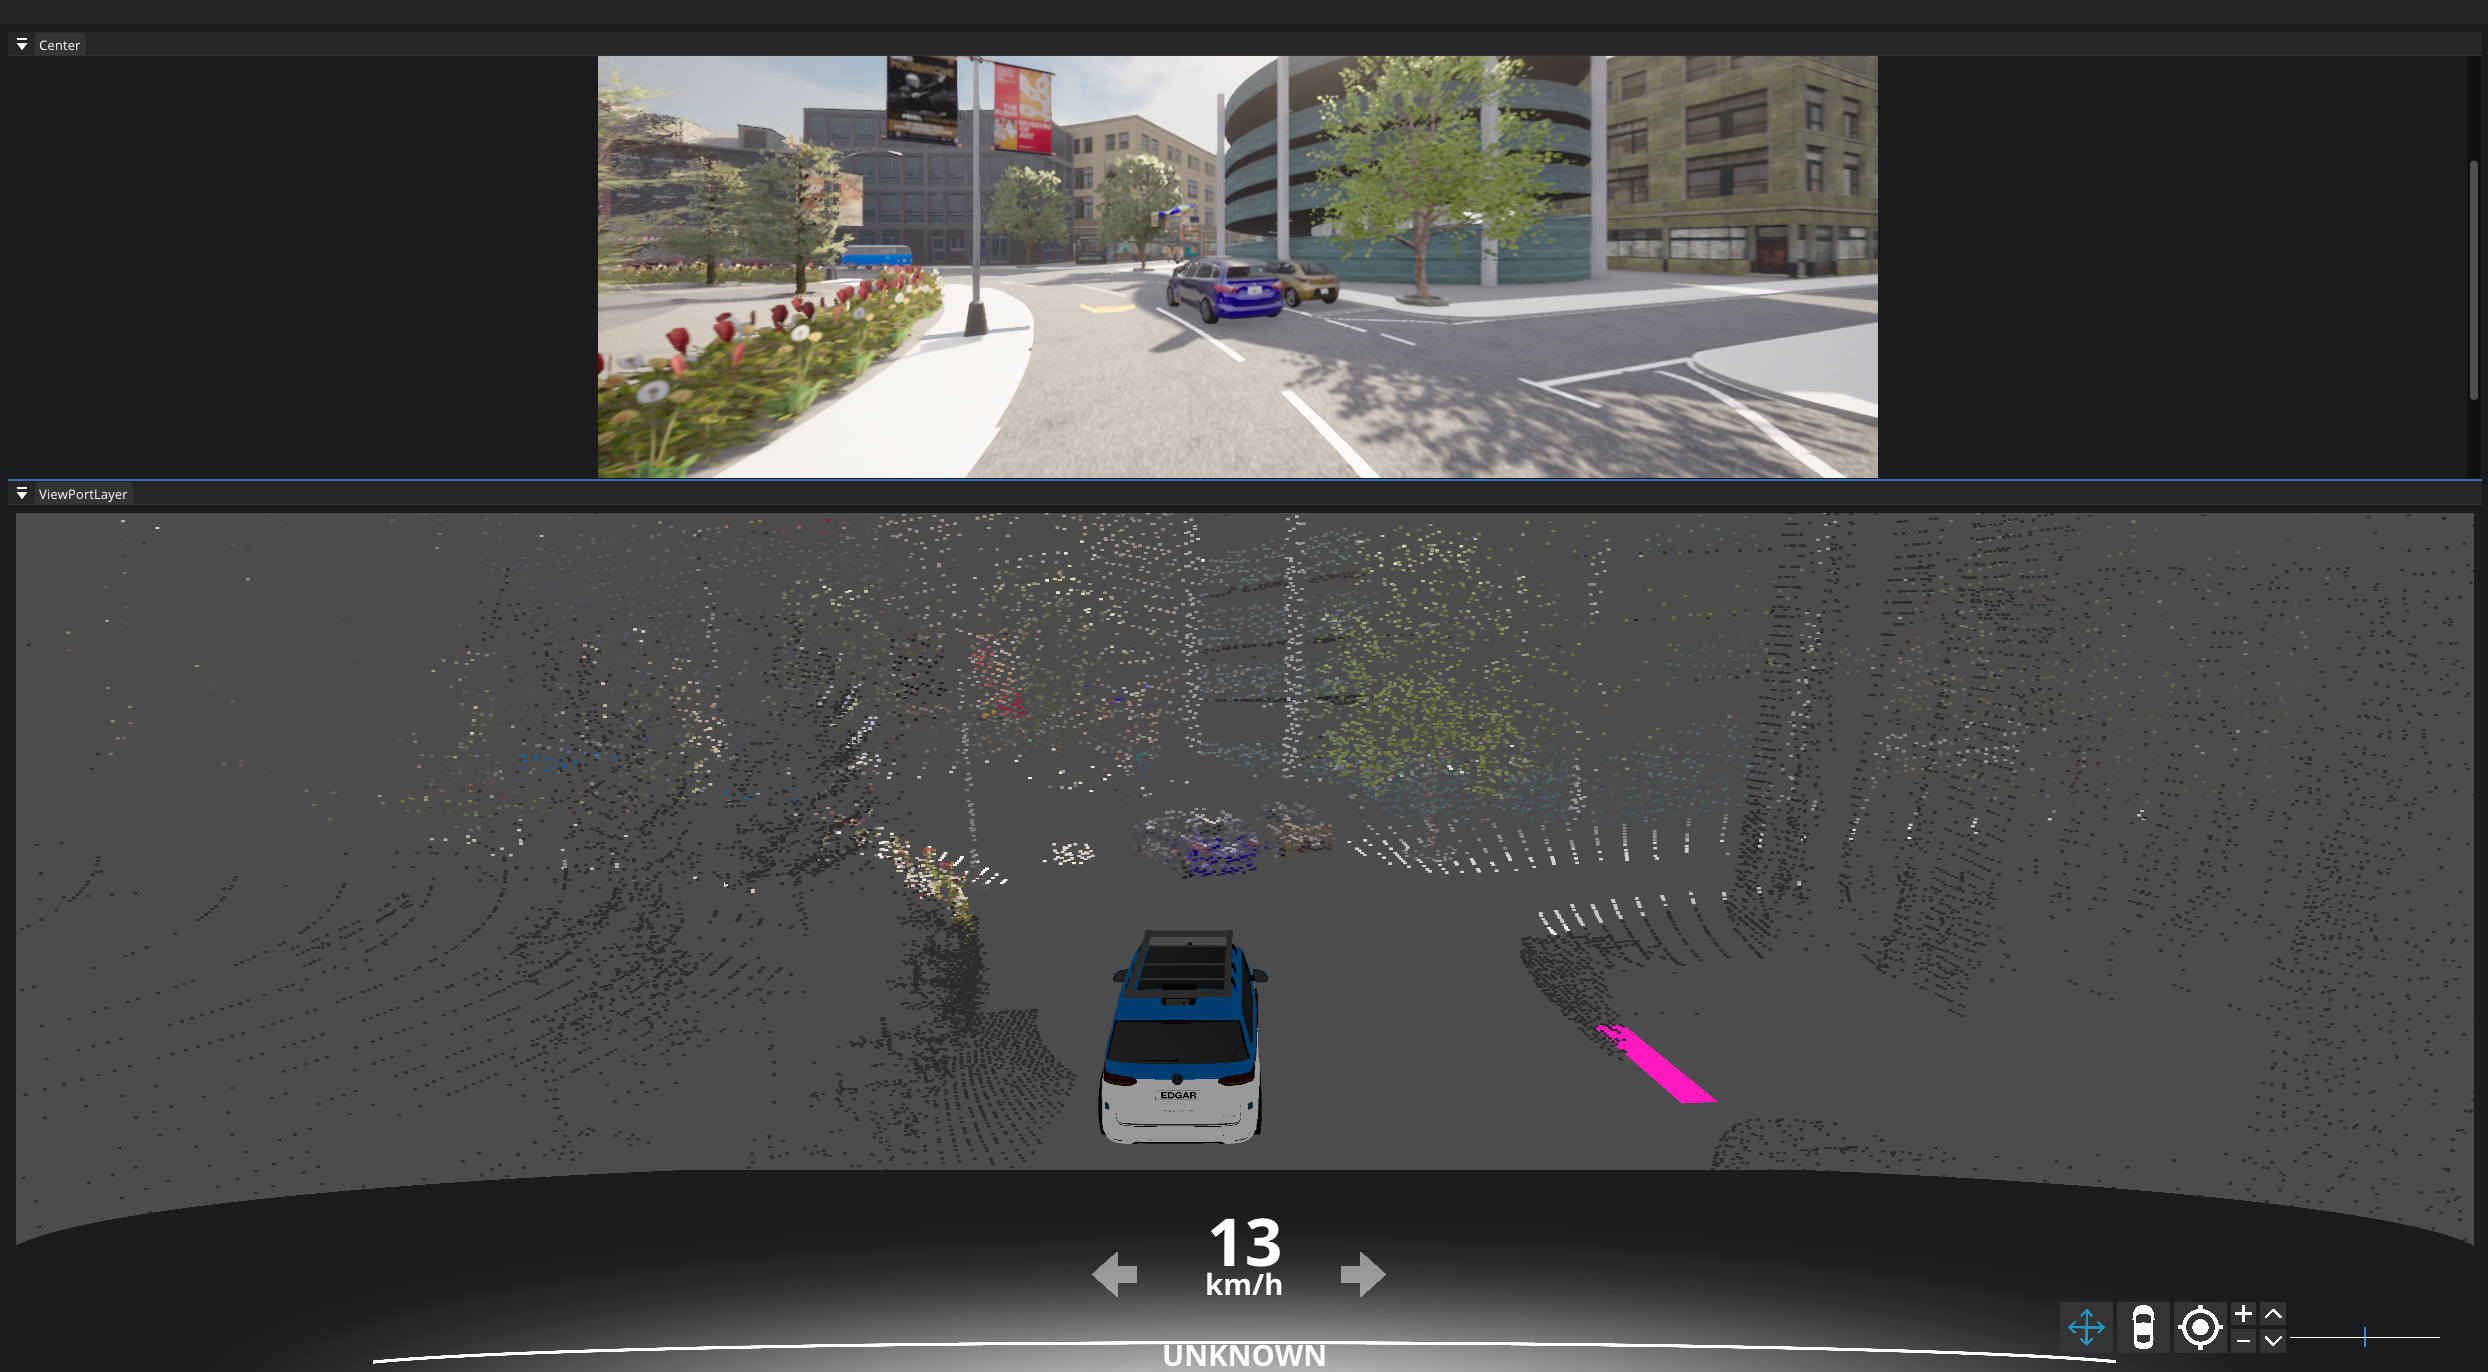
\includegraphics[width=\textwidth, trim=0 150pt 0 50pt, clip]{figures/pc.png}
    \caption{\ac{LiDAR} point cloud from the simulation colored by camera projection}
    \label{fig:camera_projection}
\end{figure}

The first step in creating our Integrated View is establishing an accurate projection between the camera image space and the 3D \ac{LiDAR} point cloud. This process involves several mathematical transformations to align the different coordinate systems and project 3D points onto the 2D image plane.

\subsubsection{Coordinate System Transformations}

To project a 3D point from the \ac{LiDAR} coordinate system to the camera image plane, we perform the following sequence of transformations:
\begin{enumerate}
    \item Transform the point from \ac{LiDAR} coordinates to camera coordinates using extrinsic parameters.
    \item Project the transformed point onto the camera's image plane using intrinsic parameters.
    \item Apply the color information from the projected pixel back to the 3D point.
\end{enumerate}

The mathematical representation of this process can be expressed as:

\[
p_{\text{cam}} = T_{\text{cam}}^{\text{lidar}} \cdot p_{\text{lidar}}
\]

where \( T_{\text{cam}}^{\text{lidar}} \) is the transformation matrix from LiDAR to camera coordinates, and \( p_{\text{lidar}} \) is a point in LiDAR coordinates represented in homogeneous form:

\[
p_{\text{lidar}} = \begin{bmatrix} x \\ y \\ z \\ 1 \end{bmatrix}
\]

\subsubsection{Camera Projection Model}

The projection of 3D points onto the image plane follows the pinhole camera model. Given the camera's intrinsic matrix \( K \):

\[
K = \begin{bmatrix}
f_x & 0 & c_x \\
0 & f_y & c_y \\
0 & 0 & 1
\end{bmatrix}
\]

The projection equation becomes:

\[
\begin{bmatrix} u \\ v \\ 1 \end{bmatrix} = K \begin{bmatrix} R | t \end{bmatrix} \begin{bmatrix} X \\ Y \\ Z \\ 1 \end{bmatrix}
\]

where:
\begin{itemize}
    \item \( (u,v) \) are the pixel coordinates in the image,
    \item \( (X,Y,Z) \) are the 3D point coordinates in camera space,
    \item \( R \) is the rotation matrix,
    \item \( t \) is the translation vector.
\end{itemize}

\subsubsection{Color Assignment}

After projection, we determine the color information for each 3D point by sampling the corresponding pixel in the camera image. To handle cases where multiple 3D points project to the same pixel, we implement a depth-based selection strategy:

\[
\text{color}(p) =
\begin{cases}
I(u,v) & \text{if } z_{\min} \leq z \leq z_{\max} \\
0 & \text{otherwise}
\end{cases}
\]

where:
\begin{itemize}
    \item \( I(u,v) \) is the image color at pixel coordinates \( (u,v) \),
    \item \( z_{\min} \) and \( z_{\max} \) define the valid depth range.
\end{itemize}

This projection process forms the foundation for our Integrated View,
enabling the combination of \ac{LiDAR} point cloud data with camera imagery as seen in the Figure \ref{fig:camera_projection}.
This critical step ensures a coherent 3D representation of the vehicle's environment.
Thus we also employed this method in the Separate View to color the raw point cloud
coming from the \ac{LiDAR} sensors.

In the next section we discuss how to populate the point cloud from a depth map. What's good about this
projection method is it being input agnostic, meaning it can be used either with a depth map point cloud,
or a raw point cloud from a \ac{LiDAR} sensor without any changes.

\subsection{Depth Cloud Rendering}

\begin{figure}
    \centering
    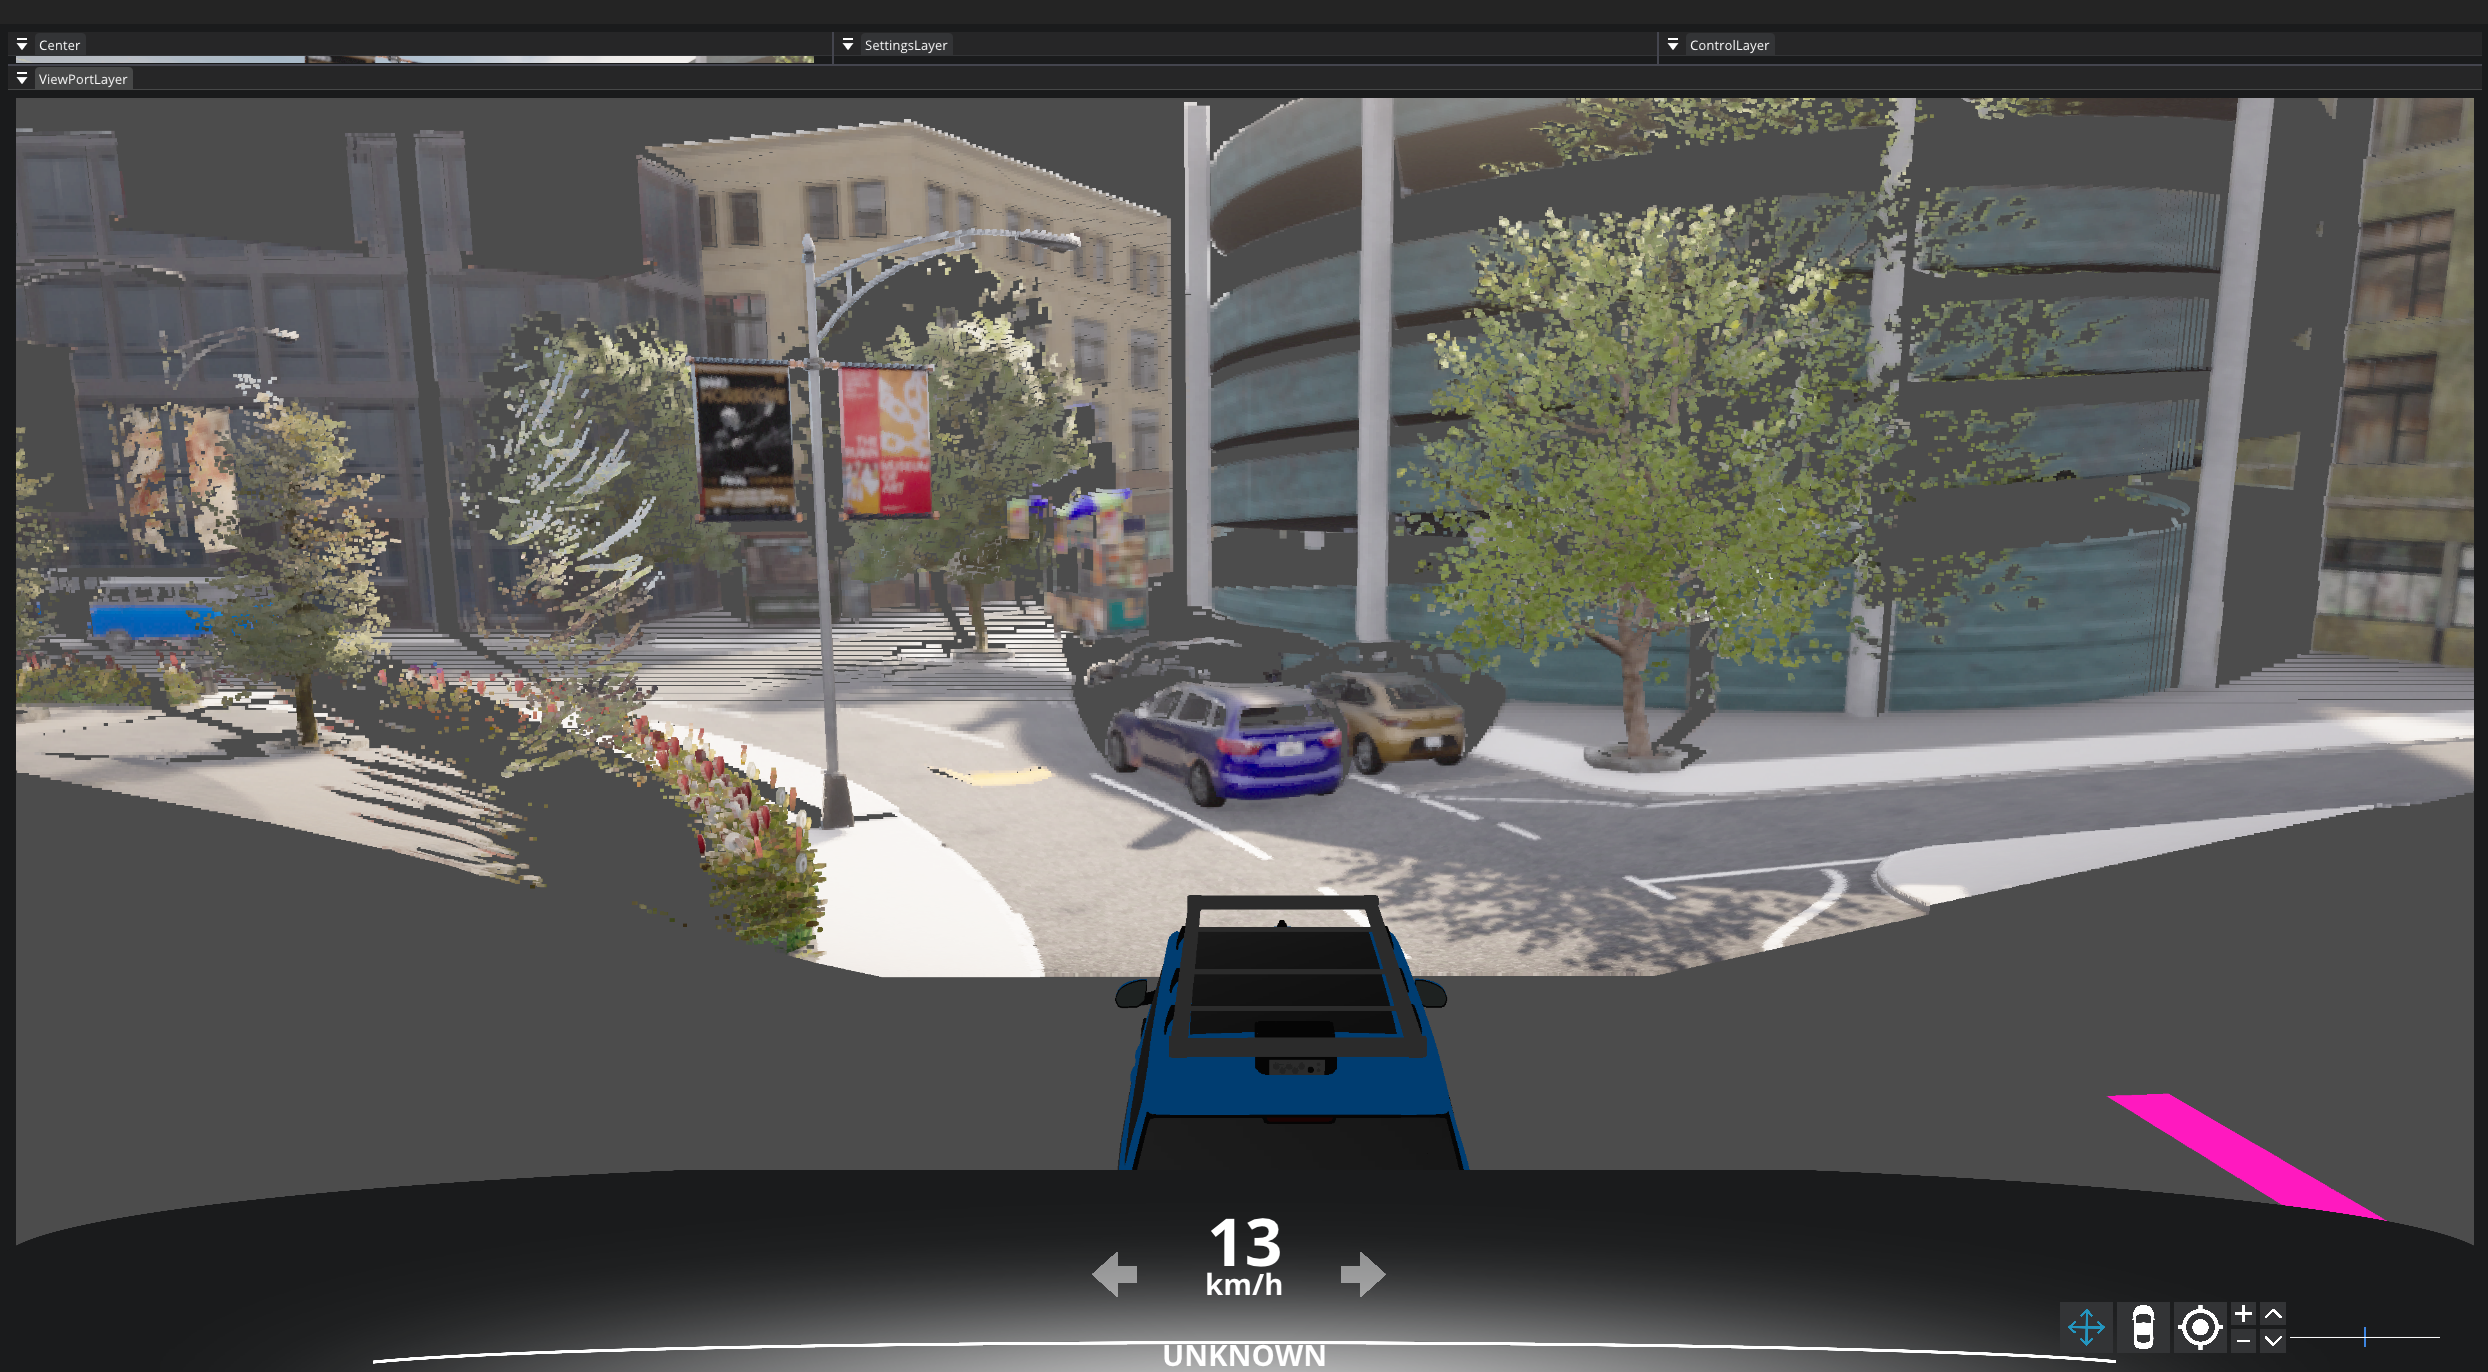
\includegraphics[width=\textwidth, trim=0 150pt 0 50pt, clip]{figures/gt.png}
    \caption{Depth cloud rendering from a the ground truth depth map}
    \label{fig:depth_cloud}
\end{figure}

Depth cloud rendering is a crucial step in creating the Integrated View, as it involves generating a 3D point cloud from a depth image. This process allows for the visualization of environmental data in a spatially accurate and intuitive format. For this implementation, we utilized the depth camera provided by the CARLA simulation environment. While CARLA's depth camera provides precise depth information in simulation as it can be seen from Figure \ref{fig:depth_cloud}. It is important to note that such sensors do not exist in real life. Real-world depth cameras, such as stereo cameras or \ac{LiDAR}-based systems, have significant limitations, including reduced accuracy under poor lighting conditions or sparse data points.

\subsubsection{Depth Camera in CARLA}

In CARLA, the depth camera generates a depth image where each pixel encodes the distance of a point in the scene from the camera plane. The depth values are stored as floating-point numbers, representing distances in meters. This simulated sensor provides an idealized output without noise or inaccuracies, making it suitable for testing visualization techniques but not representative of real-world conditions.

The transformation from a depth image to a 3D point cloud involves converting each pixel into its corresponding 3D coordinates in the camera coordinate system. This is achieved using the intrinsic parameters of the camera, which include focal lengths (\(f_x\), \(f_y\)) and principal point offsets (\(c_x\), \(c_y\)).

\subsubsection{Mathematical Transformation}

To convert a depth image into a 3D point cloud, we use the following equations:

1. For each pixel \((u, v)\) in the image:
   \[
   X = \frac{(u - c_x) \cdot d}{f_x}, \quad
   Y = \frac{(v - c_y) \cdot d}{f_y}, \quad
   Z = d
   \]
   where:
   \begin{itemize}
    \item[--] \(X, Y, Z\) are the 3D coordinates of the point in the camera coordinate system,
    \item[--] \(u, v\) are the pixel coordinates,
    \item[--] \(d\) is the depth value at pixel \((u, v)\),
    \item[--] \(f_x, f_y\) are the focal lengths of the camera,
    \item[--] \(c_x, c_y\) are the principal point offsets.
   \end{itemize}

2. Each calculated 3D point is then represented as:
   \[
   p_{\text{camera}} = \begin{bmatrix} X \\ Y \\ Z \\ 1 \end{bmatrix}
   \]

3. To integrate color information into the point cloud:
   - For each pixel \((u, v)\), retrieve its RGB values from the corresponding color image.
   - Assign these RGB values to the 3D point.

\subsubsection{Implementation Considerations}

The implementation involves iterating over each pixel in the depth image and applying the above transformation to compute its 3D coordinates. Special care is taken to handle invalid or out-of-range depth values:
- Pixels with non-finite or zero depth values are ignored.
- Depth values exceeding a predefined range (e.g., maximum sensor range) are discarded.

The final step combines these 3D points with their corresponding color information to generate a complete colored point cloud.

\subsubsection{Limitations of Real-World Depth Cameras}

Unlike CARLA's idealized depth camera, real-world depth cameras face several challenges, as summarized in Table~\ref{table:depth_camera_limitations}.

\begin{table}[h!]
\centering
\begin{tabular}{@{}p{4cm}p{10cm}@{}}
\toprule
\textbf{Limitation} & \textbf{Description} \\
\midrule
Noise and Accuracy & Stereo cameras rely on disparity calculations and can struggle with low-texture regions or poor lighting conditions. \\
\midrule
Sparse Data & \ac{LiDAR} sensors provide high-accuracy distance measurements but produce sparse point clouds that require interpolation or fusion with other sensors. \\
\midrule
Field of View & Real-world cameras often have limited fields of view compared to simulated sensors. \\
\bottomrule
\end{tabular}
\caption{Limitations of Real-World Depth Cameras}
\label{table:depth_camera_limitations}
\end{table}

These limitations highlight why CARLA's simulated depth camera is used for prototyping and testing visualization approaches but the approach cannot be used in real-world conditions.
For this reason we implemented our neural networks based depth completion method to generate a dense point cloud from sparse LiDAR data, which is explained in the next section.

Depth cloud rendering forms a foundational part of our Integrated View implementation by enabling accurate spatial visualization of environmental data. The resulting colored point cloud serves as a base layer for integrating additional perception outputs such as object detections and lanelet maps.
\subsection{Depth Completion}
As mentioned in the last section, we must rely on something other than depth cameras for long distances. The \ac{LiDAR} sensors provide accurate depth measurements, but their sparse nature limits our ability to create a comprehensive 3D visualization of the environment.
Depth completion addresses this limitation by converting sparse depth data into dense depth maps by fusing \ac{LiDAR} and camera data. This approach is particularly relevant for our Integrated View implementation, as it enables the creation of detailed, spatially accurate scene reconstructions.

For our implementation, we selected the \ac{DySPN} architecture \cite{dyspn}, which introduces a non-linear propagation model for depth completion. Figure \ref{fig:dyspn_architecture} shows that the network employs a ResNet34-UNet backbone that generates an initial depth map, affinity matrix, and a series of spatial and sequential attention maps. The key innovation of \ac{DySPN} lies in its dynamic approach to spatial propagation - unlike previous methods \cite{cheng2020cspn} that use fixed affinity matrices, \ac{DySPN} adaptively adjusts the affinity weights during propagation through attention mechanisms.

\begin{figure}
    \centering
    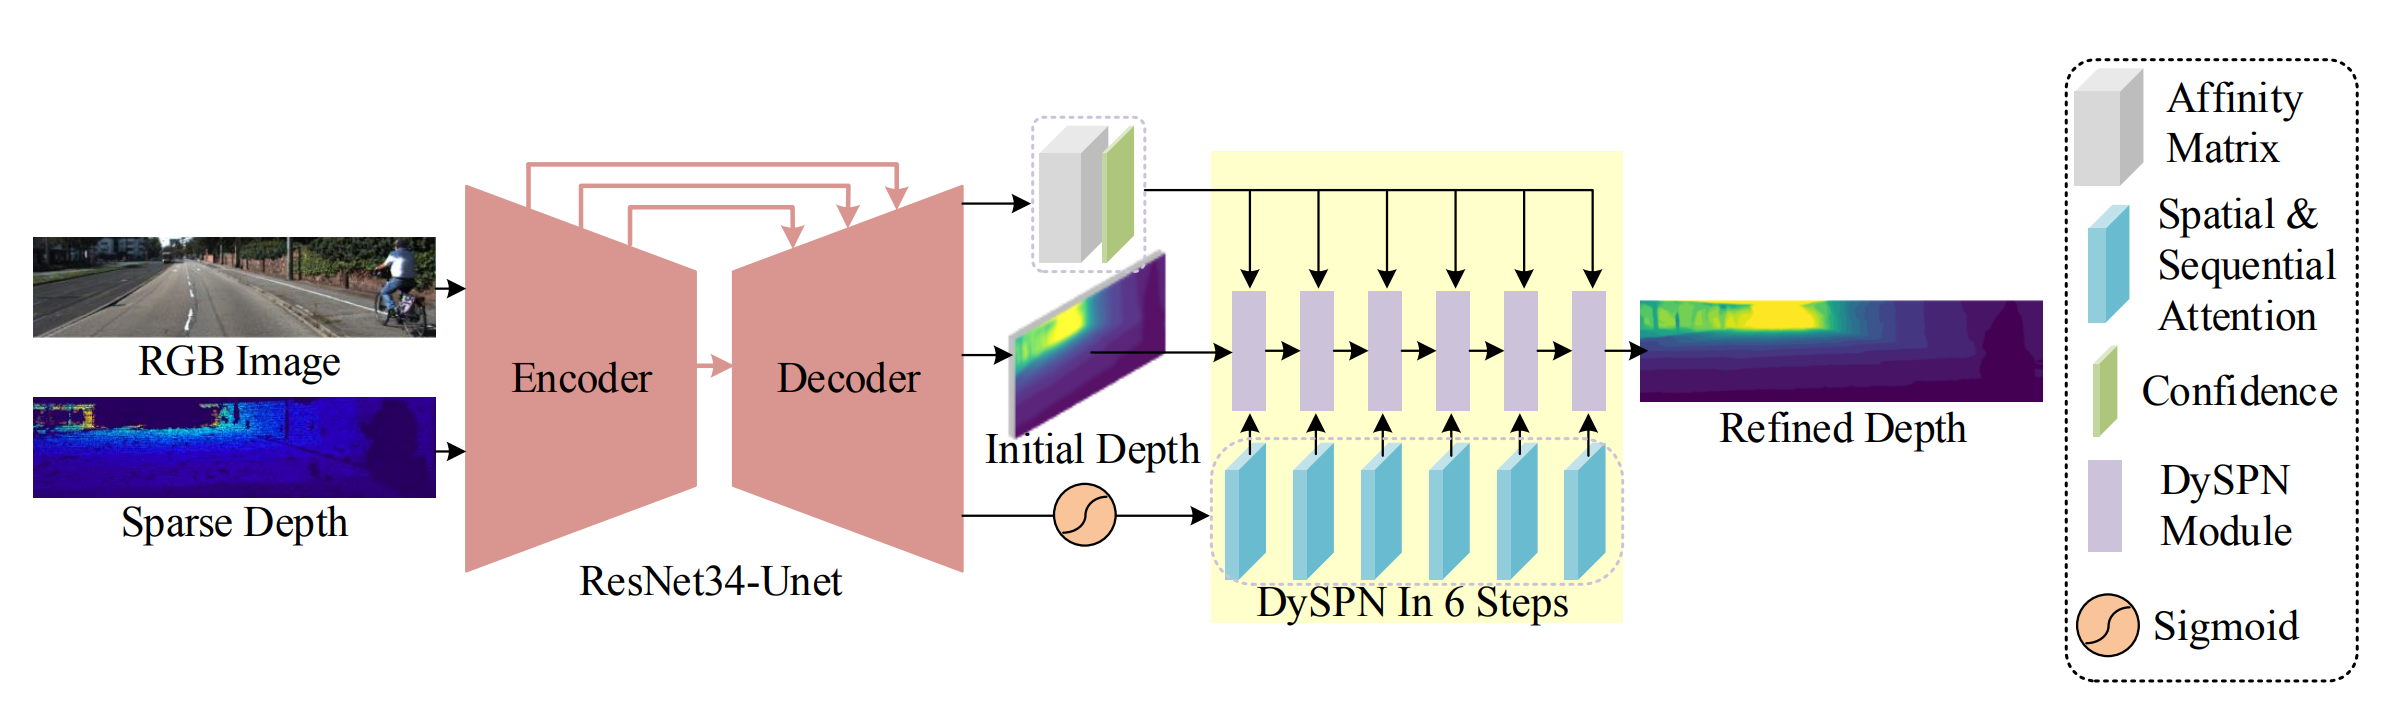
\includegraphics[width=\textwidth]{figures/dyspn.png}
    \caption{\ac{DySPN} Architecture \cite{dyspn}}
    \label{fig:dyspn_architecture}
\end{figure}

We chose \ac{DySPN} for several key reasons, as summarized in Table~\ref{table:dyspn_reasons}.

\begin{table}[h!]
\centering
\begin{tabular}{@{}p{4.5cm}p{9.3cm}@{}}
\toprule
\textbf{Reason} & \textbf{Description} \\
\midrule
Real-time Performance & The network can achieve inference in 38ms, making it suitable for teleoperation applications. \\
\midrule
Benchmark Performance & \ac{DySPN} achieves state-of-the-art results on the KITTI depth completion benchmark with an RMSE of 709.12mm. \\
\midrule
Supervised Learning  & While supervised learning typically requires extensive ground truth data, our simulation-based development environment using CARLA provides precise depth information for training. \\
\bottomrule
\end{tabular}
\caption{Key Reasons for Selecting \ac{DySPN} Architecture}
\label{table:dyspn_reasons}
\end{table}

The ability to use CARLA's precise depth camera for generating ground truth data makes this supervised approach particularly attractive. The network's architecture, which decouples neighborhood relationships based on distance and uses attention mechanisms to dynamically adjust affinities, aligns well with our goal of creating accurate depth reconstructions for teleoperation interfaces.
For our implementation, we made several modifications to adapt the network to our specific requirements. First, we adjusted the network architecture to accommodate our image resolution of 1280x720, compared to the original KITTI resolution. Second, we reimplemented certain operations to ensure compatibility with PyTorch's JIT compilation, enabling seamless deployment in our C++ production environment.

\begin{figure}
    \centering
    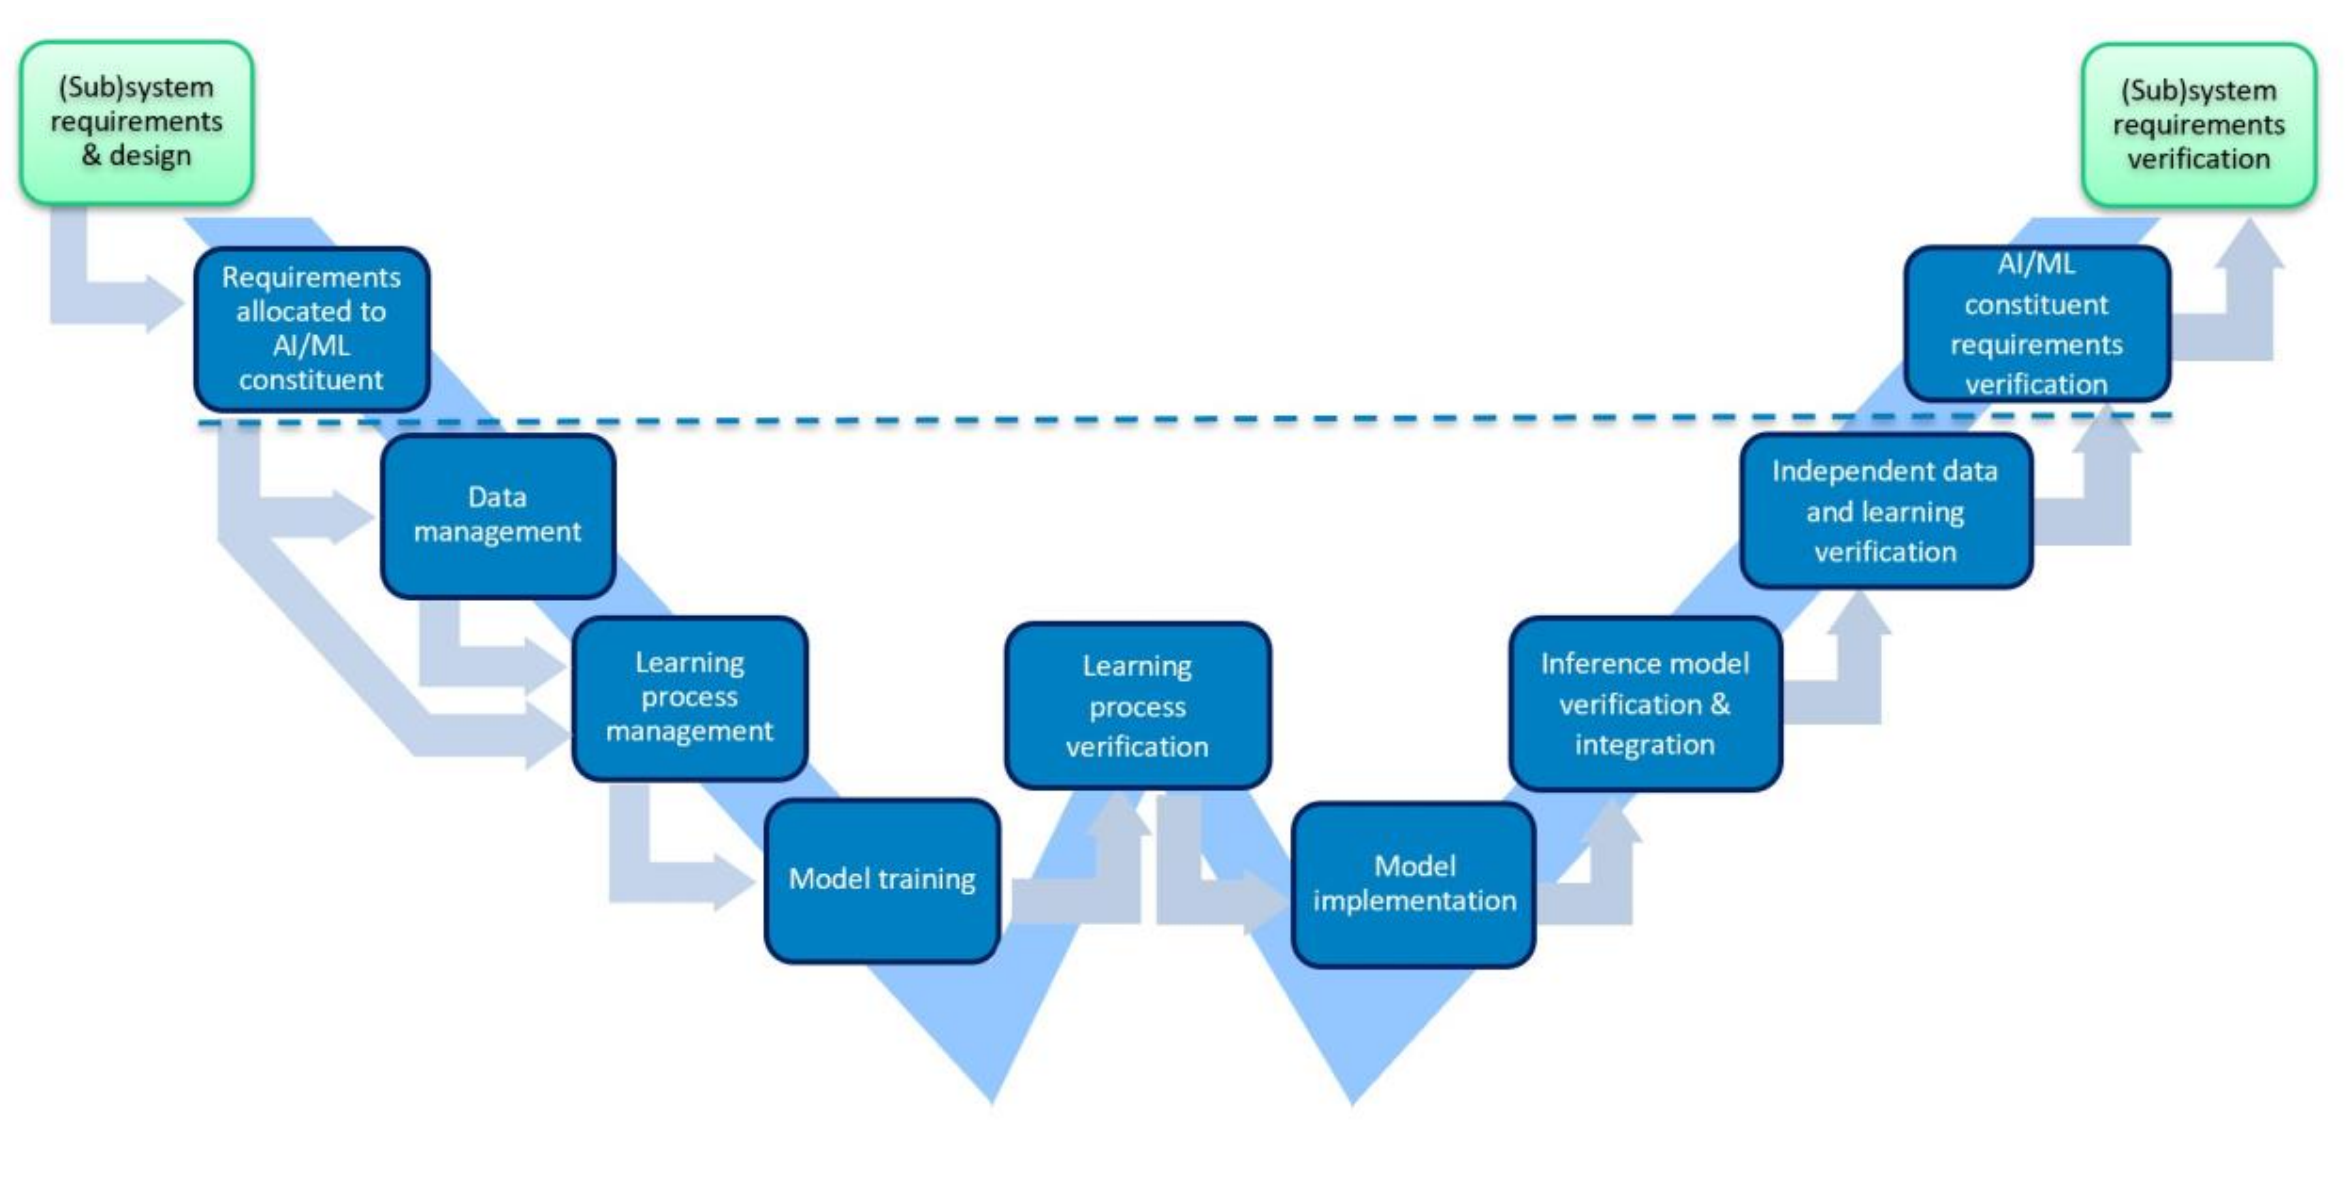
\includegraphics[width=\textwidth]{figures/wshaped.png}
    \caption{W-Shaped learning assurance from \cite{easa2024}}
    \label{fig:wshaped_learning}
\end{figure}

\subsection{W-Shaped Development Cycle}
The development approach for our depth completion model aligns with the W-shaped development cycle for learning assurance, as proposed by the European Union Aviation Safety Agency (EASA) \cite{easa2024}. This cycle provides a structured framework for developing \ac{AI} based systems.
Similar to the V-model \cite{vmodel} that is widely used for software development for safety related products, W-Shaped Development Cycle introduce an intermediate verification layer for the \ac{AI} model which creates the "W" shape as shown in the Figure \ref{fig:wshaped_learning}.
We have adapted our proof-of-concept level project to follow this method, which can be mapped to the key stages of the W-shaped cycle as shown in the Table \ref{table:wshaped_cycle}.

\begin{table}[h!]
    \centering
    \begin{tabular}{@{}p{1cm}p{13cm}@{}}
    \toprule
    \textbf{\#} & \textbf{Stage Description} \\
    \midrule
    1 & \textbf{Requirements Management:} We derived clear requirements from our literature review and identified research gaps, guiding the development of both the depth completion model and the overall interface. \\
    \midrule
    2 & \textbf{Data Management \& Verification:} We selected appropriate sensor configurations, including a 120-degree FOV camera and 1280x720 resolution at 30 fps. We utilized simulation data from CARLA for development and testing. \\
    \midrule
    3 & \textbf{Learning Process Management:} We made decisions regarding the training algorithm and architecture for depth completion, selected performance evaluation metrics (e.g., \ac{iRMSE}, \ac{iMAE}), and chose appropriate hardware and software frameworks for implementation. \\
    \midrule
    4 & \textbf{Model Training:} This phase involved the actual training of our depth completion model, separate from the main interface development. \\
    \midrule
    5 & \textbf{Learning Process Verification:} While not conducting extensive tests at this stage, we verified the learning process by evaluating the trained model's performance on test cases and iterating on the model design as needed. \\
    \midrule
    6 & \textbf{Model Implementation:} We implemented the trained depth completion model within the Integrated View interface and optimized it for real-time performance in the teleoperation context. \\
    \midrule
    7 & \textbf{Inference Model Verification:} We ensured the implemented model behaved consistently with the trained model and verified real-time performance within the interface. \\
    \bottomrule
    \end{tabular}
    \caption{Explanation of the W-shaped development cycle stages and their application to our depth completion model development}
    \label{table:wshaped_cycle}
    \end{table}

By framing our development approach within this W-shaped cycle, we demonstrate adherence to a structured methodology for developing \ac{AI}-based systems, even at a proof-of-concept level. This approach ensures consideration of key stages in \ac{AI} system development and aligns with industry best practices for learning assurance.

\subsection{Simulation Setup}

Our simulation environment integrates CARLA simulator with Autoware autonomous driving stack through the CARLA-Autoware Bridge \cite{carla_aw_bridge24}. This setup enables us to create a controlled testing environment for our visualization approaches while maintaining realistic driving scenarios.


\subsubsection{Vehicle and Sensor Configuration}
The sensor configuration aims to replicate TUM's EDGAR vehicle while maintaining computational efficiency in the simulation environment. The primary sensors are detailed in Table~\ref{table:sensor_configuration}.

\begin{table}[h!]
\centering
\begin{tabular}{@{}p{4cm}p{10cm}@{}}
\toprule
\textbf{Sensor Type} & \textbf{Specifications/Details} \\
\midrule
Frontal \ac{LiDAR}s & Two \ac{LiDAR}s with 120-meter range, positioned at the front left and right corners with 45-degree angles. \\
\midrule
\ac{LiDAR} Specifications &
20 Hz rotation rate \par
1,310,720 points per second \par
64 channels \\
\midrule
Front-facing Camera & Resolution: 1280x720, \ac{FOV}: 120°. \\
\midrule
Depth Camera & Matches the specifications of the front-facing camera. \\
\midrule
GNSS and IMU Sensors & Provides localization and orientation data. \\
\bottomrule
\end{tabular}
\caption{Sensor Configuration for Vehicle Simulation}
\label{table:sensor_configuration}
\end{table}

\subsubsection{Environment Selection}
Initial development and data collection were conducted in CARLA's Town10 environment. However, as our target user group consists of German operators, we identified potential limitations in using U.S.-based road layouts for situational awareness evaluation. To address this, we developed a custom map based on a real location in Munich, Germany. This ensures that the traffic scenarios and road layouts are familiar to our test subjects, providing more relevant data for evaluating operator performance. The details of the custom map development are discussed in Section \ref{section:mapcreationforcarla}.
\subsection{Data Collection}


To train our depth completion network, we developed a ROS application that collects synchronized sensor data from the CARLA simulation environment. The application subscribes to three main data streams: LiDAR point clouds, camera images, and depth camera outputs (which serve as ground truth). The data collection setup is illustrated in Figure \ref{fig:data_collection}.
We gathered a dataset of ${\sim}10,000$ images by manually driving through the simulation environment with dynamic weather conditions enabled. To ensure diversity in the collected data, our collection script captured sensor data at random time intervals. This approach helps prevent oversampling of similar scenes and ensures a more representative dataset.
The preprocessing pipeline transforms point cloud data into camera space using the sensor extrinsic parameters, normalizes depth values to 8-bit range (0-255) for efficient storage, and projects 3D points onto the image plane using camera intrinsics. The processed data was stored in NumPy's .npy format using 32-bit floating-point precision per pixel. This format was chosen for its efficient storage and fast loading capabilities during training, while maintaining sufficient numerical precision for depth values. The pint cloud input can be seen in Figure \ref{fig:pointcloud_input}
\begin{figure}[h]
    \centering
    \begin{subfigure}{\textwidth}
        \centering
        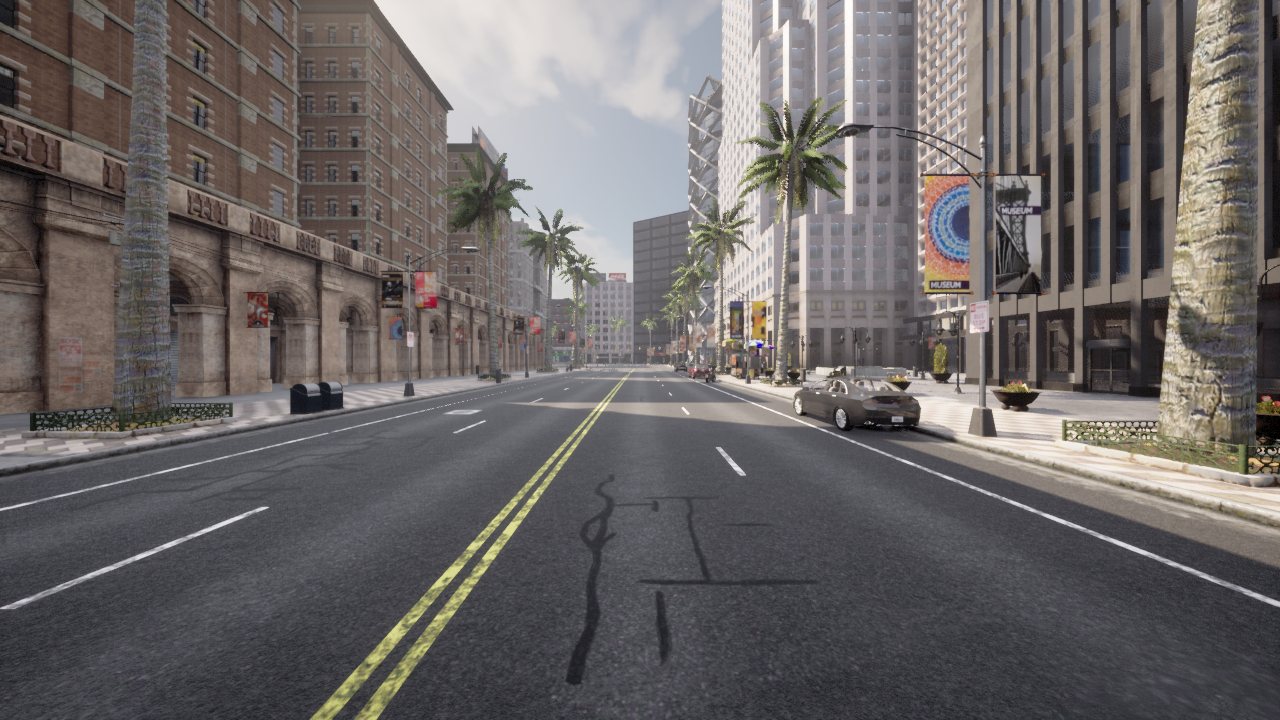
\includegraphics[width=\textwidth, trim=0 200pt 0 200pt, clip]{figures/rgb.png}
        \caption{RGB camera image from CARLA simulation}
        \label{fig:rgb_input}
    \end{subfigure}
    \begin{subfigure}{\textwidth}
        \centering
        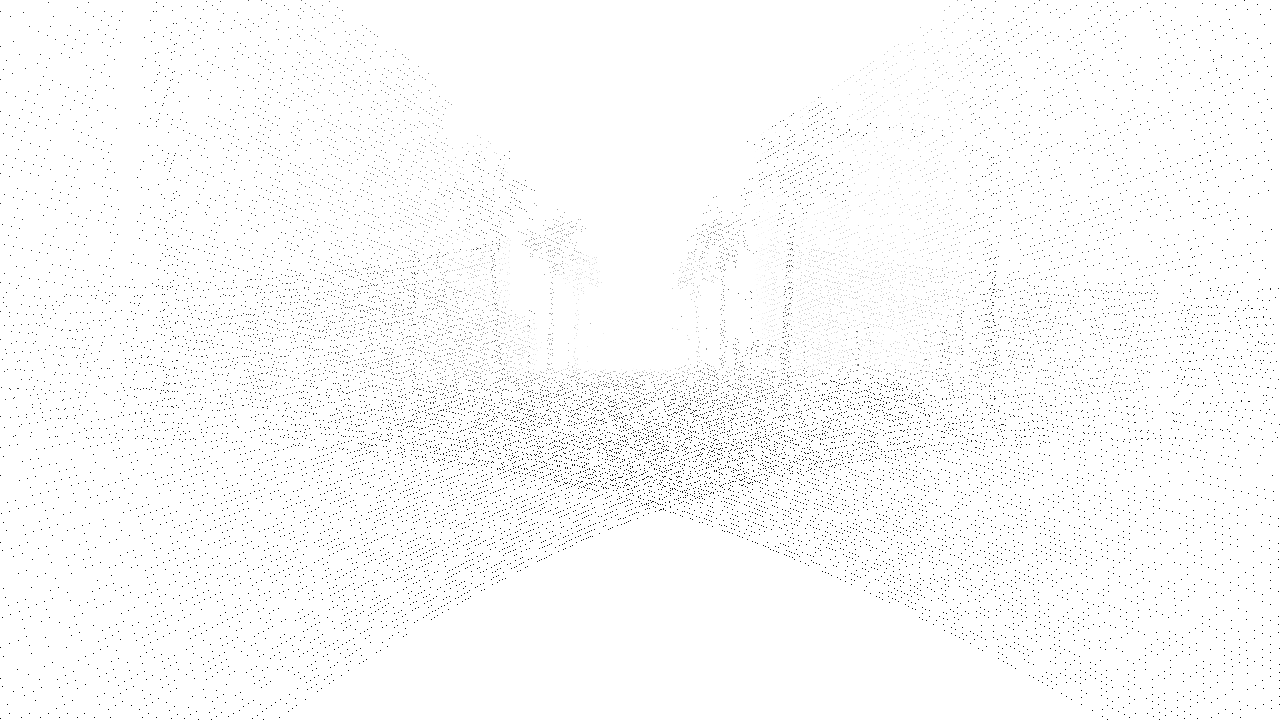
\includegraphics[width=\textwidth, trim=0 200pt 0 200pt, clip]{figures/point_cloud.png}
        \caption{Projected \ac{LiDAR} point cloud showing sparse depth information}
        \label{fig:pointcloud_input}
    \end{subfigure}
    \begin{subfigure}{\textwidth}
        \centering
        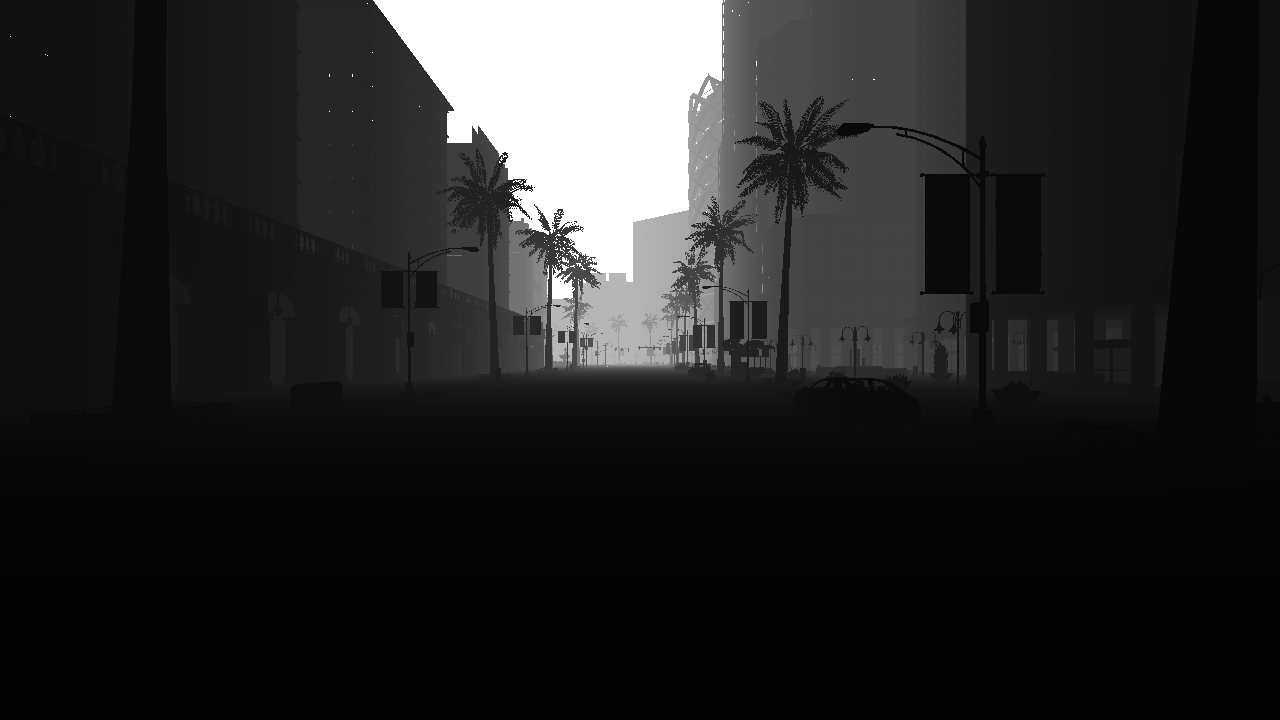
\includegraphics[width=\textwidth, trim=0 200pt 0 200pt, clip]{figures/depth_gt.png}
        \caption{Ground truth depth map from CARLA's depth camera}
        \label{fig:depth_gt}
    \end{subfigure}
    \caption{Example of collected training data showing the three input types: RGB image, sparse \ac{LiDAR} point cloud, and ground truth depth map}
    \label{fig:data_collection}
\end{figure}
\FloatBarrier

\subsection{Training}

We conducted the training on an NVIDIA RTX 4090 GPU using the AdamW optimizer, which combines the benefits of the Adam optimizer with weight decay regularization. AdamW addresses the potential interference between L2 regularization and momentum in the original Adam optimizer, making it particularly effective for \ac{DL} tasks by providing better generalization and more stable training dynamics.

Through grid search optimization, we evaluated learning rates ranging from 0.01 to 0.0001 and batch sizes of 1 and 2, with hardware limitations preventing larger batch sizes. The initial five epochs of each configuration were analyzed to assess training stability and validation loss trends. Based on these results, we selected a learning rate of 0.001 and a batch size 1 for the final training run of 100 epochs. We implemented a learning rate scheduler that reduces the learning rate when the validation loss plateaus to optimize the training process.

\begin{figure}[h]
    \centering
    \begin{subfigure}{0.48\textwidth}
        \centering
        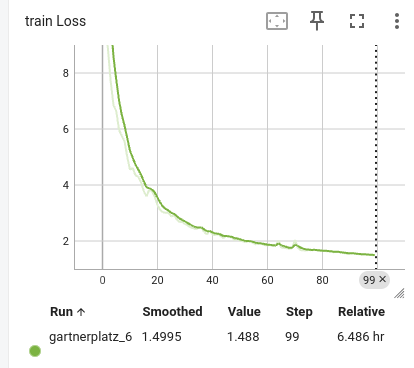
\includegraphics[width=\textwidth]{figures/train.png}
        \caption{Training loss curve}
        \label{fig:train_curve}
    \end{subfigure}
    \hfill
    \begin{subfigure}{0.48\textwidth}
        \centering
        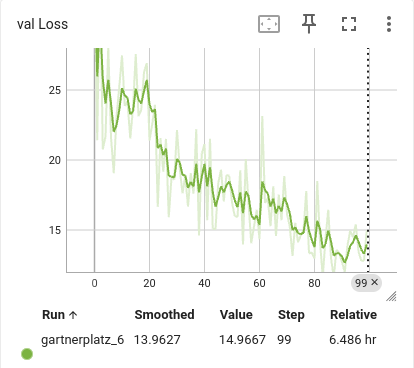
\includegraphics[width=\textwidth]{figures/validation.png}
        \caption{Validation loss curve}
        \label{fig:val_curve}
    \end{subfigure}
    \caption{Training and validation loss curves over 100 epochs}
    \label{fig:training_curves}

\end{figure}
The loss function combines three components:


\[
L_{total} = \alpha L_1 + \beta L_2 + \gamma L_{SSIM}
\]


where the \ac{SSIM} loss evaluates the perceptual quality between predicted and ground truth depth maps. SSIM considers luminance, contrast, and structural information, making it particularly effective for maintaining overall depth map consistency. The L1 and L2 losses were specifically weighted to focus on depths below 120 meters, aligning with our \ac{LiDAR}'s range:

\[
    L_{1,2} = \begin{cases}
    L_{1,2}(pred, gt) & \text{if } depth < 120m \\
    0 & \text{otherwise}
    \end{cases}
\]

The validation loss shows consistent improvement throughout training, decreasing from approximately 30 to 15 over 99 epochs. While there are noticeable oscillations in the validation curve, particularly in earlier epochs, the overall downward trend indicates successful model convergence. The final validation loss of 14.96 and smoothed curve suggest that the learning rate scheduler effectively managed the training process.


\begin{figure}[h]
    \centering
    \begin{subfigure}{\textwidth}
        \centering
        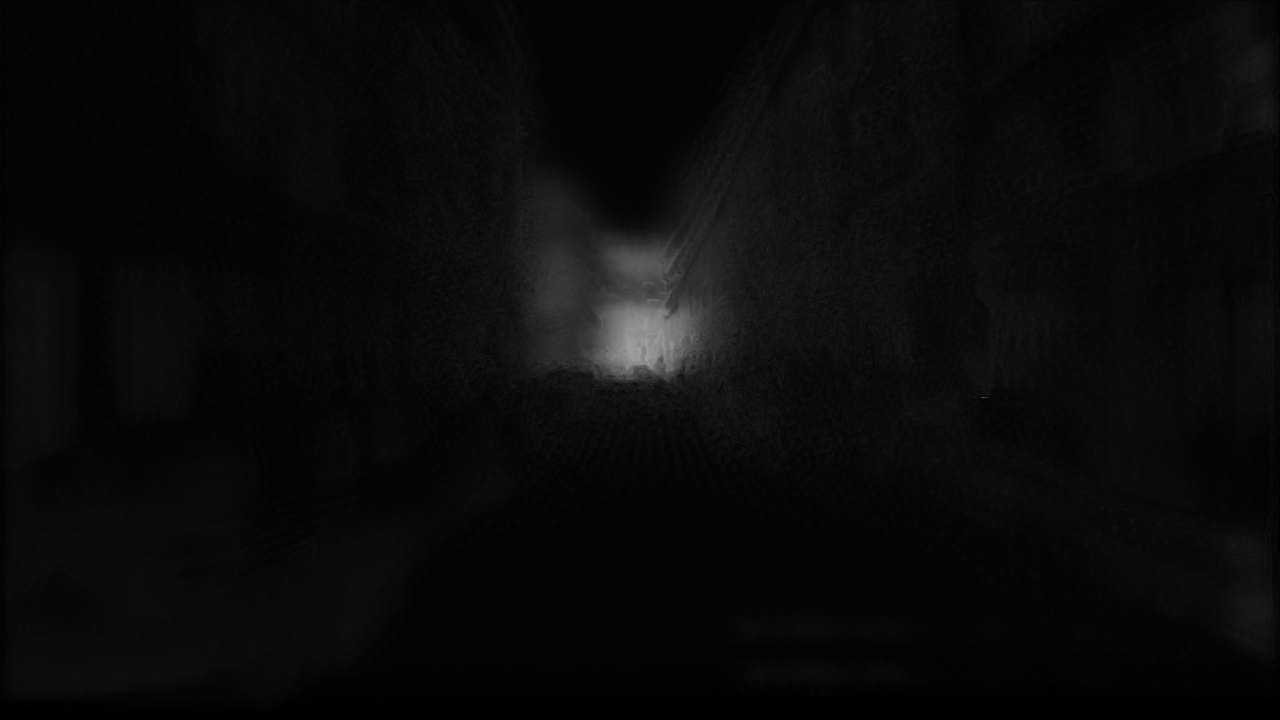
\includegraphics[width=\textwidth, trim=0 200pt 0 200pt, clip]{figures/step1.png}
        \caption{Epoch 1}
        \label{fig:epoch1}
    \end{subfigure}
    \hfill
    \begin{subfigure}{\textwidth}
        \centering
        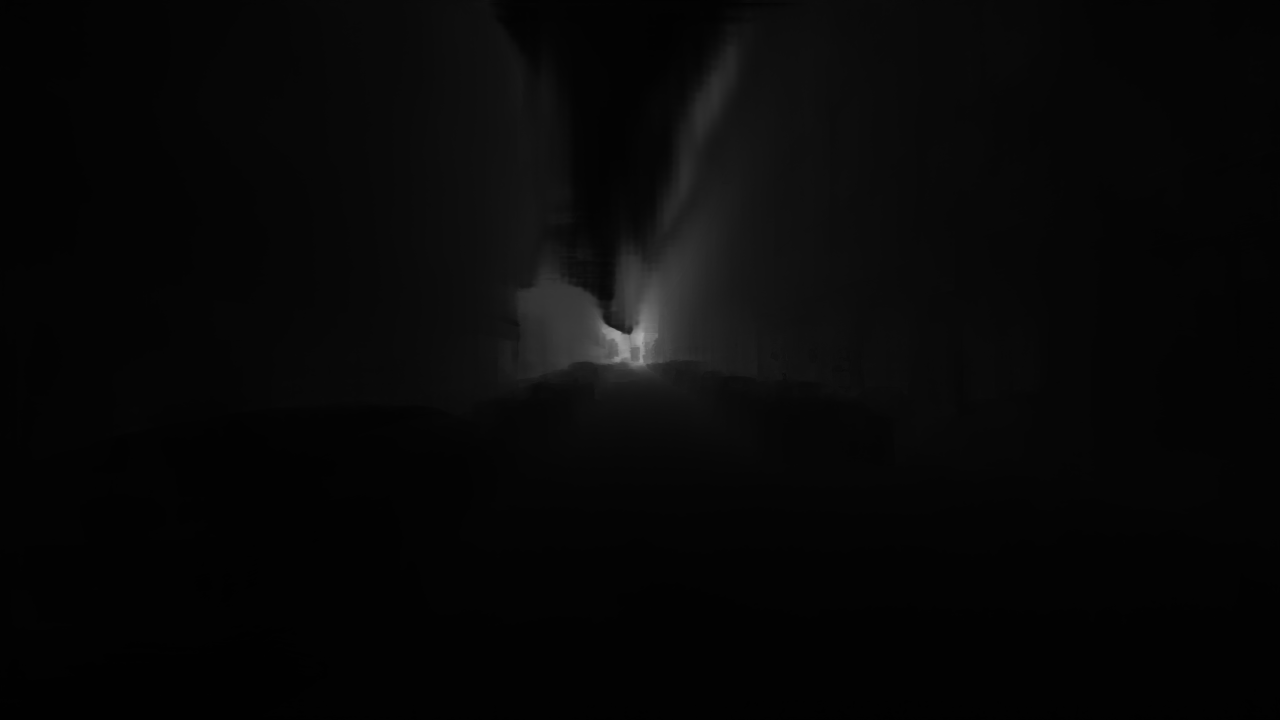
\includegraphics[width=\textwidth, trim=0 200pt 0 200pt, clip]{figures/step38.png}
        \caption{Epoch 38}
        \label{fig:epoch38}
    \end{subfigure}
    \hfill
    \begin{subfigure}{\textwidth}
        \centering
        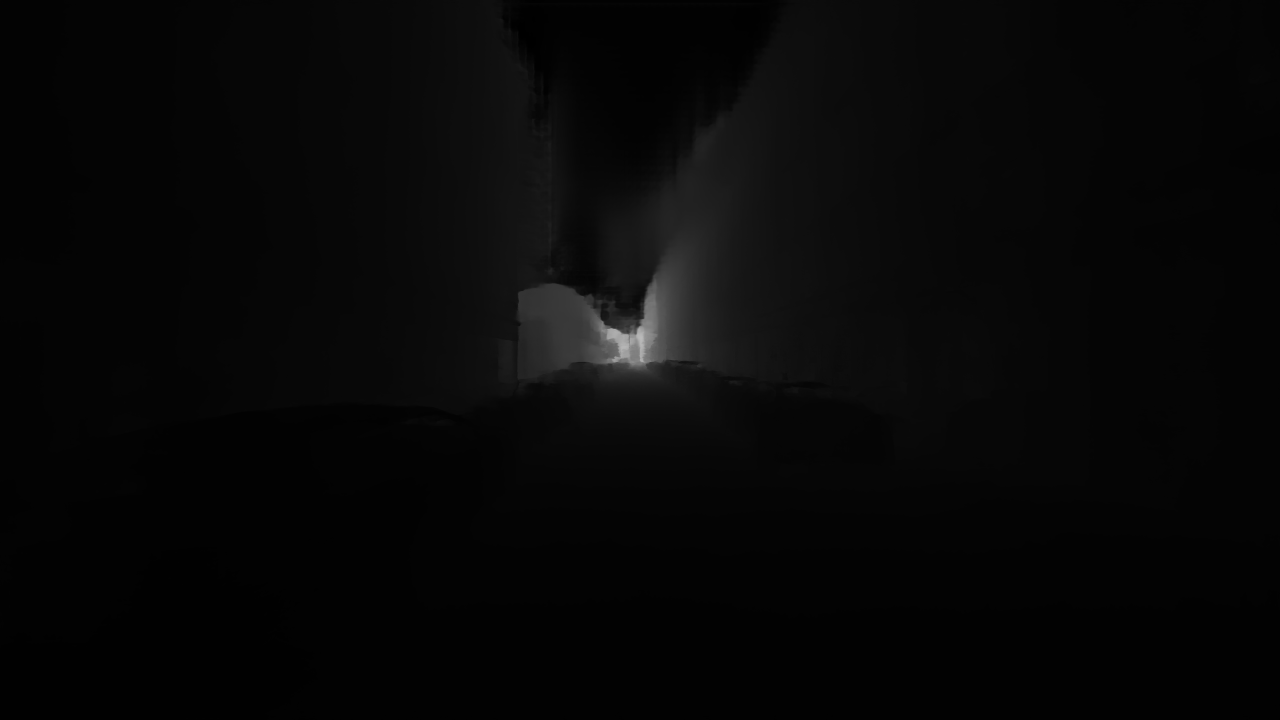
\includegraphics[width=\textwidth, trim=0 200pt 0 200pt, clip]{figures/step99.png}
        \caption{Epoch 99}
        \label{fig:epoch99}
    \end{subfigure}
    \caption{Evolution of depth completion output during training}
    \label{fig:training_progress}
\end{figure}

The sample outputs in Figure \ref{fig:training_progress} demonstrate the model's learning progression through epochs 1, 38, and 99, showing increasingly refined depth estimation and improved preservation of structural details. The final output at epoch 99 exhibits smooth depth transitions and accurate depth completion, indicating successful training despite the oscillations in the validation curve.
\begin{figure}
    \centering
    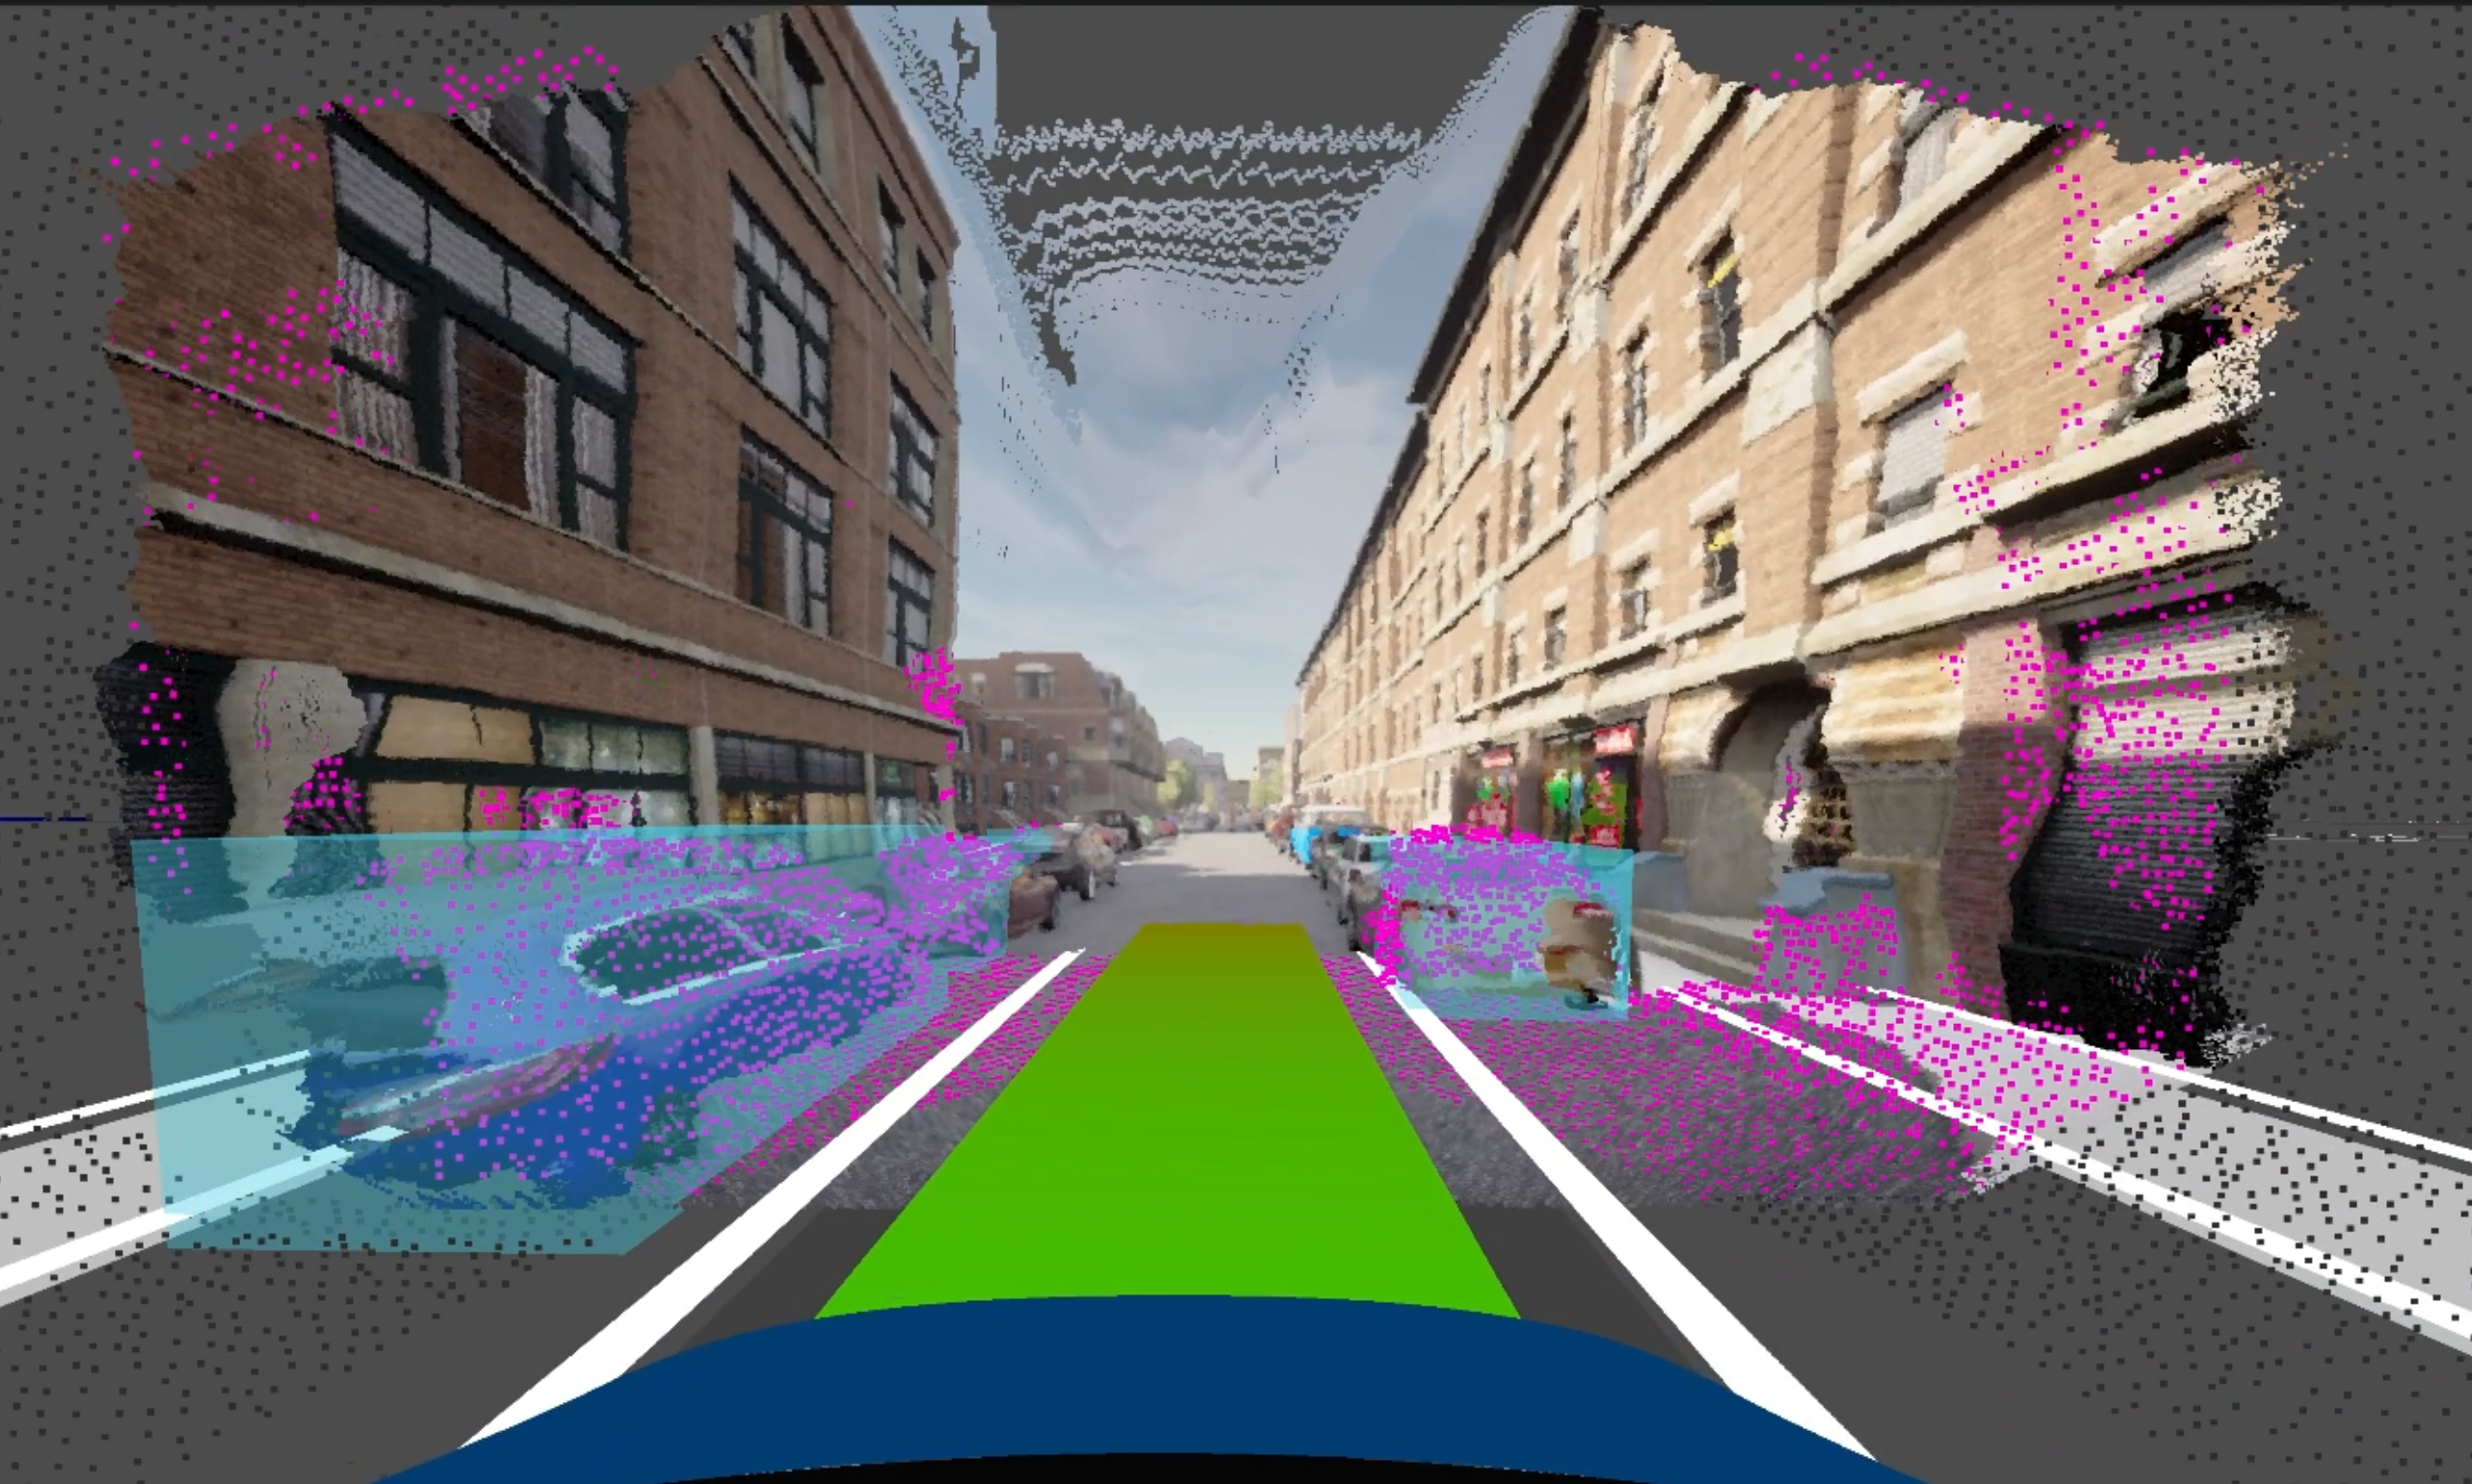
\includegraphics[width=\textwidth, trim=0 150pt 0 50pt, clip]{figures/depth_comp_2.png}
    \caption{The point cloud generated by the output from the depth completion model, colored by camera projection and laid over by other components}
    \label{fig:depth_completion_result}
\end{figure}

\section{Performance Optimization}\label{section:performanceoptimization}

For a teleoperation system to be effective, real-time performance is crucial. Research indicates that system latency should be kept below 300ms for controlled driving, and frame rates should be maintained above 5 Hz to avoid significant performance degradation \cite{neumeier2023feasibility}. Our optimization efforts focus on two main aspects: operator interface performance and network performance.

\subsubsection{Operator Interface Performance}
Our system runs on high-performance hardware, utilizing an NVIDIA RTX 4090 GPU and the latest generation Intel Core i9 processor. Despite this powerful configuration, there are several computational bottlenecks required optimization.

The depth completion model represents our most significant performance bottleneck, requiring 60-70ms per frame for estimation. At this processing speed, the system would be limited to less than 15 fps if processed synchronously. To overcome this limitation, we implemented an asynchronous processing approach where the depth estimation runs on a parallel thread. This allows visual updates to occur at full frame rate while depth information updates at a lower frequency. The difference in update rates is barely noticeable to operators due to the smooth integration of the parallel processing.

The next significant CPU bottleneck involves processing and rendering point cloud data. We addressed this using the PCL library, implementing efficient filtering and concatenation of \ac{LiDAR} inputs. Points that are too close to each other are filtered out to maintain rendering performance while preserving visual quality.
Since we expect high number of points to process, the each iteration effects the performance significantly. On the Point cloud renderer for \emph{Integrated View} we have the advantage of needing less operations

\subsubsection{Network Performance}
Network performance is critical for teleoperation systems, as they must operate within mobile network constraints. Our optimization strategy focuses on minimizing data throughput while maintaining essential information transmission.
We carefully select which data to transmit from vehicle to interface:
\begin{itemize}
\item RGB camera feed (1280x720 resolution)
\item Subset of point cloud data for frontal view
\item Regulatory elements and perception outputs
\end{itemize}
Instead of transmitting full depth images, we send point cloud data in a compressed format. This approach is more efficient as the sparse point cloud contains significant empty space, and point cloud reconstruction occurs on the operator side. Additionally, only relevant points for the frontal view are transmitted, further reducing bandwidth requirements.
Through these optimizations, we maintain real-time performance while working within network bandwidth constraints, ensuring effective teleoperation capability.

% !TeX root = ../main.tex
% Add the above to each chapter to make compiling the PDF easier in some editors.

\chapter{User Study}\label{chapter:userstudy}
The effectiveness of teleoperation interfaces must be evaluated through rigorous user studies to ensure they meet the requirements for situational awareness, cognitive load management, and overall usability. This chapter details our comprehensive user study comparing the Separate View and Integrated View approaches for perception modification tasks.

Our study design focuses on three key aspects identified in the literature review: situational awareness measured through SAGAT, cognitive workload assessed using NASA-TLX, and feature completeness evaluated through expert feedback. To ensure ecological validity and relevance to our target users, we developed a custom simulation environment based on Munich's road infrastructure, moving away from the US-centric scenarios typical in CARLA simulations.

The study incorporates multiple scenarios designed to test different aspects of perception modification tasks, with particular attention to situations where \acp{AV} commonly require human intervention. These scenarios were carefully crafted to evaluate both interfaces under comparable conditions while maintaining realistic challenges faced in urban environments.

This chapter details the methodology of the user study, including scenario selection, questionnaire development, and study execution. We outline the preparation process, including map creation, scenario recording, and video creation. While the analysis of collected data falls outside the scope of this thesis, the study design and execution provide a robust foundation for future research in teleoperation interface evaluation.
\section{Study Design}

The study evaluates three distinct teleoperation interface configurations:

The Separate View (Section \ref{section:separateview}) presents 2D camera feeds and 3D perception data on separate displays, following traditional teleoperation interface designs. This configuration allows operators to view raw sensor data and processed perception information independently.

The Integrated View (Section \ref{section:integratedview}) combines all raw sensor data and perception data in a single window, utilizing our depth completion model to create a comprehensive visualization. This novel approach aims to reduce the cognitive load of switching between different views while maintaining situational awareness.

The Integrated View with Ground Truth is a variant we added just for the study that maintains the same single-window layout but incorporates ground truth depth data instead of the completion model's output. This configuration serves as a baseline for comparison, helping evaluate the effectiveness of our depth completion model against ideal conditions.
Thus we have the research question answered for both the comparison of the Separate View and Integrated View and the evaluation of the depth completion model.

Our evaluation methodology incorporates multiple standardized assessment techniques to comprehensively evaluate these interfaces:

\paragraph{Assesment Framework}
\begin{itemize}
    \item Situational awareness measurement using \ac{SAGAT} \cite{endsley1988sagat} methodology
    \item Cognitive workload evaluation through \ac{NASA-TLX} \cite{hart2006nasa} assessment
    \item Interface usability and feature effectiveness assessment
    \item Comparative analysis of interface variants
\end{itemize}

This comprehensive evaluation framework enables objective comparison of the interfaces while gathering detailed insights into user experience and performance. While the analysis of collected data falls outside the scope of this thesis, the study design ensures that future research can effectively evaluate the relative merits of each interface configuration.

\subsection{Scenarios}
The scenarios for the user study were designed to evaluate the effectiveness of the Separate View and Integrated View interfaces in supporting perception modification tasks. The goal was to create a diverse set of scenarios that reflect real-world challenges in autonomous driving, focusing on three main categories: modification of objects, modification of drivable space, and unsolvable scenarios. Each category includes multiple variants to ensure comprehensive testing across different situations.
\subsubsection{Modification of Objects}
These scenarios involve correcting misperceptions related to objects detected by the \ac{AV}'s perception system. They test the operator's ability to identify and modify object-related errors in detection, classification, prediction, and position/size:
\begin{table}[h!]
    \centering
    \begin{tabular}{|p{6cm}|p{7.8cm}|}
    \hline
    \textbf{Scenario} & \textbf{Description} \\
    \hline
    Water pond detected as an object & Tests the operator's ability to identify false-positive detections. \\ \hline
    Leaves on the road misclassified & Evaluates how operators handle misclassification of small objects. \\ \hline
    Smoke coming from the sewer on the road misclassified (Figure \ref{fig:scenario_smoke})& Similar to the leaves scenario but with a different object type. \\ \hline
    Pedestrians at a crosswalk not intending to cross (Figure \ref{fig:scenario_crosswalk}) & Challenges operators to correct prediction errors. \\ \hline
    Second-row parker detected as a dynamic vehicle (Figure \ref{fig:scenario_srp}) & Tests handling of incorrect dynamic predictions. \\ \hline
    Tree branches leaning onto the road detected as blocking objects & Wrong classification of the tree branches. \\ \hline
    Harsh light blocking the view for traffic lights & Tests operator's ability to understand the effect of different weather conditions on the system. \\ \hline
    \end{tabular}
    \caption{Scenarios for object modification tasks}
    \label{table:scenariosobjectmodification}
    \end{table}
\subsubsection{Modification of Drivable Space}
These scenarios test how well operators can modify errors in the perceived drivable area:
\begin{table}[h!]
    \centering
    \begin{tabular}{|p{6cm}|p{7.8cm}|}
    \hline
    \textbf{Scenario} & \textbf{Description} \\
    \hline
    Construction site (Figure \ref{fig:scenario_construction}) (two variants) & Evaluates operators' ability to adjust drivable space around construction zones. \\ \hline
    Traffic island detected as an undefined object & Tests corrections for drivable area misinterpretations. \\ \hline
    \end{tabular}
    \caption{Scenarios for drivable area modification tasks}
    \label{table:scenariosdrivablemodification}
    \end{table}

\subsubsection{Unsolvable Scenarios}
These scenarios represent edge cases where no modifications can resolve the issue. They test how operators handle situations beyond their control:

\begin{table}[h!]
    \centering
    \begin{tabular}{|p{6cm}|p{7.8cm}|}
    \hline
    \textbf{Scenario} & \textbf{Description} \\
    \hline
    Completely occluded traffic light blocked by a truck & Evaluates decision-making when critical information is unavailable. \\ \hline
    Blocked one-way street & Tests operator responses to unresolvable roadblocks. \\ \hline
    \end{tabular}
    \caption{Scenarios for unsolvable tasks}
    \label{table:scenariosunsolvable}
    \end{table}

The scenarios were selected from a subset defined in El Alami's thesis \cite{yassinethesis}, focusing on those most relevant to perception modification tasks. Each scenario was designed to ensure consistency across tests while remaining challenging enough to evaluate operator performance effectively.

\begin{figure}
    \centering
    \begin{subfigure}[b]{0.45\textwidth}
        \centering
        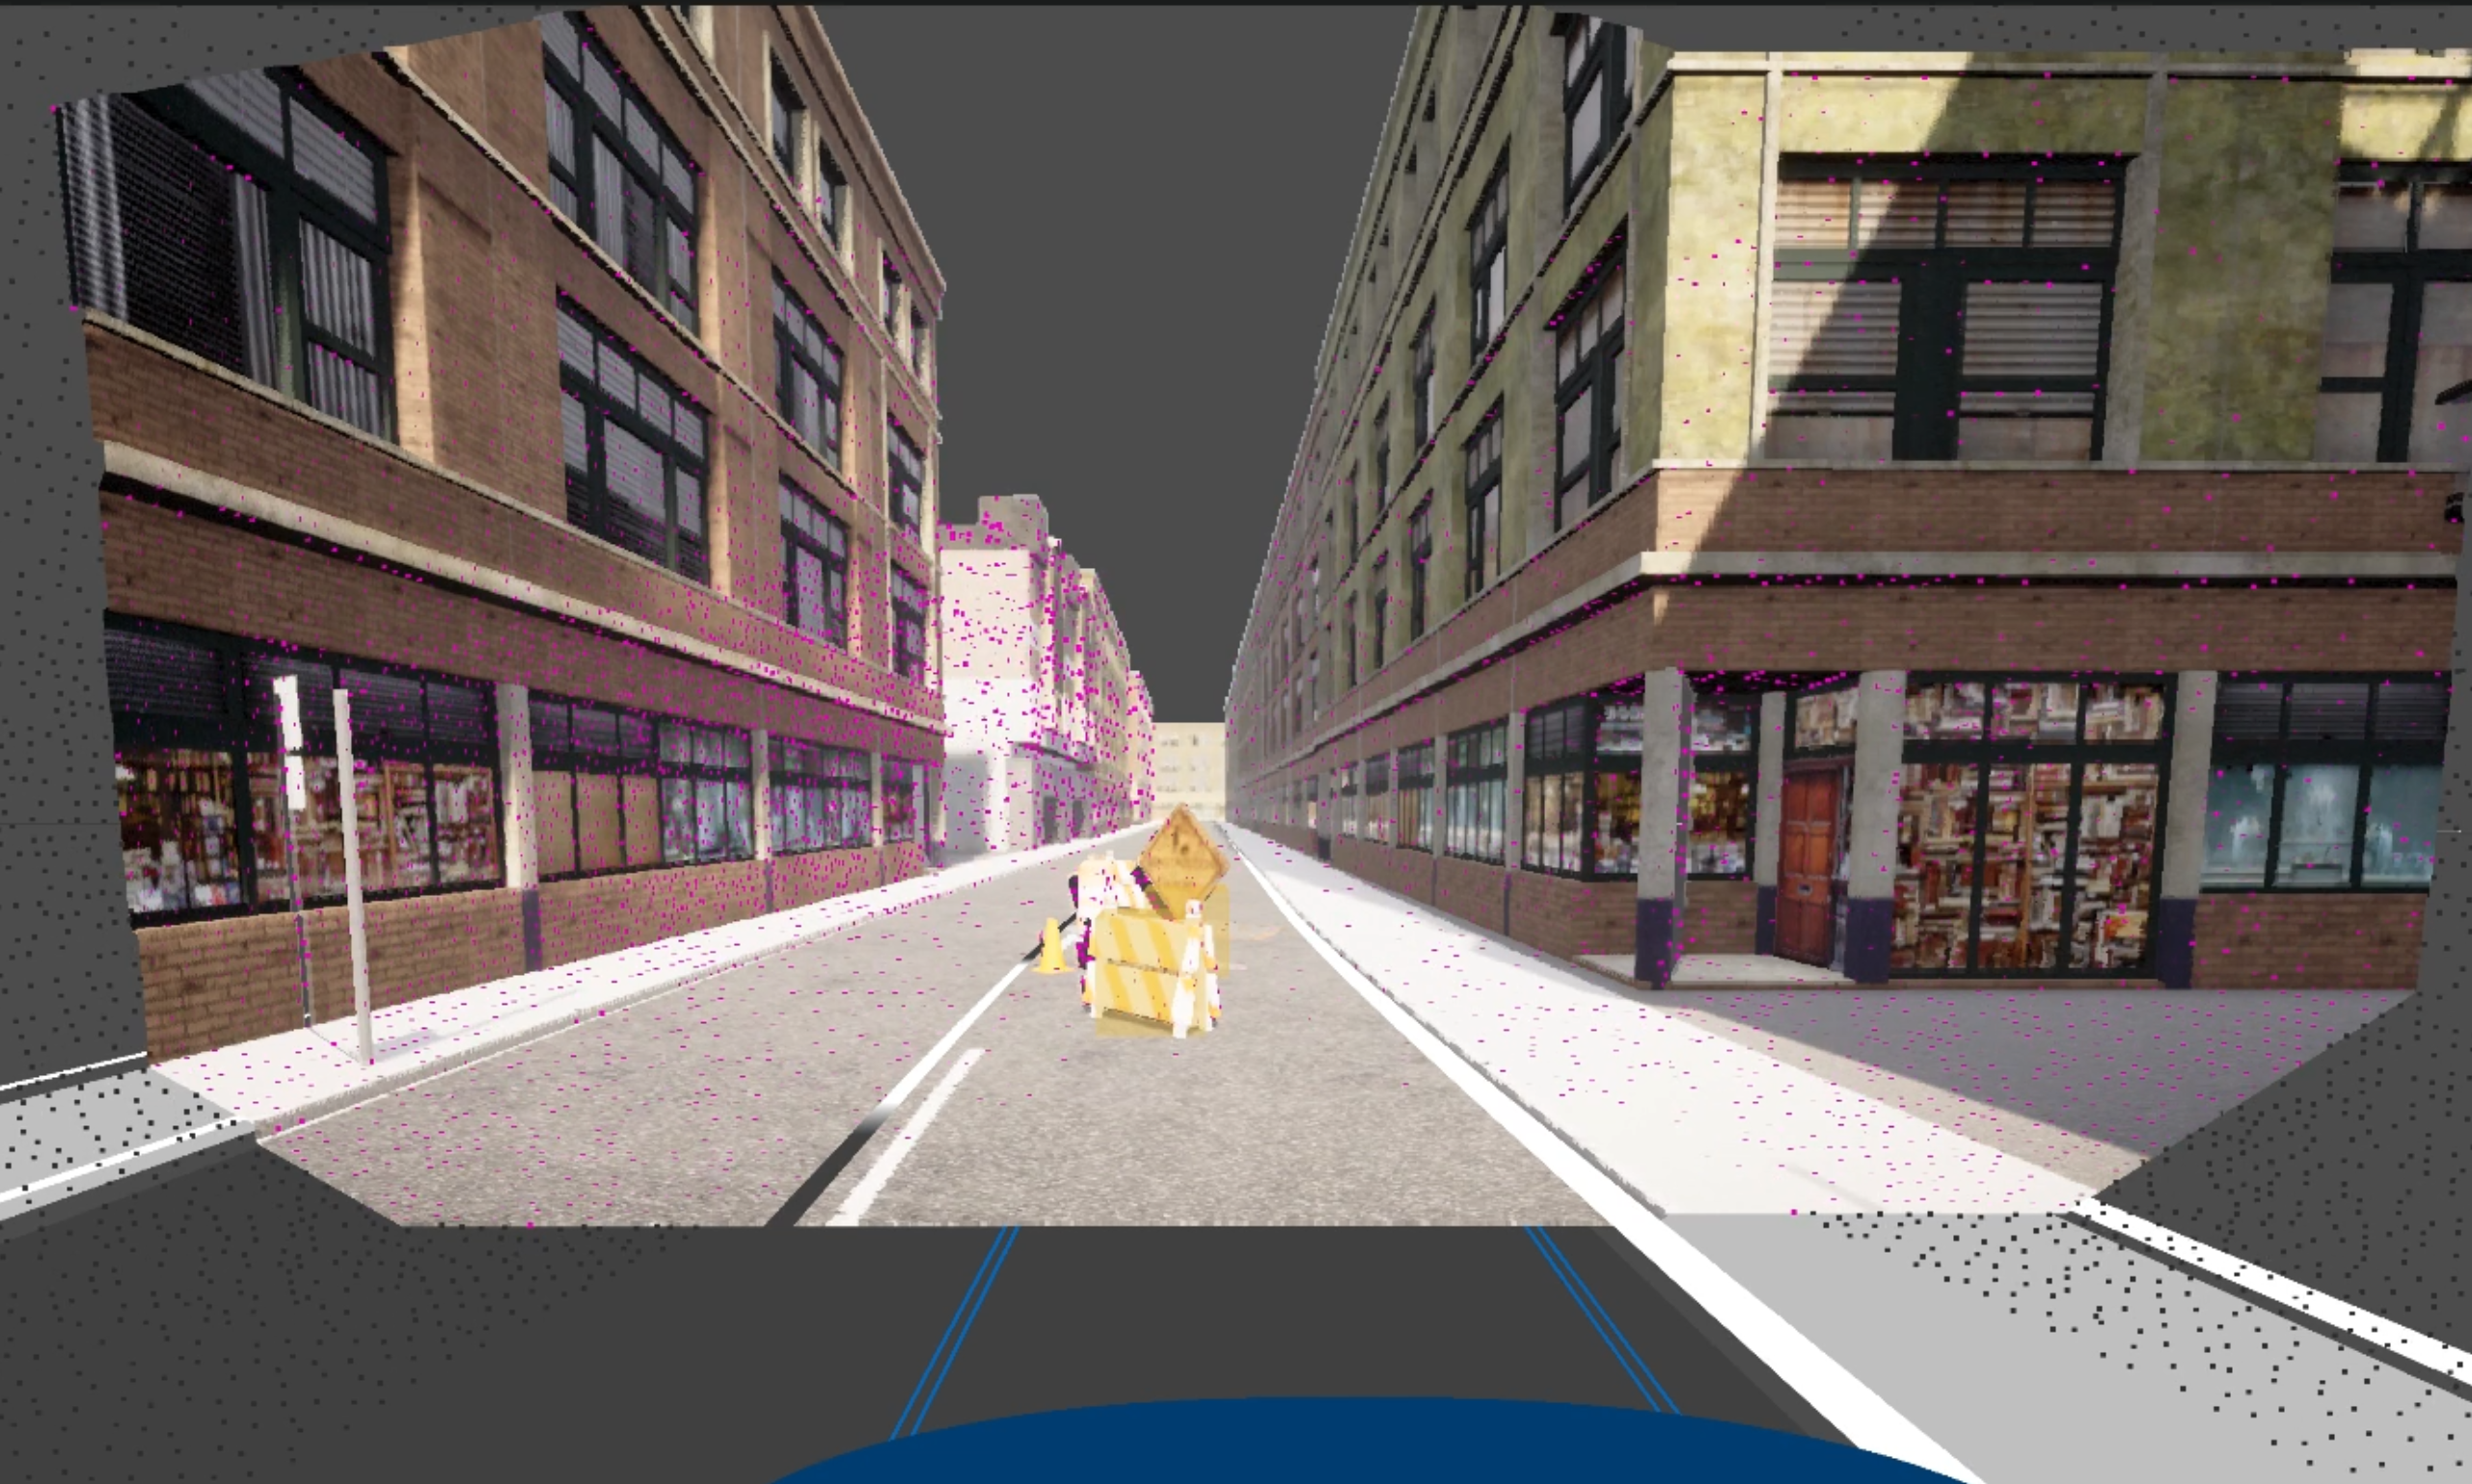
\includegraphics[width=\textwidth]{figures/scenario_cons.png}
        \caption{Construction site scenario}
        \label{fig:scenario_construction}
    \end{subfigure}
    \hfill
    \begin{subfigure}[b]{0.45\textwidth}
        \centering
        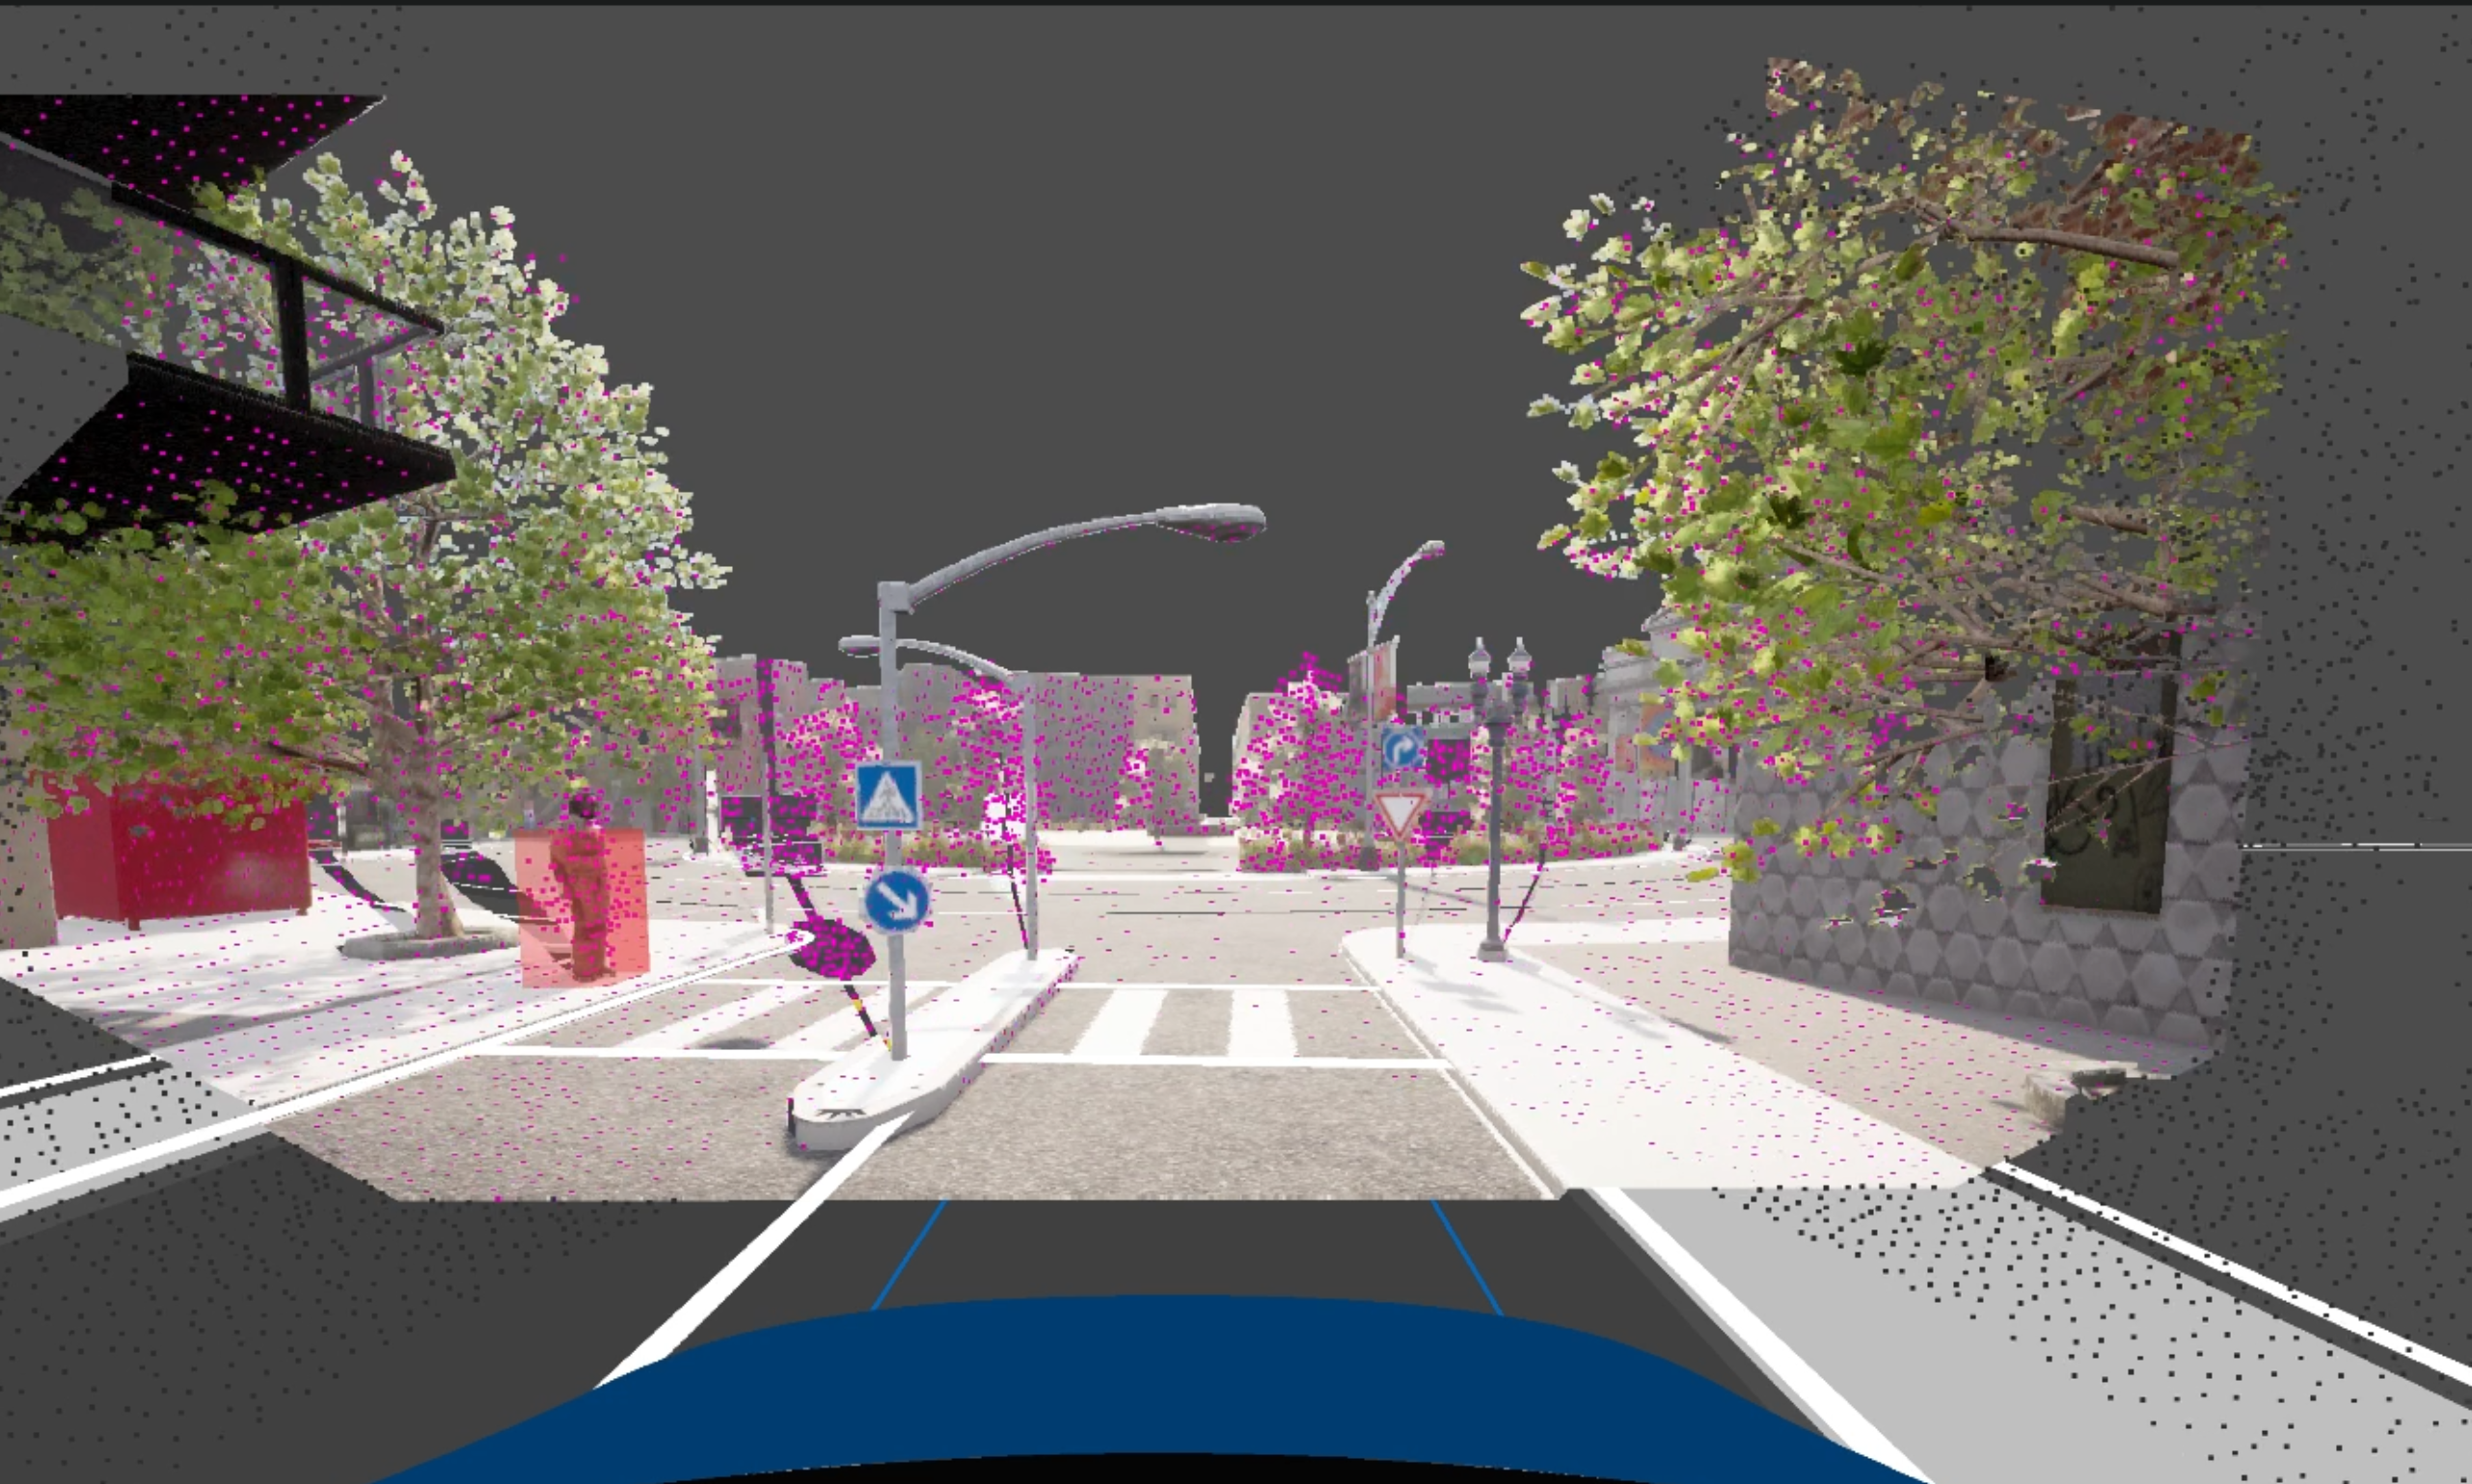
\includegraphics[width=\textwidth]{figures/scenario_cross.png}
        \caption{Pedestrians at a crosswalk scenario}
        \label{fig:scenario_crosswalk}
    \end{subfigure}
    \newline
    \begin{subfigure}[b]{0.45\textwidth}
        \centering
        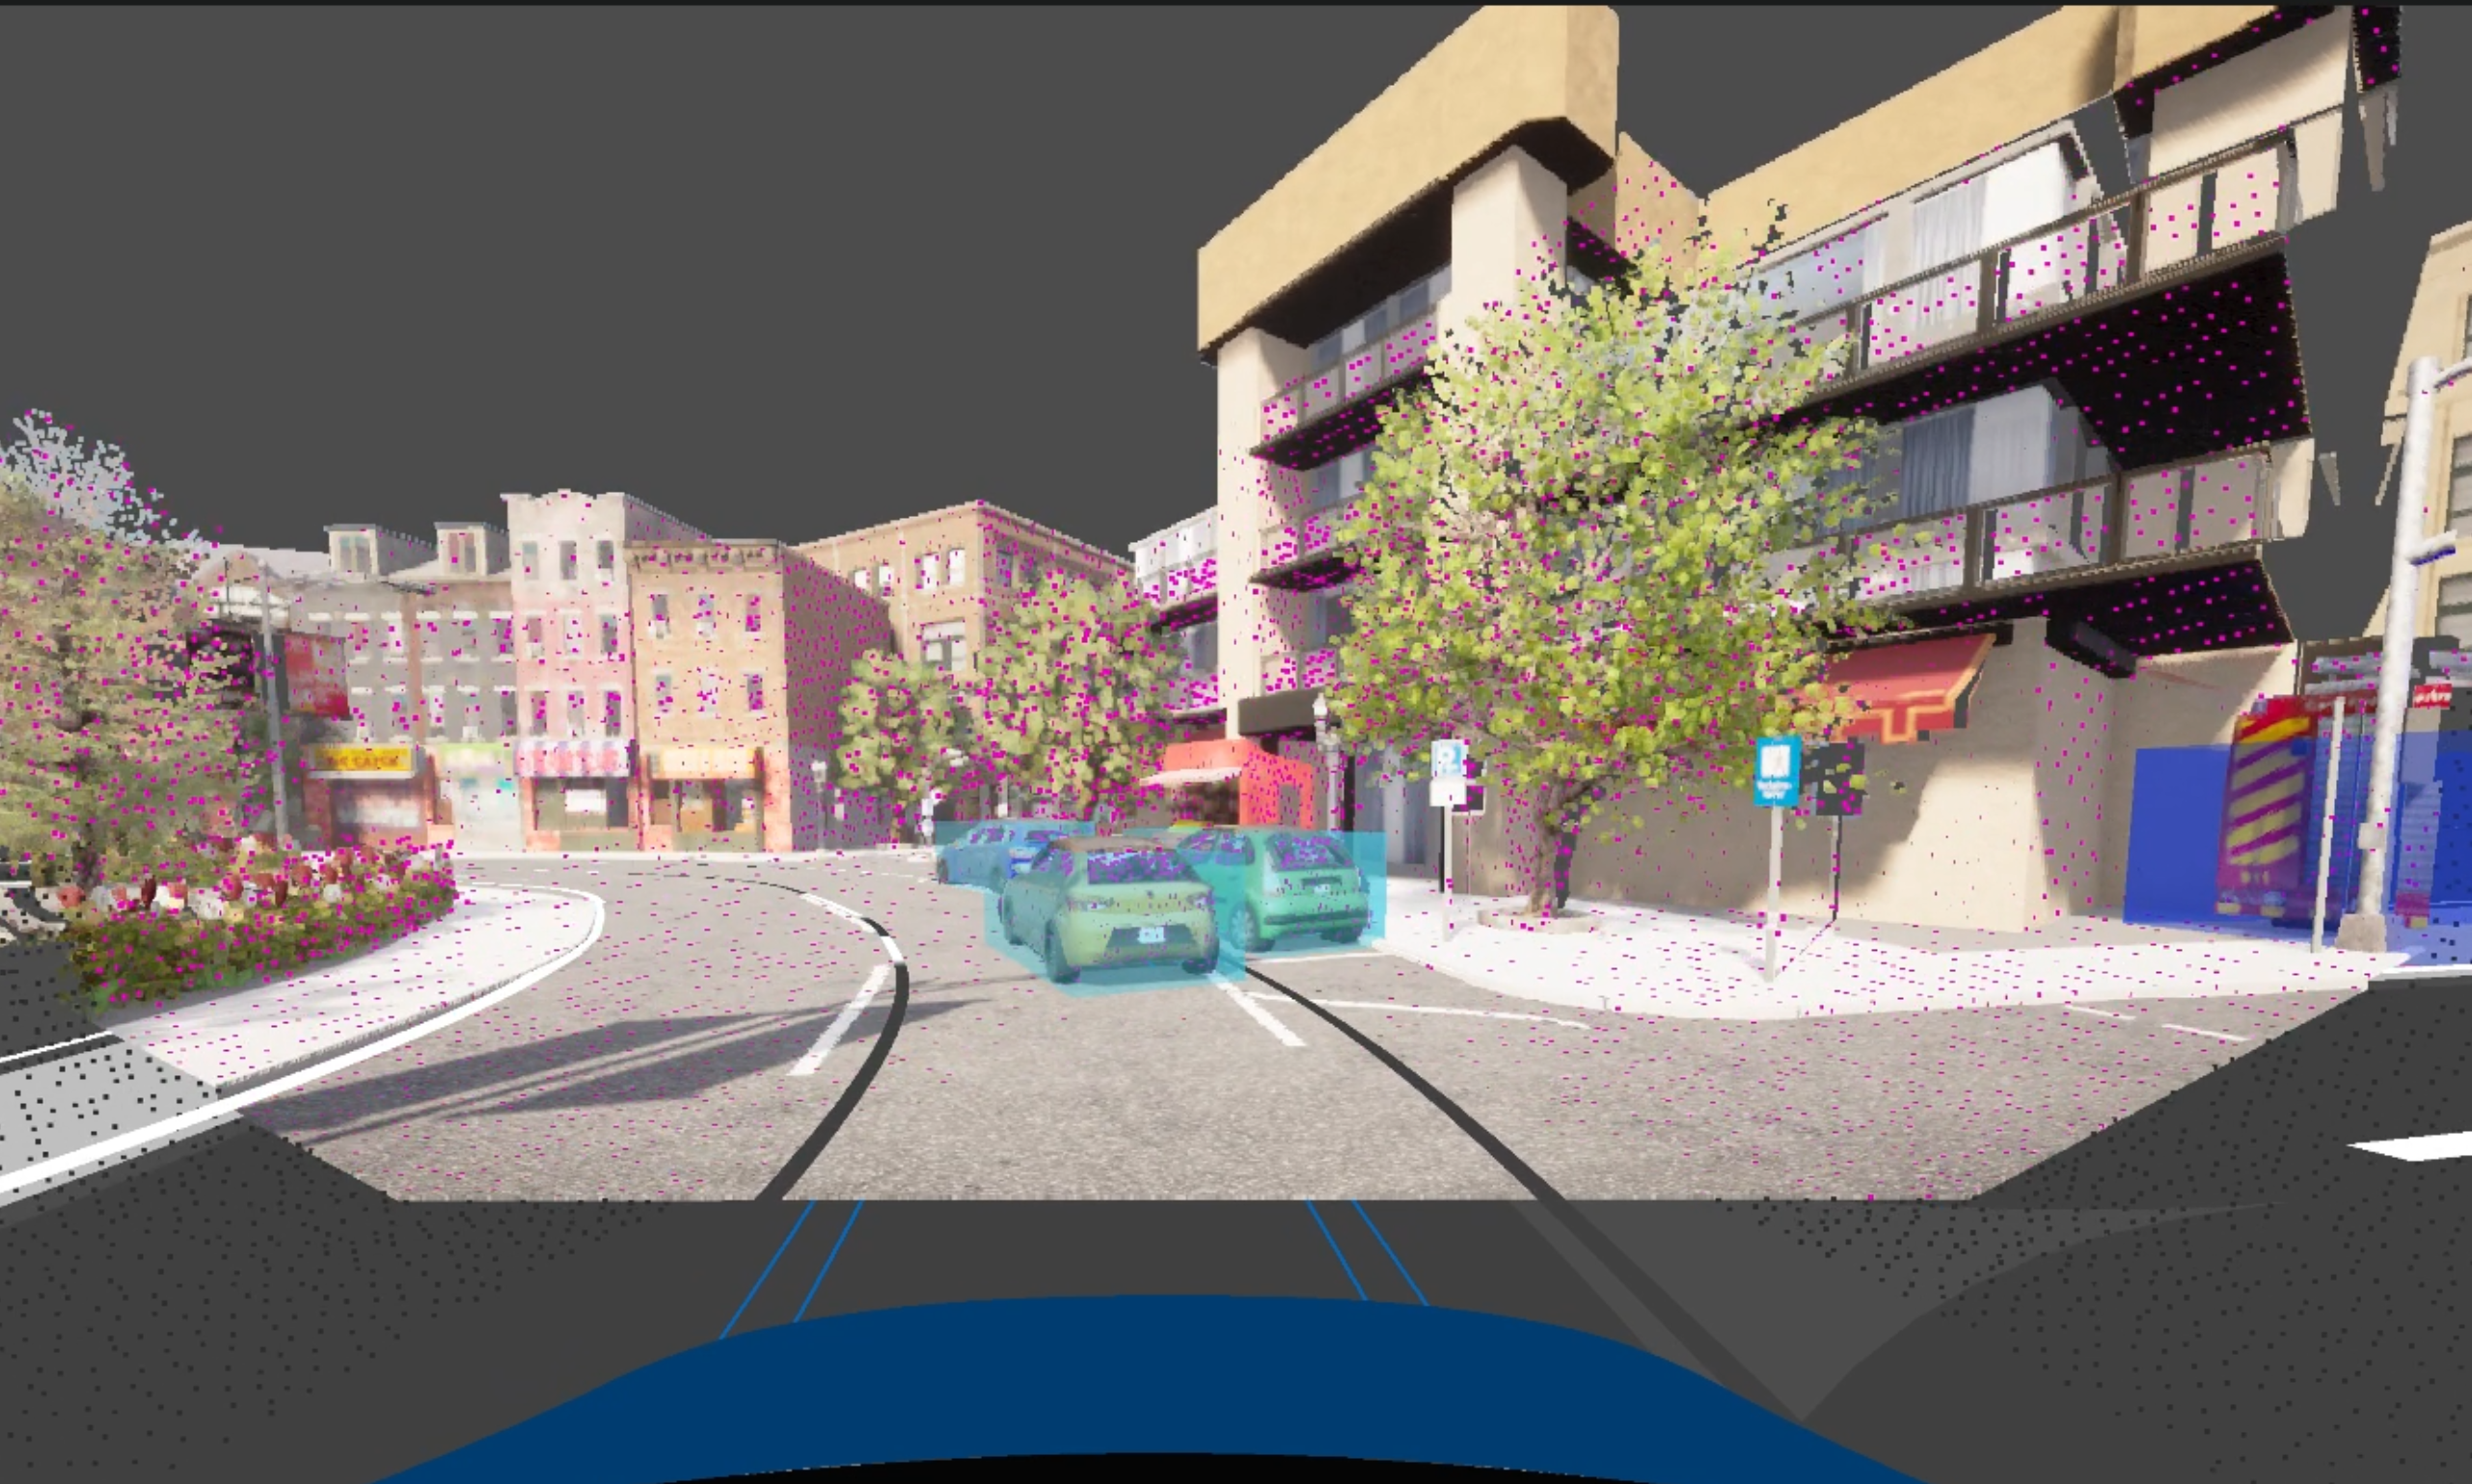
\includegraphics[width=\textwidth]{figures/scenario_srp.png}
        \caption{Second row parker scenario}
        \label{fig:scenario_srp}
    \end{subfigure}
    \hfill
    \begin{subfigure}[b]{0.45\textwidth}
        \centering
        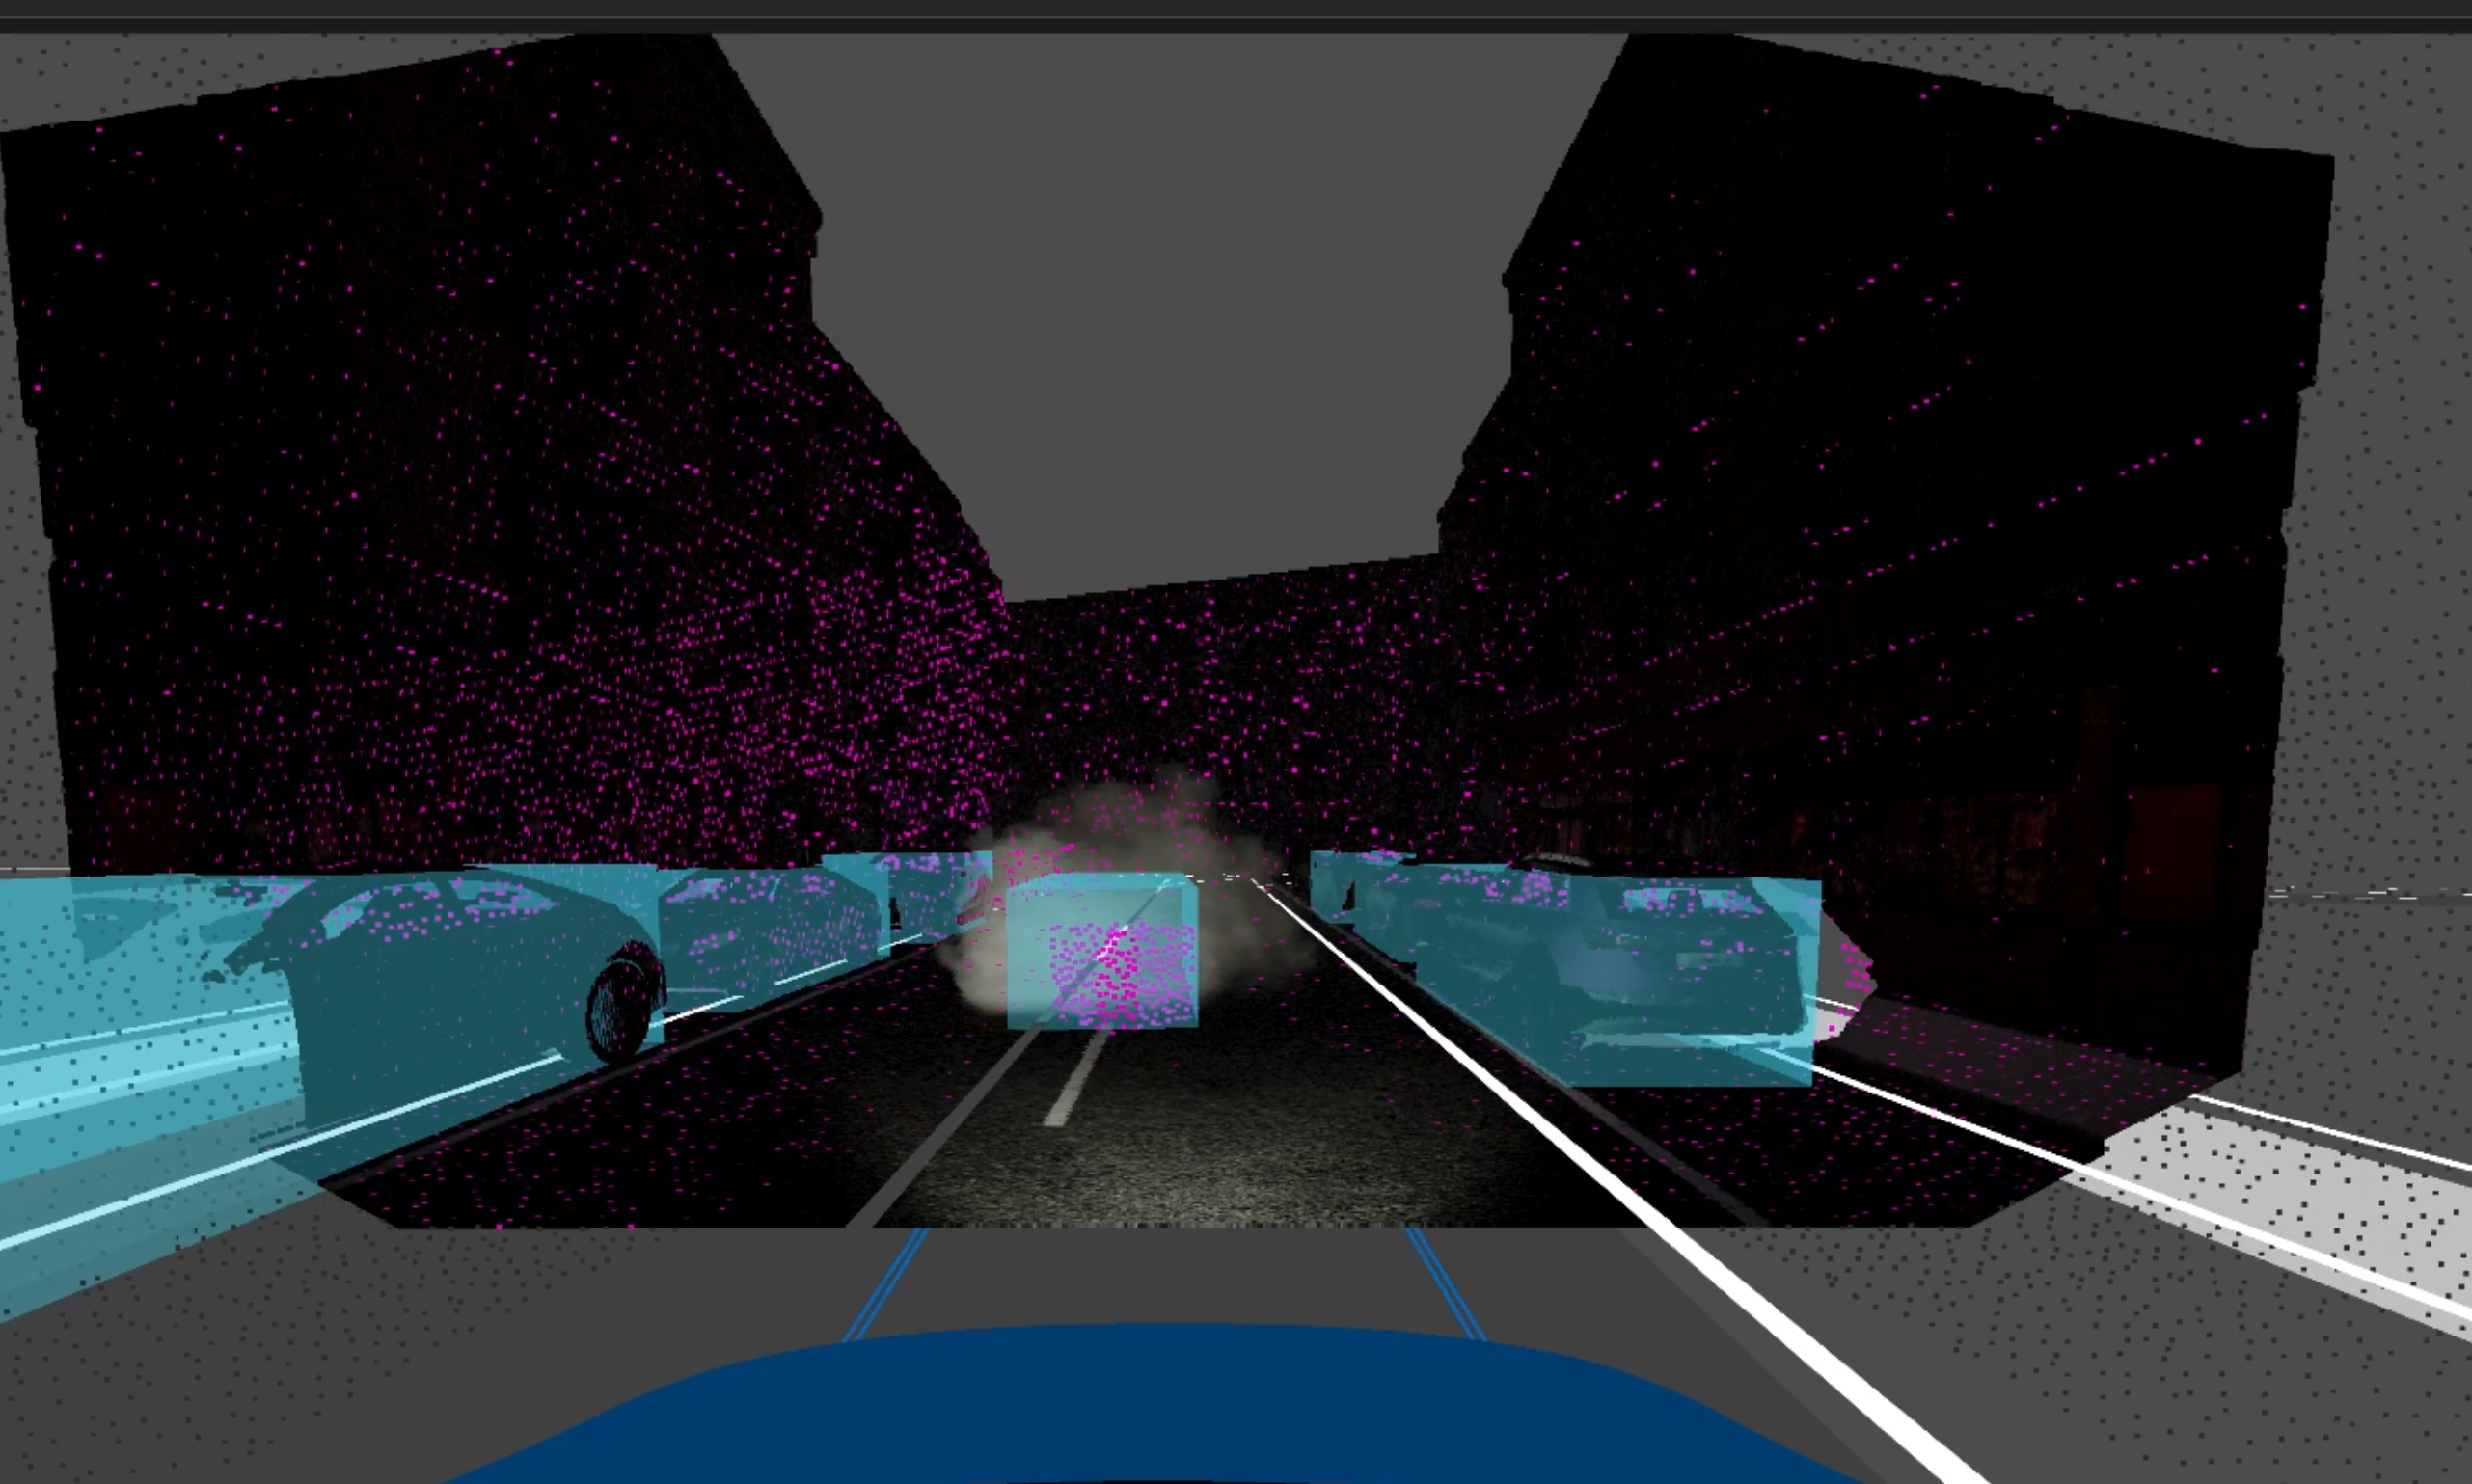
\includegraphics[width=\textwidth]{figures/scenario_smoke.png}
        \caption{Smoke from sewer scenario}
        \label{fig:scenario_smoke}
    \end{subfigure}
    \caption{Scenarios for object modification tasks}
    \label{fig:full}
\end{figure}


\subsection{Questionnaire}
The questionnaire for evaluating the visualization interfaces combines standardized assessment tools with custom questions specific to perception modification tasks. Developed by Tobias Kerbl, the questionnaire structure follows a comprehensive approach to gather both objective and subjective feedback from participants. For this thesis, we use a subset of the questions focusing on situational awareness, mental workload, and specific subjective evaluations to compare the interface variants.

The demographic section collects information about participants' backgrounds, including age, gender, driving experience, and familiarity with video games and technical systems. This data helps analyze whether certain user characteristics influence performance with different visualization approaches.

For assessing situational awareness, we employ the \ac{SAGAT}. The \ac{SAGAT} questions are customized for each scenario and cover all three levels of situation awareness: perception (Level 1), comprehension (Level 2), and projection (Level 3). This method, developed by Endsley \cite{endsley1988sagat}, allows for an objective measurement of participants' understanding of the current environment, their ability to integrate this information, and their capacity to predict future states. We slightly modified the original \ac{SAGAT} questions to better fit the perception modification tasks in our study. Our design consist of having one question for each level of situation awareness for each scenario.
\begin{table}[h!]
    \centering
    \begin{tabular}{|p{6cm}|p{7.8cm}|}
    \hline
    \textbf{SAGAT Level} & \textbf{Question} \\
    \hline
    Level 1 (Perception) & 4-5 statements per scenario. We expect the user to mark the correct ones. Example Statement: The vehicle trajectory was blocked by an undefined object. \\ \hline
    Level 2 (Comprehension) & Free-text question to question if the participants understand why the \ac{AV} stopped in the scenario \\ \hline
    Level 3 (Projection) & Multiple choice question that gives the possible outcomes after applying an operator modification on the scenario and measures the participants understanding on the vehicle behavior afterwards. \\ \hline
    \end{tabular}
    \caption{Questions to measure \ac{SA}}
    \label{table:scenariosunsolvable}
    \end{table}

Mental workload is evaluated using the \ac{NASA-TLX} \cite{hart1988development}, focusing on dimensions such as mental demand and frustration level. This tool, widely used in human factors research, provides insights into the cognitive demands placed on operators during teleoperation tasks.

After each interface variant, participants provide subjective feedback on usability and feature effectiveness. This includes evaluating specific visualization elements such as point cloud representation, bounding box visualization, traffic element rendering, and prediction visualization. These questions are designed to capture participants' perceptions of the interface's ability to support perception modification tasks.

The questionnaire concludes with comparative questions where participants rank the interface variants and provide qualitative feedback on their preferences and suggested improvements. This section aims to gather insights into which aspects of each interface were most effective and where improvements could be made.
\section{Study Preparation}

The preparation phase of our user study required careful attention to three key components to ensure consistent and reproducible results across all participants. This section details the systematic approach taken to create a controlled yet realistic testing environment.

First, we developed a custom simulation environment based on Munich's Gärtnerplatz square, moving away from generic or US-centric scenarios typical in autonomous driving research. The map creation process, detailed in Section \ref{section:mapcreationforcarla}, involved translating real-world geographical data into a format suitable for the CARLA simulator while maintaining the location's distinctive features.

Following the environment creation, we implemented a structured scenario recording workflow that combines CARLA simulation with Autoware's autonomous driving stack. This process, which presented several technical challenges in maintaining data quality while managing computational constraints, ensures that each test scenario is reproducible and consistent across different interface evaluations.

Finally, we developed a standardized video creation pipeline to ensure consistent scenario playback across the three interface variants. This step was crucial in ensuring that participants could evaluate all three interface variants - the Separate View, Integrated View, and Integrated View with Ground Truth - under identical conditions.

The following subsections detail each of these preparation steps, describing the technical implementation, challenges encountered, and solutions developed to create a robust experimental framework.


\subsection{Map creation for CARLA}\label{section:mapcreationforcarla}
To ensure the ecological validity of our user study and provide a realistic simulation environment, we developed a custom map for CARLA based on the Gärtnerplatz square in Munich, Germany. This section describes the map creation process, which involved replicating the real-world location as closely as possible while adapting it to the capabilities of the CARLA simulator.
\subsubsection*{Pipeline Overview}
\begin{figure}
    \centering
    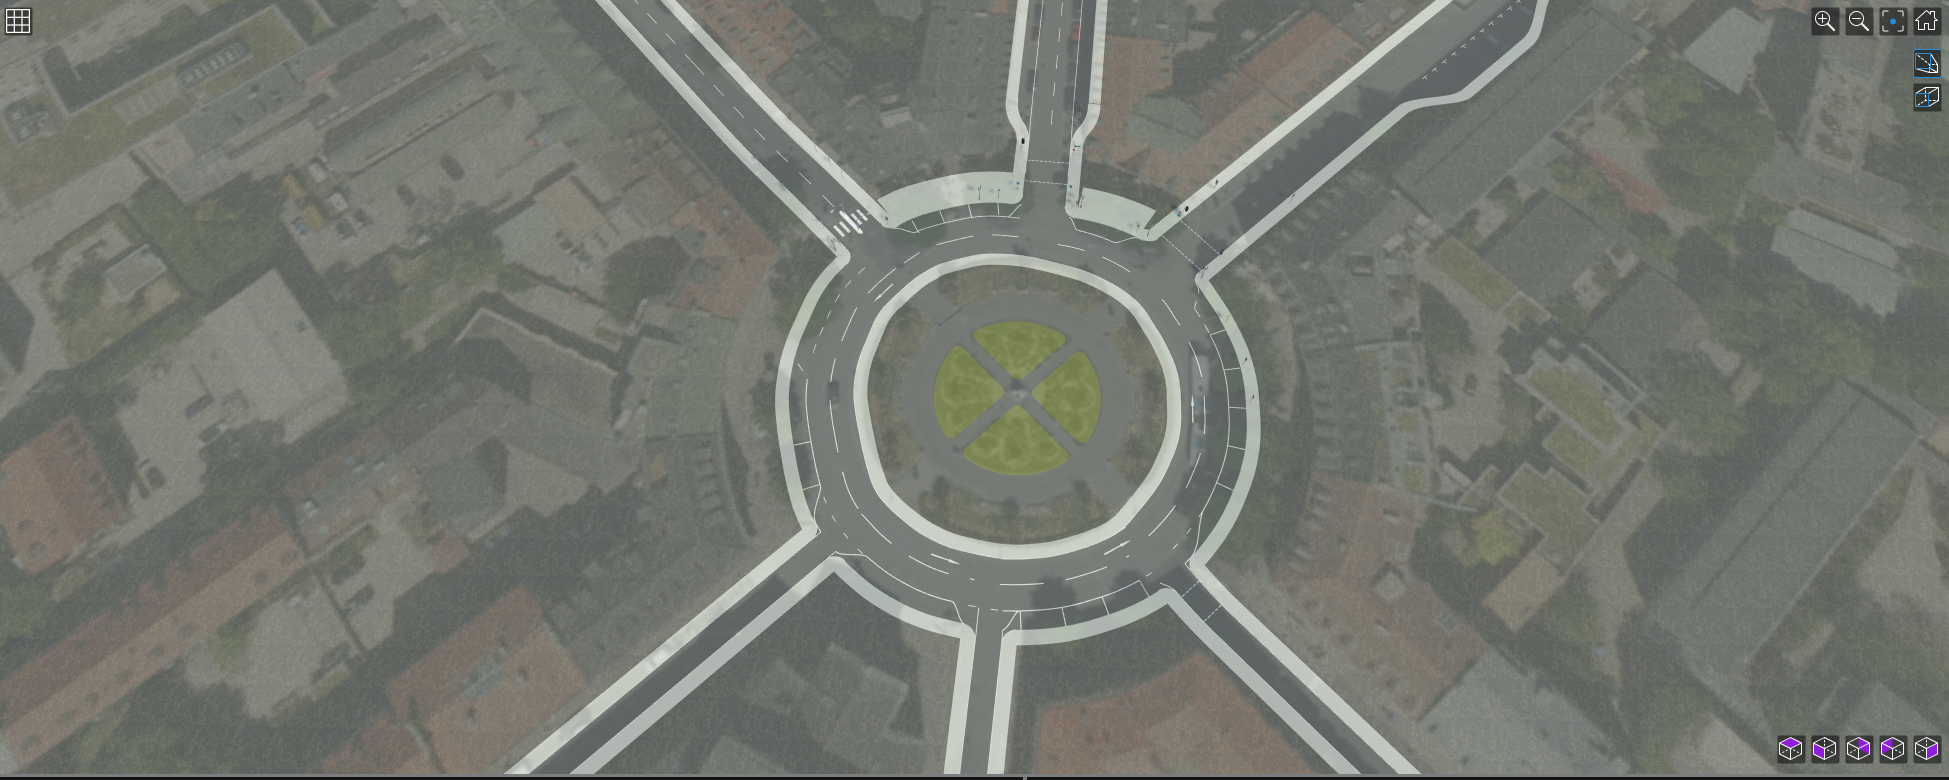
\includegraphics[width=\textwidth]{figures/roadrunner.png}
    \caption{Road network design of Gärtnerplatz in MathWorks RoadRunner}
    \label{fig:roadrunner}
\end{figure}
The map creation process followed a structured pipeline:
\begin{enumerate}
    \item Road Network Creation: Using MathWorks RoadRunner, we designed the road network based on satellite data obtained from the Geoportal Bayern \cite{geoportal_bayern}. The road network included all major features of Gärtnerplatz, such as the six-way roundabout, one-way roads, two-way roads with traffic islands, and traffic lights at intersections. Regulatory elements like crosswalks, traffic signs, and lane markings were added to align with real-world traffic rules. The results can be seen in Result can be seen in \ref{fig:roadrunner}.
    \item Export to OpenDRIVE: The road network and regulatory elements were exported in OpenDRIVE format using RoadRunner's export tools \cite{mathworks_roadrunner}.
    \item Import into Unreal Engine: The OpenDRIVE file and associated assets were imported into Unreal Engine using CARLA's RoadRunner import plugin \cite{carla_map_import}. This step included setting up the road geometry, lane configurations, and traffic rules within CARLA's simulation environment.
    \item Environment Art: Additional environment details, such as buildings, vegetation, and textures, were created in Unreal Engine using CARLA's default asset set. The visual elements were designed to replicate the appearance of Gärtnerplatz as closely as possible.
\end{enumerate}

\begin{figure}[h]
    \centering
    \begin{subfigure}{\textwidth}
        \centering
        \includegraphics[width=\textwidth, trim=0 200pt 0 200pt, clip]{figures/sim_top.png}
        \caption{Top view of the simulation environment}
        \label{fig:sim_top}
    \end{subfigure}
    \begin{subfigure}{\textwidth}
        \centering
        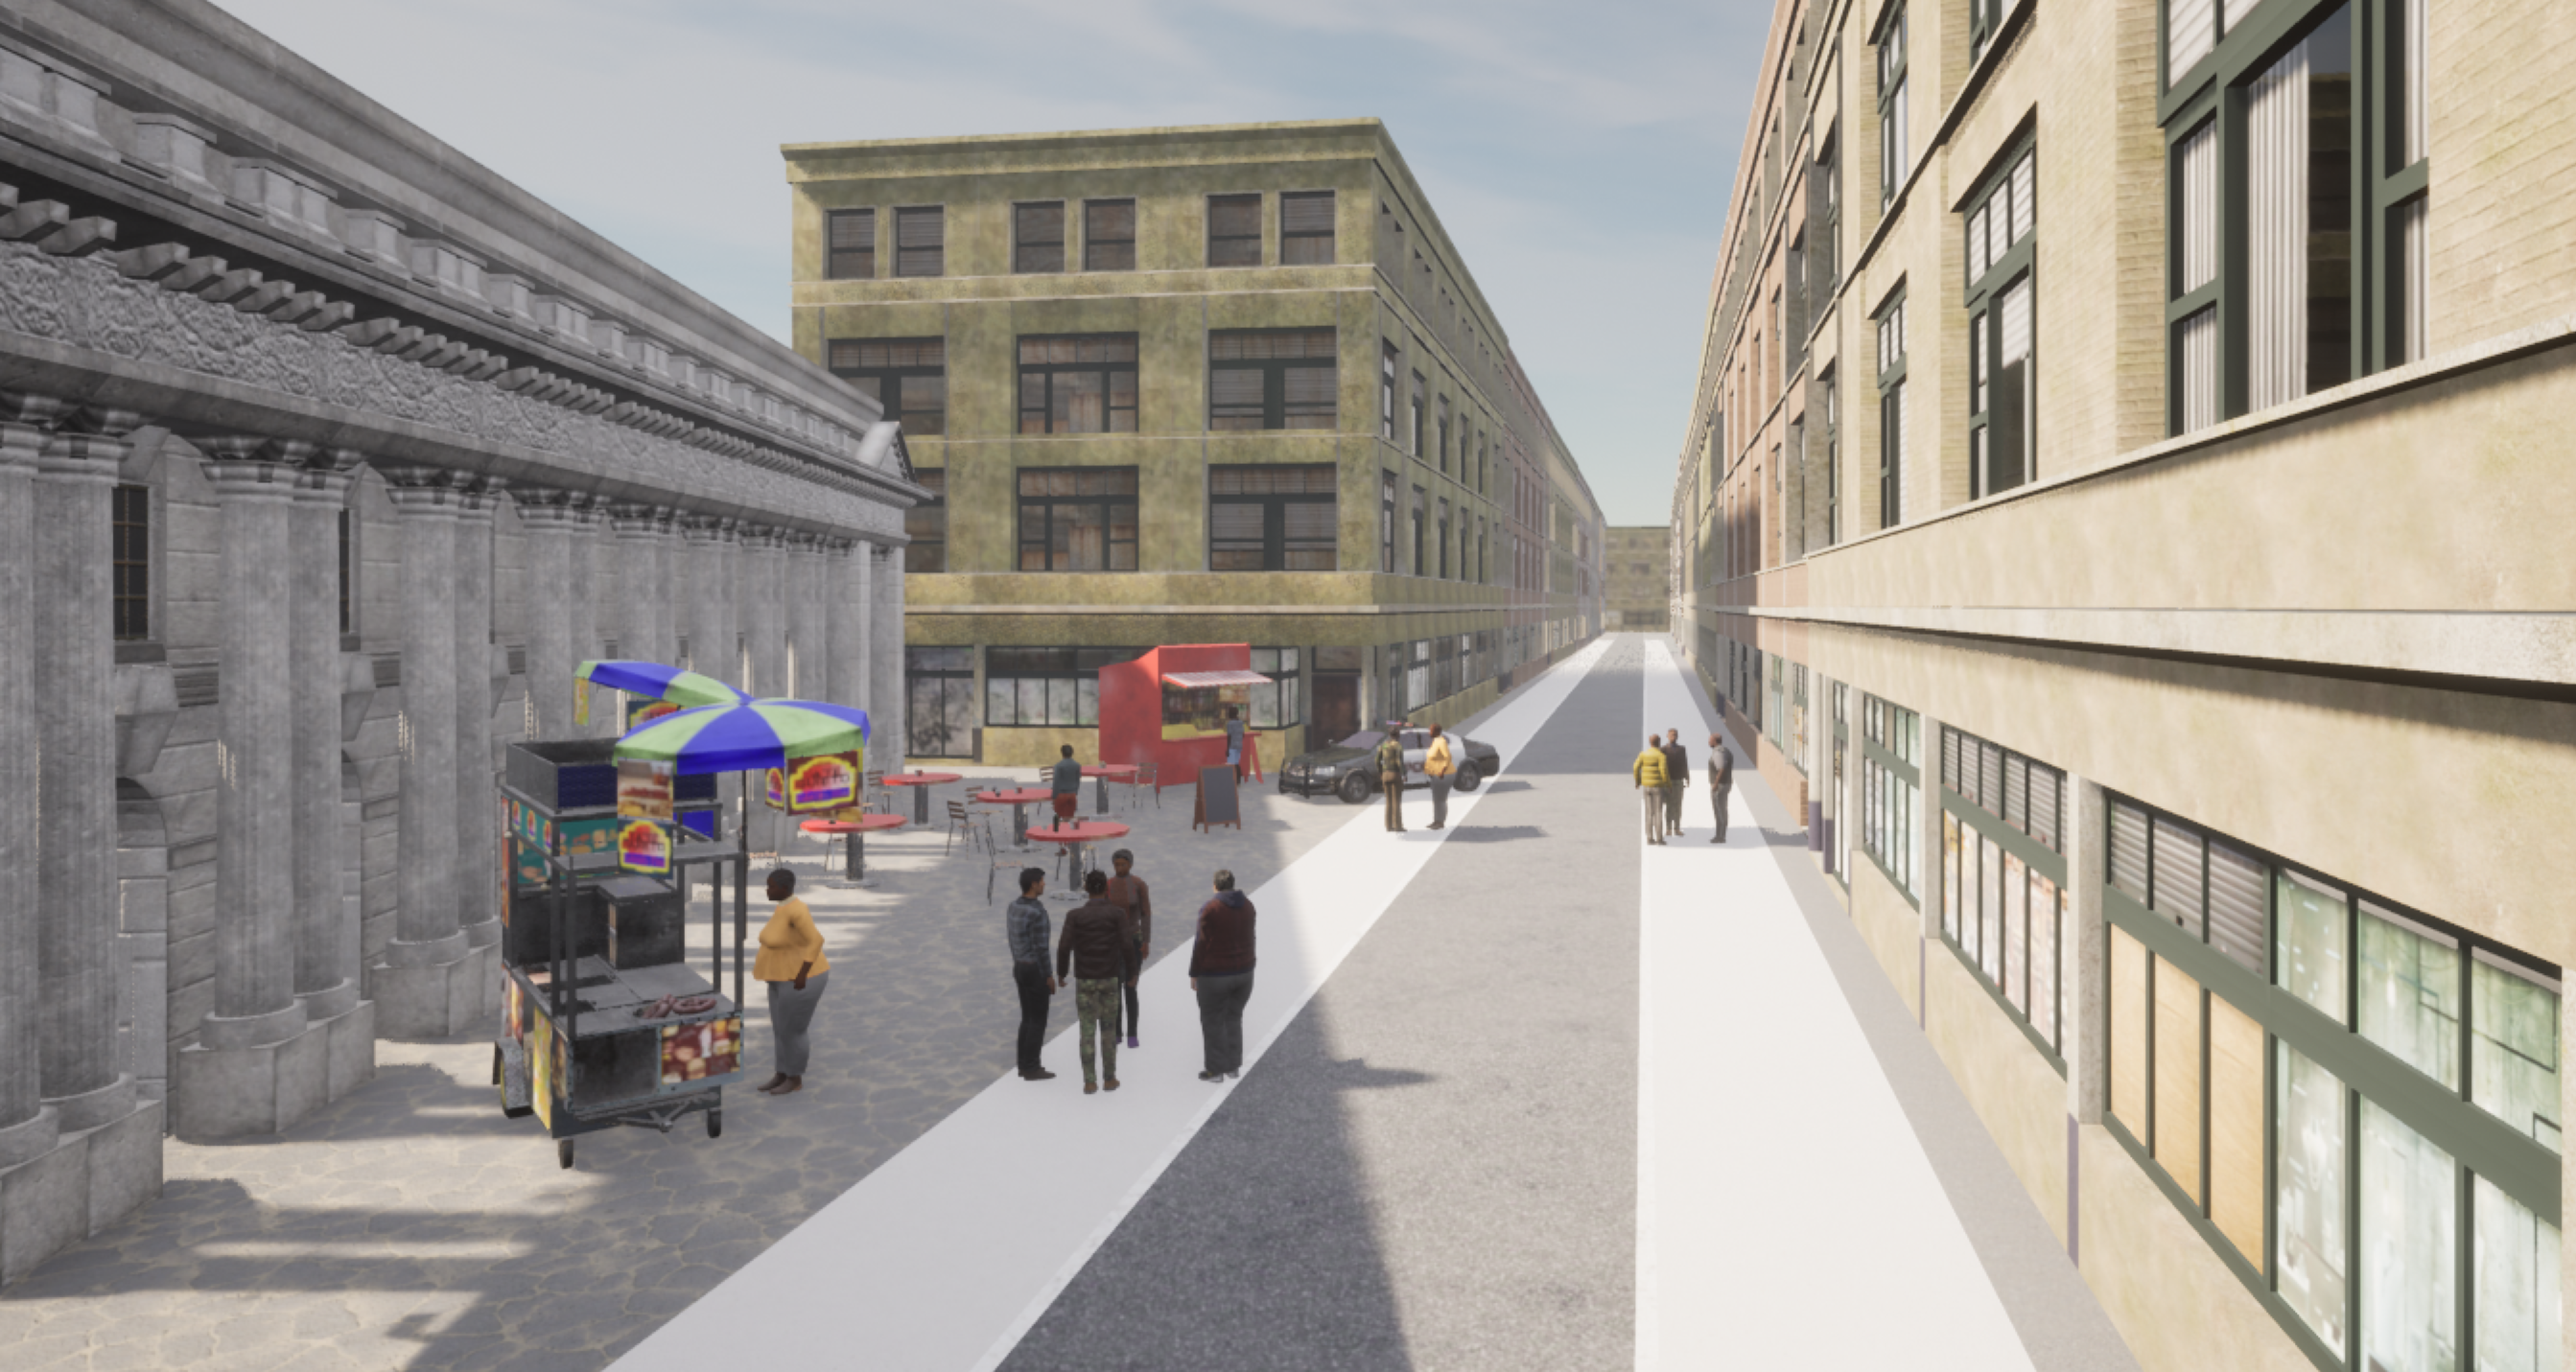
\includegraphics[width=\textwidth, trim=0 200pt 0 200pt, clip]{figures/sim_crowd.png}
        \caption{Environment is detailed to provide a dynamic city look}
        \label{fig:sim_crowd}
    \end{subfigure}
    \begin{subfigure}{\textwidth}
        \centering
        \includegraphics[width=\textwidth, trim=0 200pt 0 200pt, clip]{figures/sim_signs.png}
        \caption{Local traffic signs are used in their real-world locations}
        \label{fig:sim_signs}
    \end{subfigure}
    \caption{Simulation environment based on Gärtnerplatz square}
    \label{fig:simulation}
\end{figure}
\FloatBarrier
\subsubsection*{Real-World Location Selection}
The Gärtnerplatz square was selected due to its unique traffic layout and diverse road types. Table~\ref{table:gaertnerplatz_features} summarizes the key features of this location.

\begin{table}[h!]
\centering
\begin{tabular}{@{}p{4cm}p{10cm}@{}}
\toprule
\textbf{Feature} & \textbf{Description} \\
\midrule
Six-way roundabout & A central roundabout with six connecting roads, creating a complex traffic layout. \\
\midrule
One-way roads & Roads leading in different directions, adding diversity to traffic flow patterns. \\
\midrule
Two-way roads & Includes traffic islands and signalized intersections for managing bidirectional traffic. \\
\midrule
Central square & Surrounded by buildings, creating a visually complex and busy scene. \\
\bottomrule
\end{tabular}
\caption{Key Features of Gärtnerplatz Square}
\label{table:gaertnerplatz_features}
\end{table}

These features highlight why Gärtnerplatz was chosen as the location for our study. Its diverse traffic layouts and visually complex environment provide an excellent basis for evaluating teleoperation interfaces under realistic conditions.

Satellite imagery from Geoportal Bayern \cite{geoportal_bayern} served as the basis for road layout design. Google Maps' Street View feature was used to identify traffic signs, building types, and vegetation patterns. These references ensured that the map accurately reflected real-world conditions while remaining computationally efficient for simulation.

\subsubsection*{Challenges and Adaptations}
While we aimed to replicate Gärtnerplatz accurately, certain adaptations were necessary due to computational constraints. Table~\ref{table:challenges_adaptations} summarizes these challenges and the corresponding adaptations.

\begin{table}[h!]
\centering
\begin{tabular}{@{}p{4cm}p{10cm}@{}}
\toprule
\textbf{Challenge} & \textbf{Adaptation} \\
\midrule
Rendering Overhead & Simplified building models and vegetation to reduce computational load. \\
\midrule
Road Geometry & Adjustments to road curvature and lane widths to meet CARLA's simulation requirements. \\
\midrule
Asset Compatibility & Replacement of real-world objects with CARLA's default textures and assets. \\
\bottomrule
\end{tabular}
\caption{Challenges and Adaptations for Gärtnerplatz Map in CARLA}
\label{table:challenges_adaptations}
\end{table}

These adaptations ensured that the map remained computationally efficient while preserving key features relevant to our user study scenarios. By creating a map tailored to our study's requirements, we provided participants with a realistic yet controlled simulation environment for evaluating teleoperation interfaces.
\subsection{Scenario Recording}
The scenario recording process involves multiple components working together to create reproducible test cases for our user study. We developed a systematic workflow that ensures consistent and high-quality recordings of each scenario while managing computational constraints.

The process begins with Python scripts that set up the simulation environment. These scripts configure the scene by loading the appropriate map, placing vehicles in predetermined positions, and spawning dynamic props relevant to each scenario. Once the CARLA simulation is running, we initiate the CARLA-Autoware Bridge, which configures the sensor suite on our test vehicle and establishes the necessary ROS message pipeline for Autoware.

Autoware runs in "ghost mode" during recording, meaning that while all perception, planning, and localization modules function normally, we override the control commands. Instead of using Autoware's autonomous control, we manually control the vehicle through our custom UI to precisely recreate each scenario.

The scenarios are recorded using rosbag, ROS's built-in data logging system that captures and stores message data from specified topics. Rosbag files contain timestamped sensor data, perception outputs, and vehicle states, allowing for exact replay of scenarios during the user study.

However, the recording process presented significant computational challenges. The overhead of recording rosbag files while running the full simulation stack caused performance degradation that prevented real-time operation. To address this, we implemented a workaround using CARLA's time management features:

\textbf{During recording:} We decoupled the simulation time from real-time constraints, allowing approximately one second of computation time per frame

\textbf{During replay:} We utilize simulation time flags to achieve real-time playback

This approach ensures high-quality recordings while preserving all necessary data for scenario reproduction. It's important to note that this performance limitation only affects the recording process - the actual teleoperation system maintains real-time performance during normal operation.

\subsection{Video Creation}
The final step in preparing for the user study is creating videos for each scenario. These videos serve as the primary stimuli for participants, providing a consistent and controlled environment for evaluating the teleoperation interfaces. The video creation process involves several key components.

After obtaining the rosbag recordings from the scenario recording step, we implemented a systematic approach to create standardized video content. We played back each recorded scenario through three distinct interface configurations: the Separate View, the Integrated View, and the Integrated View with Ground Truth.

Using OBS Studio \cite{obs2024}, we captured high-quality screen recordings of each interface's display during scenario playback. To ensure consistency and optimal viewing experience, we maintained a standardized recording format across all scenarios while ensuring clear visibility of all interface elements. The recordings preserved the original resolution and frame rate to maintain visual fidelity, and we carefully eliminated any external distractions or unnecessary elements from the recordings.

The resulting video set provides participants with identical scenario presentations through all three interface variants, enabling direct comparisons during the user study. Each video underwent careful review to verify that all essential interface elements and scenario details were properly captured and clearly visible. These recordings form the foundation for our user study, allowing participants to experience all interfaces under identical conditions while maintaining experimental control. This approach ensures that any observed differences in participant responses can be attributed to the interface design rather than variations in scenario execution.
% !TeX root = ../main.tex
% Add the above to each chapter to make compiling the PDF easier in some editors.

\chapter{Results}\label{chapter:results}
\section{Depth Completion Performance}

The evaluation of our depth completion model was conducted using 25 test images from the ``Leaves on the Ground'' scenario that is introduced in Table \ref{table:scenariosobjectmodification} in our simulated environment. To assess the model's performance, we employed two widely-used metrics in depth completion tasks: \ac{MAE} and inverse \ac{iRMSE}.

\ac{MAE} provides a direct measure of the average deviation between predicted and ground truth depth values. This metric is particularly valuable for understanding the absolute accuracy of depth predictions across the entire scene. \ac{iRMSE}, calculated using inverse depth values, places greater emphasis on accuracy in closer ranges - a crucial consideration for \ac{AV} applications where precise depth estimation of nearby objects is essential for safe navigation.

Our evaluation yielded the following results:
\begin{table}[h]
\centering
\begin{tabular}{ll}
\hline
\textbf{Metric} & \textbf{Value} \\
\hline
Average \ac{MAE} & 744.4308 \\
Average \ac{iRMSE} & 47.7721 \\
Inference Time & 70-75 ms on NVIDIA RTX4090 \\
\hline
\end{tabular}
\caption{Performance metrics of the depth completion model}
\label{tab:depth_metrics}
\end{table}

While these metrics appear less favorable compared to state-of-the-art results on the KITTI benchmark (\ac{MAE}: 192.71, \ac{iRMSE}: 1.88), direct comparisons would be misleading due to fundamental differences in data domain, depth representation, and training strategy between our implementation and the KITTI benchmark. Table \ref{tab:implementation_differences} highlights key distinctions between our implementation and the KITTI benchmark.

\begin{table}[h]
\centering
\begin{tabular}{p{0.3\textwidth}p{0.6\textwidth}}
\hline
\textbf{Aspect} & \textbf{Difference} \\
\hline
Data Domain & Our implementation uses simulated data from CARLA's depth camera, whereas KITTI employs real-world \ac{LiDAR} data with different characteristics and challenges \\
Depth Representation & Our model operates on grayscale depth maps with values ranging from 0-255, while KITTI uses metric depth measurements \\
Training Strategy & We employed masked training that explicitly excludes sky regions and distant objects, as evidenced by the black regions in Figure~\ref{fig:depth_pred} \\
\hline
\end{tabular}
\caption{Key differences between our implementation and KITTI benchmark}
\label{tab:implementation_differences}
\end{table}

\subsection{Limitations and Context of Performance Metrics}

The reported metrics should be interpreted within the specific context of our research objectives. While these numerical values provide quantitative measures of the model's performance, their significance is limited without comparative benchmarks against alternative implementations or different architectural approaches.

Given that our primary research focus is on human-machine interaction rather than optimizing depth completion algorithms, we prioritized developing a functionally adequate model that serves our experimental needs. Our hypothesis is that the depth completion component, as shown in Figure~\ref{fig:depth_model_comparison}, provides sufficient depth information for our human-machine interaction studies, despite potential room for improvement in absolute accuracy.

In our user study, we specifically examined the practical impact of our depth completion model by comparing user experience and performance between:

\begin{table}[h]
\centering
\begin{tabular}{ll}
\hline
\textbf{Scenario} & \textbf{Description} \\
\hline
Current Implementation & With its inherent imperfections \\
Perfect Depth Information & Ideal depth information scenarios \\
\hline
\end{tabular}
\caption{Comparison scenarios in user study}
\label{tab:comparison_scenarios}
\end{table}

This comparative approach aligns with our research goals of understanding how depth completion quality affects human-machine interaction, rather than achieving state-of-the-art depth completion performance. The development and evaluation of more sophisticated depth completion models, including comprehensive comparisons with alternative approaches, remains an opportunity for future research beyond the scope of this thesis.

\begin{figure}[h]
    \centering
    \begin{subfigure}{0.48\textwidth}
        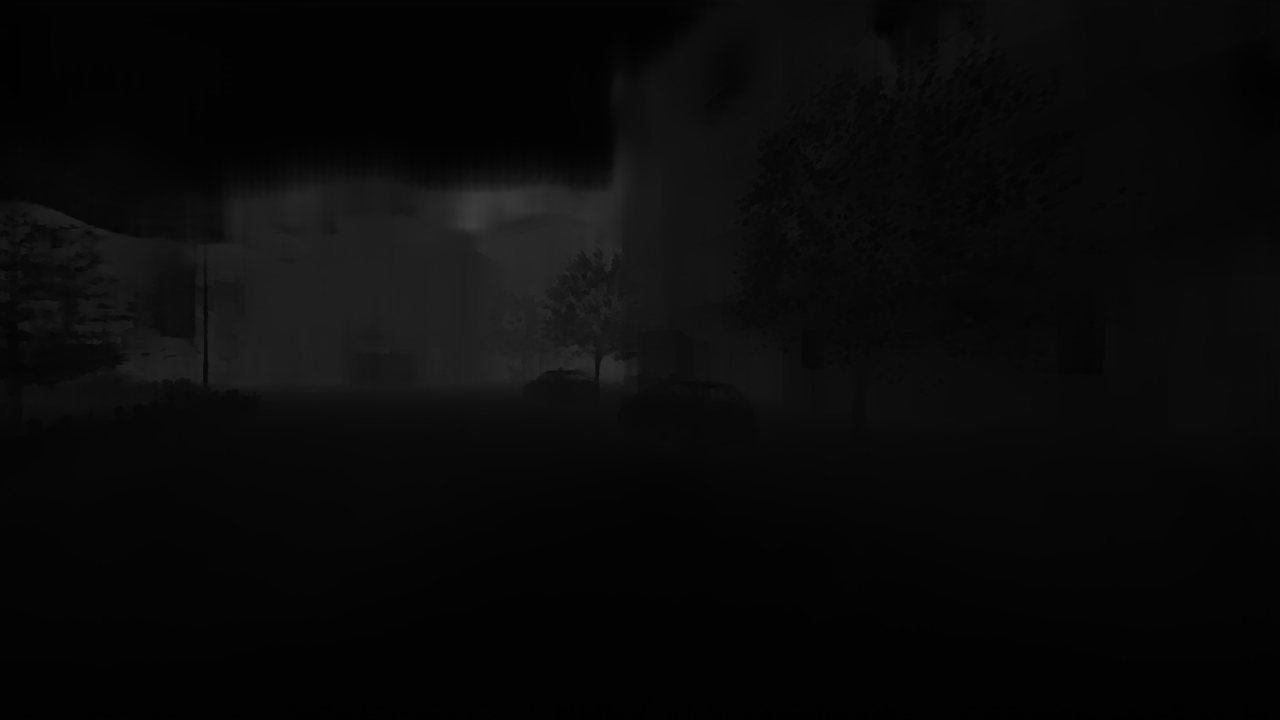
\includegraphics[width=\textwidth]{figures/depth_pred.png}
        \caption{Model output}
        \label{fig:depth_pred}
    \end{subfigure}
    \hfill
    \begin{subfigure}{0.48\textwidth}
        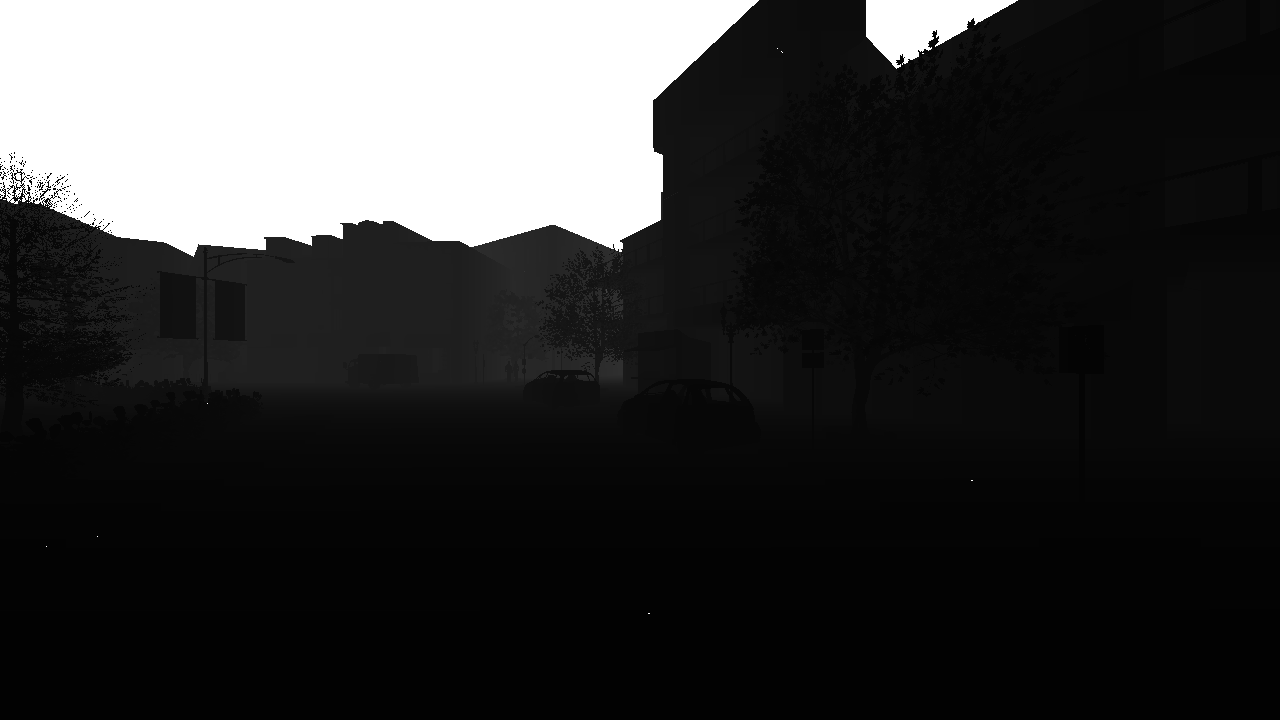
\includegraphics[width=\textwidth]{figures/depth_gt_2.png}
        \caption{Ground truth}
        \label{fig:depth_gt_2}
    \end{subfigure}
    \caption{Depth completion model output compared to ground truth}
    \label{fig:depth_model_comparison}
    \end{figure}


\section{Interface Comparison}

Following the implementation of our three interface variants, we conducted a technical comparison to evaluate their capabilities and performance characteristics. Each interface represents a distinct approach to visualizing teleoperation data:

\subsection*{Separate View}

The Separate View follows the traditional teleoperation interface design principles outlined in Section \ref{section:separateview}. Our implementation enhances the base variant by incorporating \ac{LiDAR} point cloud coloring for improved depth perception and environmental understanding. As shown in Figure \ref{fig:res_sv}, the interface maintains distinct windows for 2D camera feeds and 3D perception data, aligning with established industry approaches like in Figures \ref{fig:Waymo} and \ref{fig:Zoox}.

This variant's key technical advantage lies in its deterministic nature, operating without reliance on deep learning models. The visualization outcome depends solely on direct sensor inputs and rendering processes, making it particularly robust across diverse environments. The absence of learned components provides two significant benefits:
\paragraph{Environmental Adaptability}
The interface maintains consistent performance even in previously unseen scenarios, as it doesn't depend on training data distributions.
\paragraph{View Flexibility}
The point cloud representation maintains accuracy within sensor error bounds when viewed from multiple angles, unlike estimation-based approaches where small errors can compound into visible artifacts during perspective shifts.

These technical characteristics make the Separate View particularly suitable for scenarios requiring high reliability and precise spatial understanding, though at the cost of maintaining multiple display windows.
\begin{figure}[h]
    \centering
    \begin{subfigure}{0.8\textwidth}
        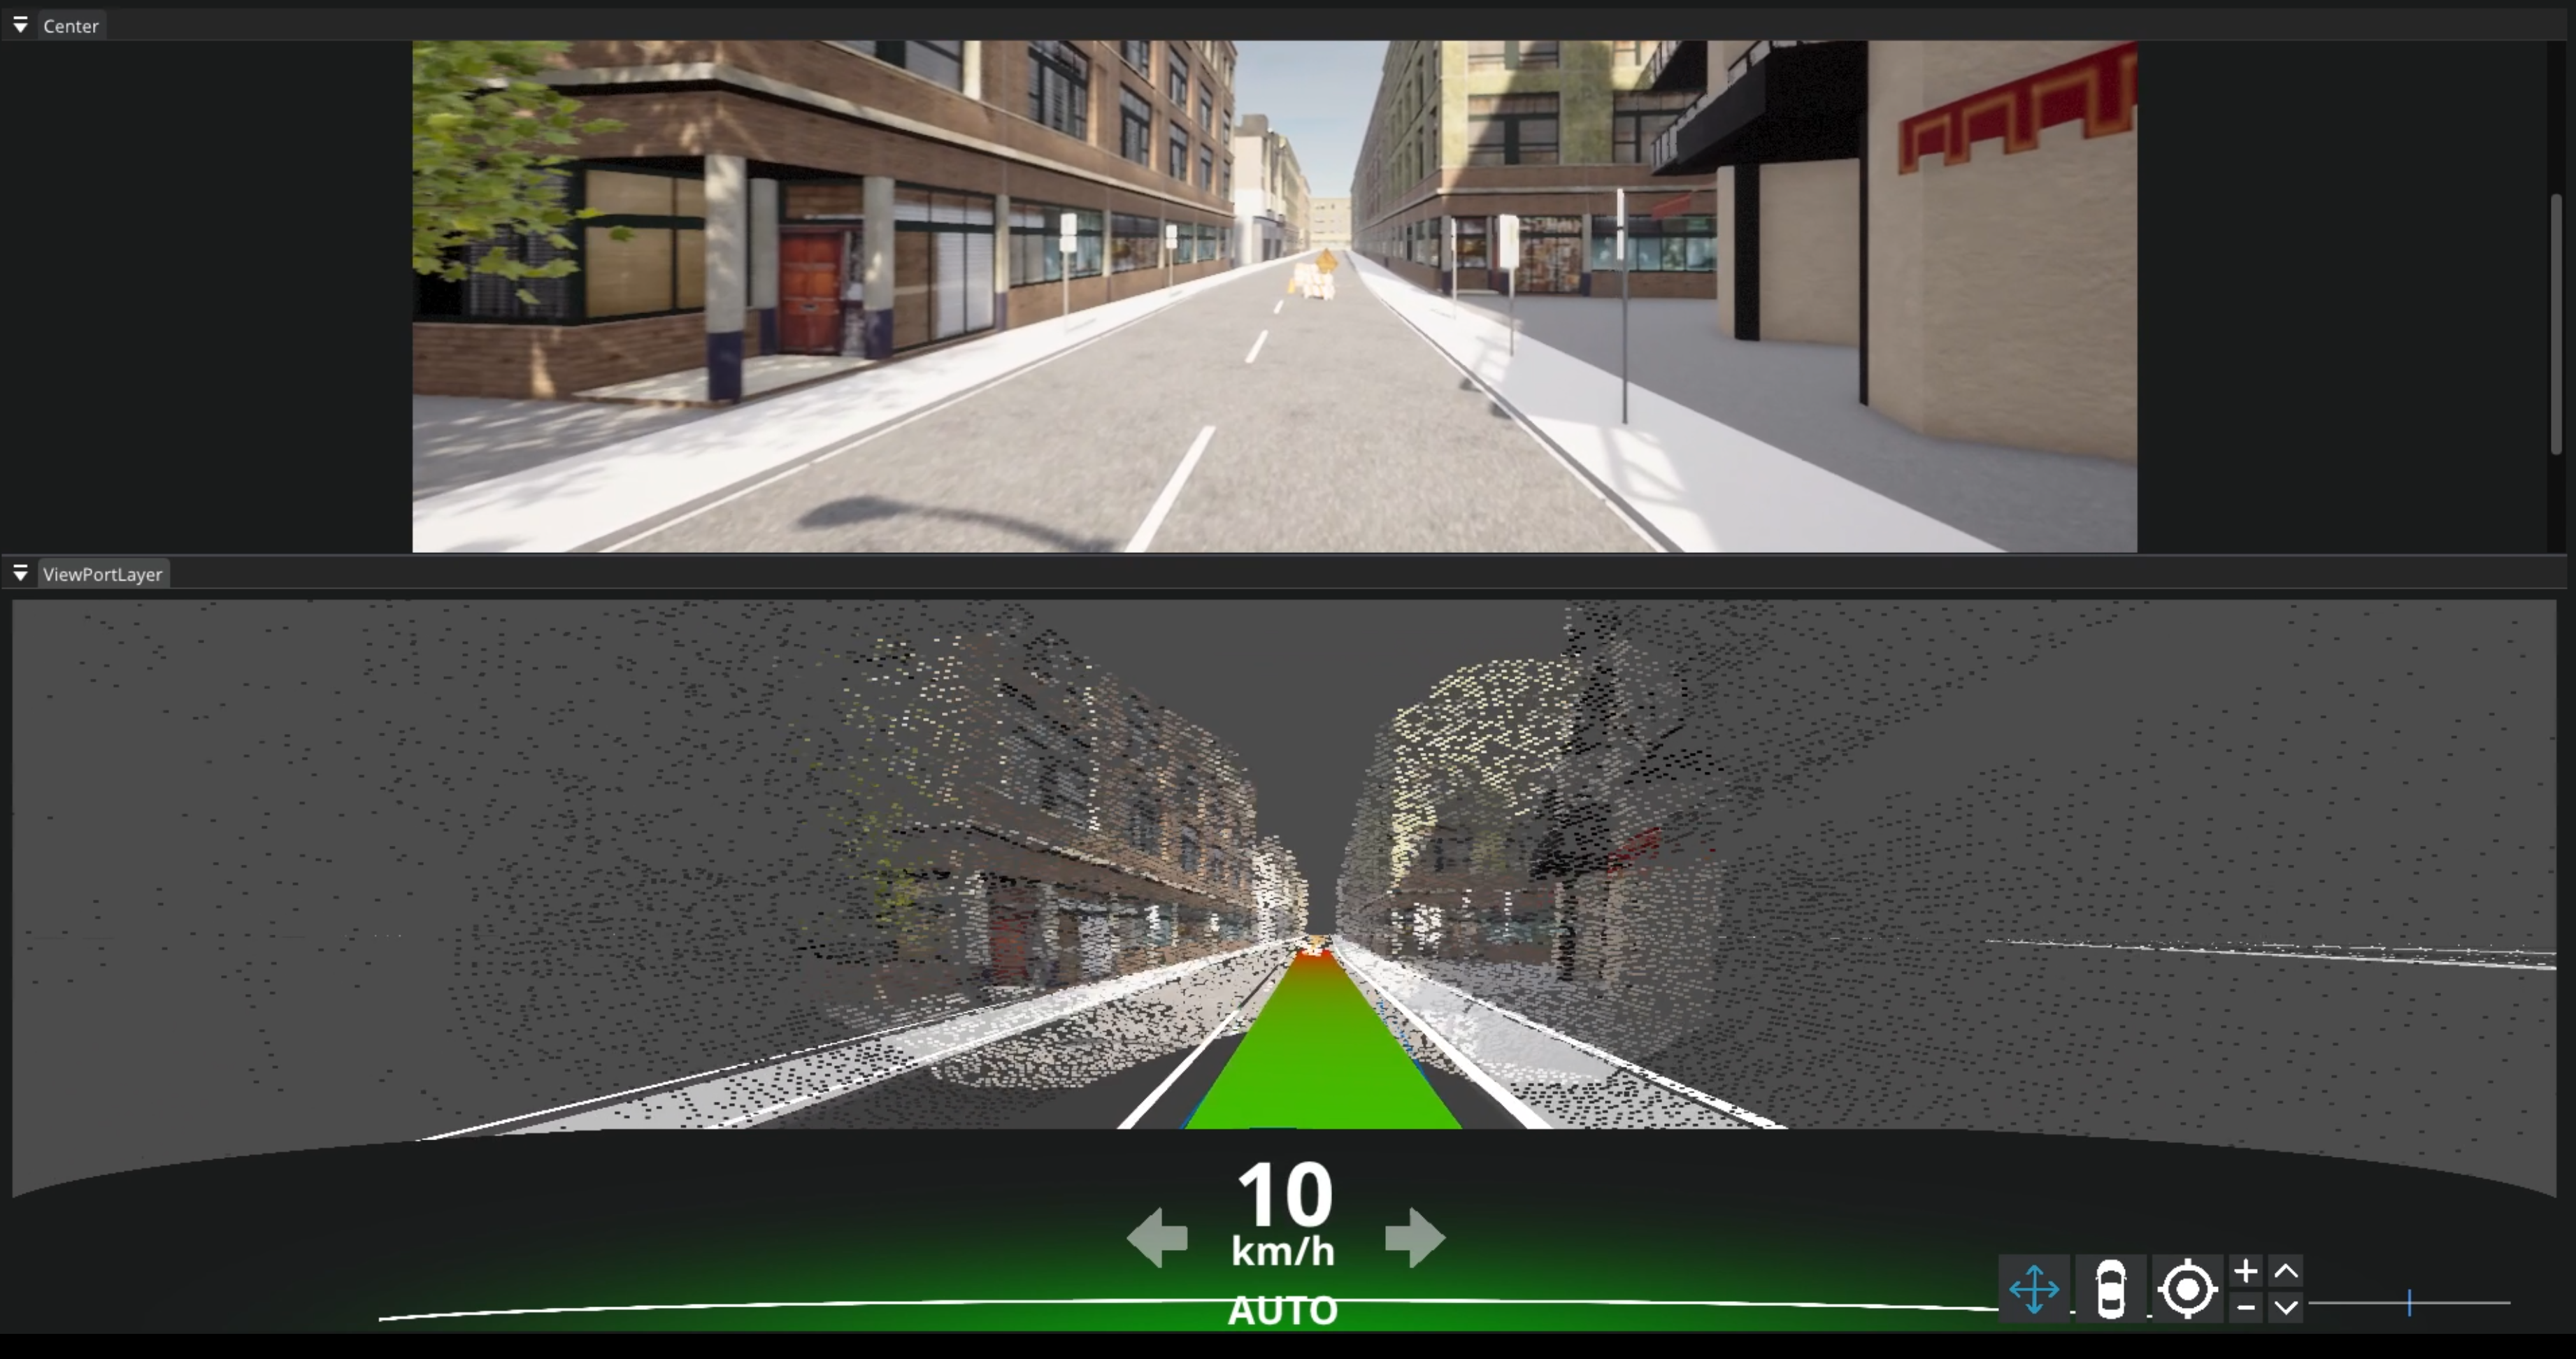
\includegraphics[width=\textwidth]{figures/result_sv.png}
        \centering
        \caption{Separate View Interface before a construction site}
        \label{fig:res_sv_1}
    \end{subfigure}
    \begin{subfigure}{0.8\textwidth}
        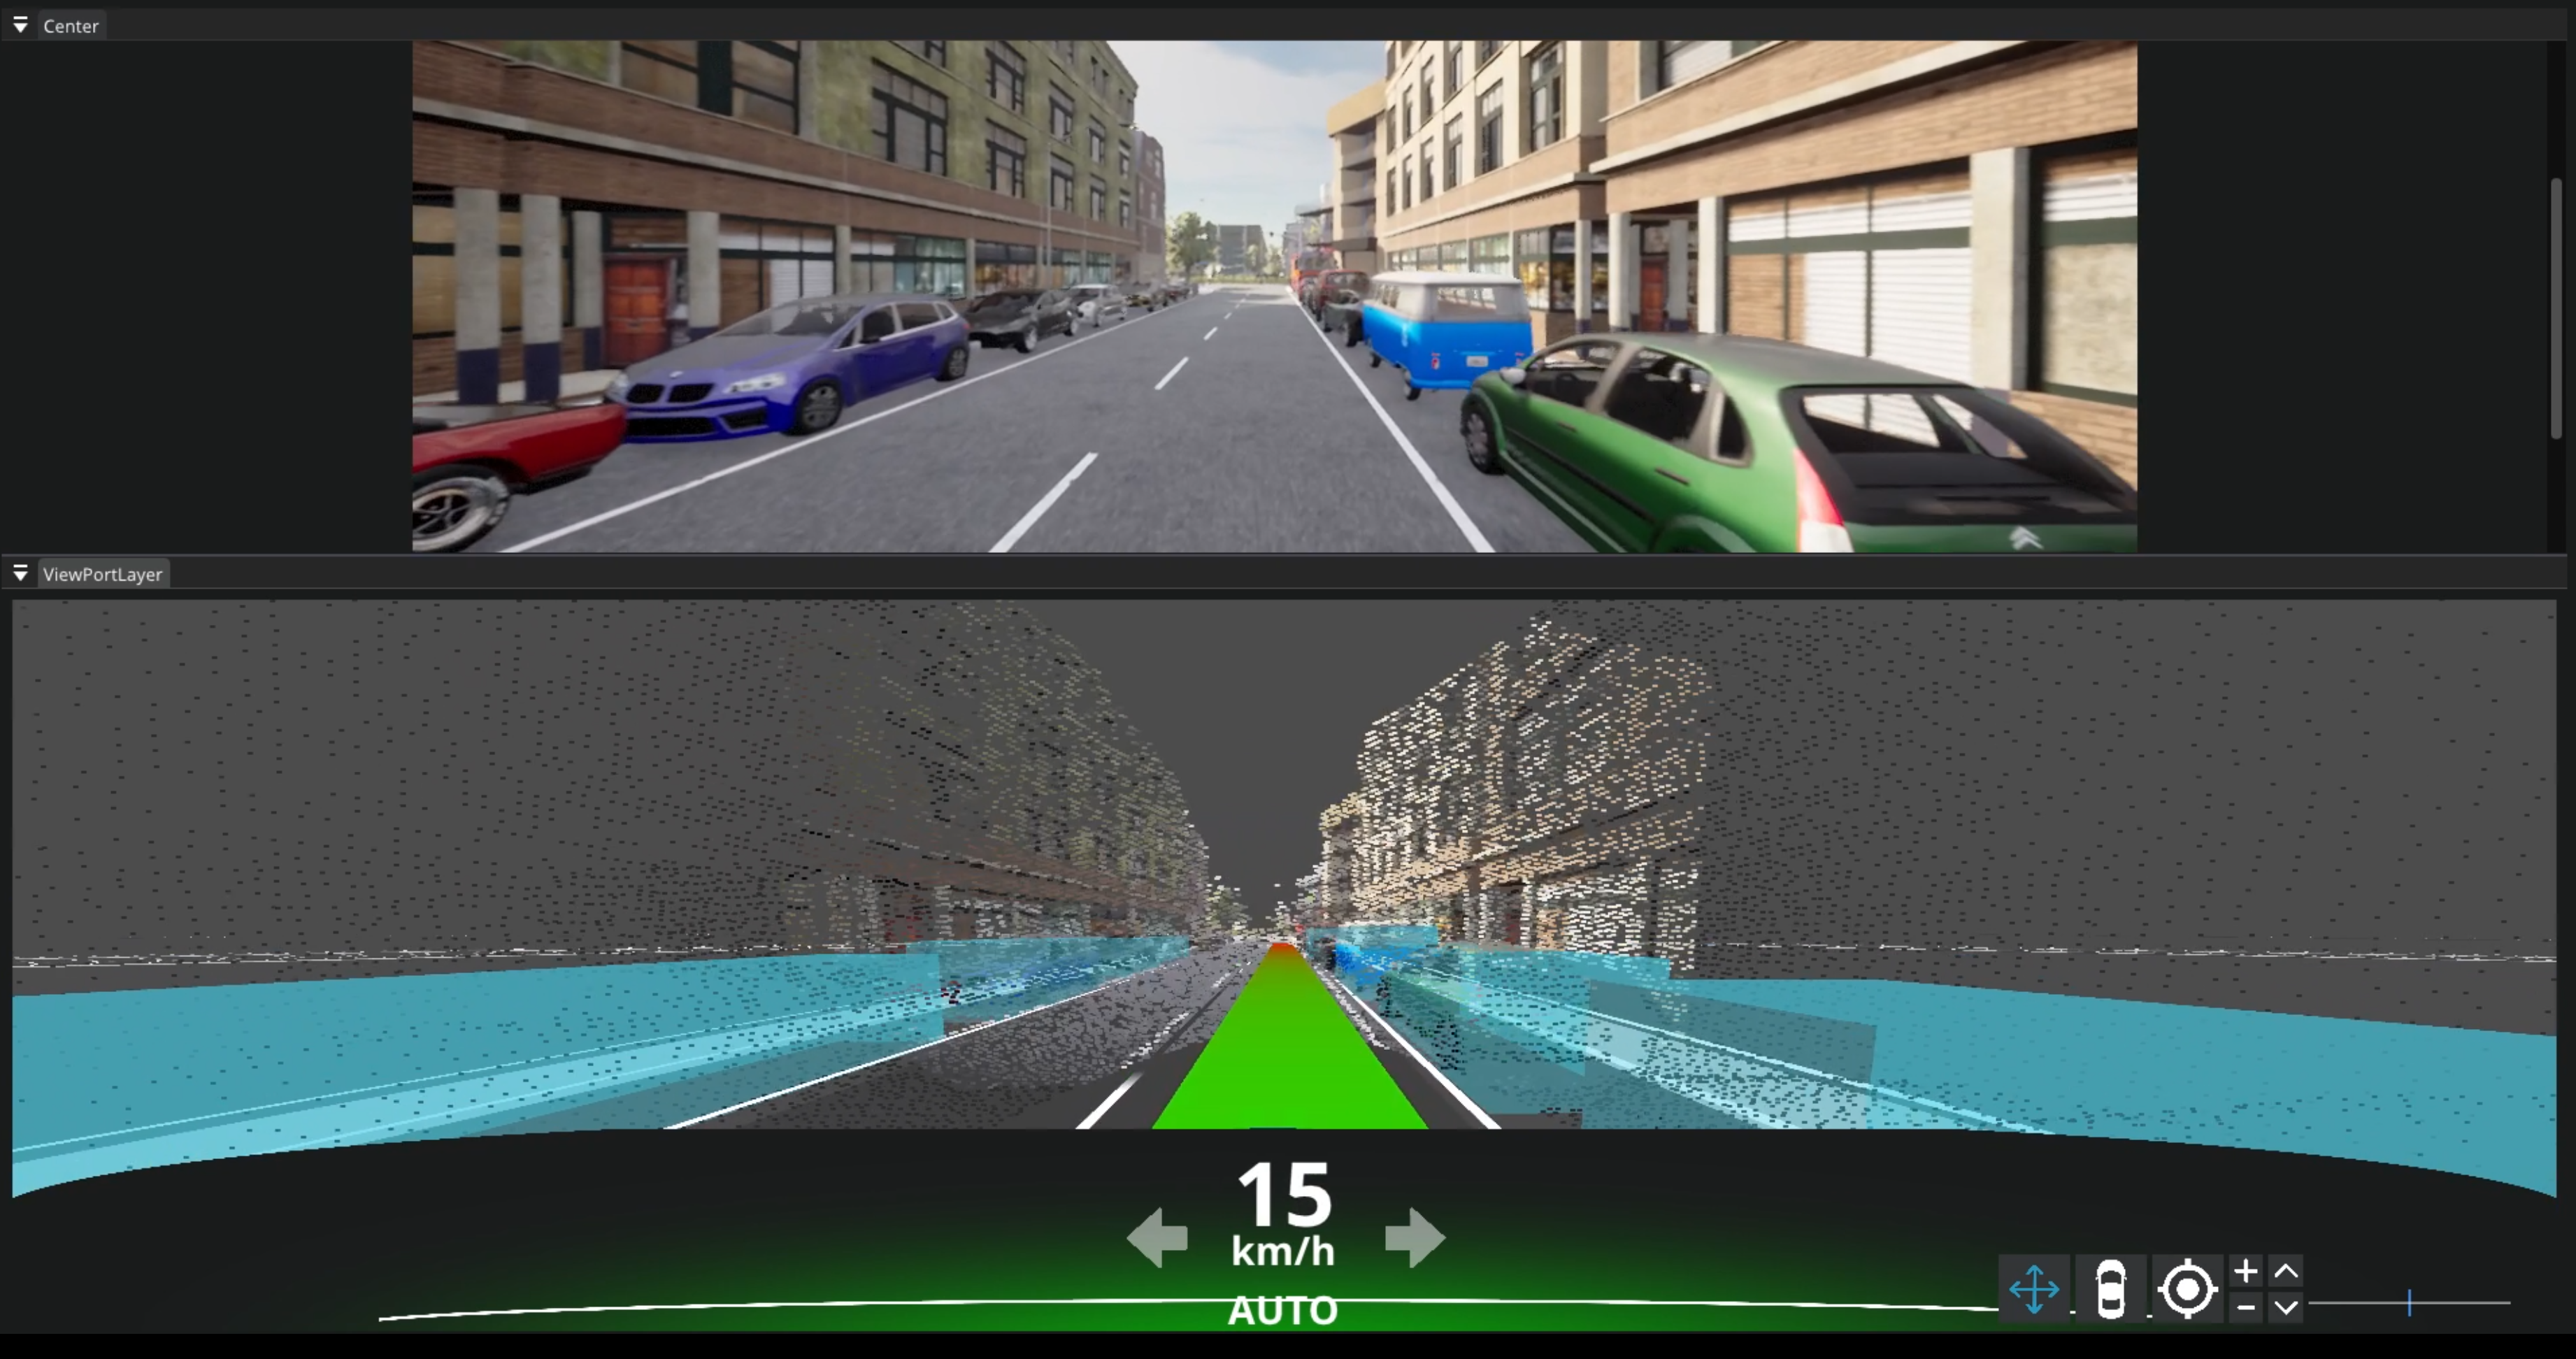
\includegraphics[width=\textwidth]{figures/results_2_sv.png}
        \centering
        \caption{Separate View Interface in a two sided street with parked vehicles}
        \label{fig:res_sv_2}
    \end{subfigure}
    \caption{Separate View Results}
    \label{fig:res_sv}
\end{figure}

\subsection*{Integrated View}

Integrated View is our novel approach to teleoperating interface design defined in the Section \ref{section:integratedview}.
The resulting visualization combining the 2D camera feed and 3D perception data by utilizing a depth completion model can be seen from the Figures \ref{fig:res_iv}.

This variant inherits certain limitations from its reliance on depth completion and training data. The performance notably degrades for environments not well represented in the training dataset. Additionally, as evident in Figure \ref{fig:res_iv_2}, the visualization quality diminishes for objects farther from the ego vehicle, with bounding boxes becoming less distinguishable compared to their representation in the Separate View (Figure \ref{fig:res_sv_2}).

Despite these limitations, the Integrated View offers a significant advantage by consolidating all information into a unified display. This consolidated approach provides an opportunity to evaluate the impact of single-window visualization versus multi-window approaches in teleoperation contexts. The integration of visual data streams into a single coherent view aims to reduce the cognitive load of switching between different displays while maintaining situational awareness.

\begin{figure}[h]
    \centering
    \begin{subfigure}{0.8\textwidth}
        \includegraphics[width=\textwidth]{figures/result_iv.png}
        \centering
        \caption{Integrated View Interface before a construction site}
        \label{fig:res_iv_1}
    \end{subfigure}
    \begin{subfigure}{0.8\textwidth}
        \includegraphics[width=\textwidth]{figures/results_2_iv.png}
        \centering
        \caption{Integrated View Interface in a two sided street with parked vehicles}
        \label{fig:res_iv_2}
    \end{subfigure}
    \caption{Integrated View Results}
    \label{fig:res_iv}
\end{figure}

\subsection*{Integrated View with Ground Truth Depth}
This variant utilizes CARLA's depth camera to obtain perfect depth information for visualization. By using ground truth depth data, it achieves the benefits of the Integrated View's unified visualization approach while avoiding the limitations of depth completion estimation. The interface maintains clear visibility of all objects, including those at greater distances, and provides accurate spatial relationships throughout the entire field of view. Such results can be seen from the Figures \ref{fig:res_gt_1} and \ref{fig:res_gt_2}.

The only technical limitation of this variant is the increased computational overhead due to the dense point-cloud requirements. However, this variant serves purely as a research tool for the user study, establishing an upper bound for visualization quality with perfect depth information. Thus we didn't undergo an in-depth optimization for the rendering process for this variant.

It's important to note that this implementation is not feasible for real-world deployment, as current depth sensing technology cannot provide sufficiently accurate for longer ranges in open environments (Table \ref{table:depth_camera_limitations}). Real-world depth cameras face significant limitations in accuracy and range, particularly under varying lighting conditions. Therefore, this variant primarily serves as a baseline for evaluating the potential of depth completion algorithms and unified visualization approaches.

\begin{figure}[h]
    \centering
    \begin{subfigure}{0.8\textwidth}
        \includegraphics[width=\textwidth]{figures/result_gt.png}
        \centering
        \caption{Integrated View Ground Truth Interface before a construction site}
        \label{fig:res_gt_1}
    \end{subfigure}
    \begin{subfigure}{0.8\textwidth}
        \includegraphics[width=\textwidth]{figures/results_2_gt.png}
        \centering
        \caption{Integrated View Ground Truth Interface in a two sided street with parked vehicles}
        \label{fig:res_gt_2}
    \end{subfigure}
    \caption{Integrated View Ground Truth Results}
    \label{fig:res_gt}
\end{figure}

\paragraph{Performance Analysis}
Runtime performance testing in crowded scenarios revealed significant differences between the three interface variants. The Separate View, processing approximately 18,000 points, achieved the fastest rendering time at 18ms. The Integrated View, despite handling 921,600 points, required 33ms for rendering, while the Ground Truth variant processed around 750,000 points in 52ms.

A detailed analysis of the Separate View's point cloud rendering pipeline revealed three main computational bottlenecks:

- Coordinate system transformation: 3ms

- Image plane projection: 5ms

- Adding points to the mesh and cropping: 5ms

The modular design of the Ground Truth and Separate View renderers performs these operations sequentially. In contrast, the \emph{Integrated View} Renderer benefits from first, having a depth image in the camera space, means it doesn't need some of the costly steps like coordinate system transformation and image plane projection. Those steps are handled within the model, and the model runs it's estimation's on parallel as defined in the Section \ref{section:performanceoptimization}
This optimization strategy proves highly effective, as the \emph{Integrated View} processes over fifty times more points than the Separate View while only requiring an additional 15ms of processing time.

\begin{table}[h!]
\centering
\begin{tabular}{|p{3.5cm}|p{3cm}|p{3cm}|p{3cm}|}
\hline
\textbf{Feature} & \textbf{Separate View} & \textbf{Integrated View} & \textbf{Integrated View GT} \\
\hline
Processing Time & 18ms & 33ms & 52ms \\
\hline
Point Cloud Size & ~18k points & 921.6k points & ~750k points \\
\hline
Update Frequency & Real-time & Near real-time & Real-time \\
\hline
\end{tabular}
\caption{Performance comparison of interface variants}
\label{table:interface_comparison}
\end{table}

It's important to note that these measurements focus solely on the point cloud rendering pipeline, excluding the parallel depth estimation process in the Integrated View. The performance metrics demonstrate that our optimization strategies successfully manage the increased computational demands of processing larger point clouds while maintaining acceptable runtime performance.

% !TeX root = ../main.tex
% Add the above to each chapter to make compiling the PDF easier in some editors.

\chapter{Discussion}\label{chapter:discussion}

\section{Interpretation of Results}

\section{Limitations of the Method}
% !TeX root = ../main.tex
% Add the above to each chapter to make compiling the PDF easier in some editors.

\chapter{Conclusion}\label{chapter:conclusion}

This chapter concludes the thesis by summarizing the main contributions, discussing limitations in the applied methodology, and outlining potential future research directions for teleoperation interface designs targeting \ac{AV} use cases. The findings and developments presented in this work lay a foundation for advancing the Perception Modification concept in \acp{AV}, aiming to enhance operators' situational awareness and overall teleoperation performance.

\section{Summary of Contribution}
This thesis focused on designing, implementing, and planning an evaluation of two distinct teleoperation \ac{HMI} approaches to support Perception Modification tasks for \acp{AV}. Several key contributions were made:

    \textbf{Requirements and Literature Synthesis:} Through a comprehensive review in Chapter \ref{chapter:literaturereview}, the thesis outlined the evolving landscape of \acp{AV} and teleoperation, emphasizing \ac{SA}, cognitive workload, and user acceptance as core design objectives. These insights led to a defined set of system-level and interface-level requirements that guided the subsequent development (see \ref{table:requirements}).

    \textbf{Two Interface Designs:}
    In Chapter \ref{chapter:methodology}, two teleoperation interface approaches were developed atop the ToD Visual 2.0 framework. The \emph{Separate View} (\ref{section:separateview}) keeps raw camera feeds and 3D perception data on separate displays, following existing industry conventions. In contrast, the \emph{Integrated View} (\ref{section:integratedview}) unifies raw sensor data and perception outputs in a single window, aiming to reduce cognitive load from switching between multiple views.

    \textbf{Depth Completion for Unified Visualization:}  To enable the Integrated View, a \ac{DL} depth completion pipeline was constructed (see \ref{section:integratedviewimplementation}). While its performance was not state-of-the-art compared to specialized depth completion benchmarks, it delivered sufficiently dense 3D information to investigate whether unified rendering improves operator \ac{SA} and teleoperation performance.

    \textbf{User Study Development:}
    A comprehensive user study design in Chapter \ref{chapter:userstudy} was established, featuring scenario creation, questionnaire structures (\ac{SAGAT}, \ac{NASA-TLX}), and a custom simulation environment based on Munich’s Gärtnerplatz. This framework allows direct comparisons among the Separate View, the Integrated View, and an Integrated View with ground-truth depth as a baseline reference.


Together, these elements form a cohesive approach to exploring how different visualization strategies influence operator effectiveness in teleoperating \acp{AV} for Perception Modification tasks. The results in Chapter \ref{chapter:results} highlight technical comparisons and demonstrate the feasibility of each interface variant, setting the stage for extensive user evaluations in future work.

\section{Limitations of the Methodology}

Several constraints and challenges arose during the research process that may influence the generalizability and interpretation of the findings:

    \textbf{Simulation-oriented Method:} All implementation and scenario testing took place within the CARLA simulator integrated with Autoware. Although this setup provides repeatable scenarios and precise ground-truth data, real-world complexities (e.g., lighting variations, sensor noise, network inconsistencies) were not directly addressed. They are in some level simulated with the help of the CARLA simulator with different weather conditions and lighting settings, but the realism of the simulation is still limited.

    \textbf{Depth Completion Generalization:}
    The depth completion model was trained on a specific simulated dataset and showed decreased accuracy for objects at longer ranges. Extending to real-world conditions would require substantially more diverse training sets and additional validation against real sensor data.

    \textbf{Limited Real-time Evaluation:}
    The thesis focused on developing the user study structure (\ref{chapter:userstudy}) rather than fully executing it. While extensive scenario creation and technical preparations were completed, user tests and statistical analyses of their \ac{SA} or workload remain for subsequent research.

    \textbf{Network Considerations:}
    Although communication bandwidth and latency were recognized as critical in teleoperation (\ref{section:challenges}), the interfaces were not stress-tested under extreme or unreliable network conditions. Practical deployment would likely require further optimizations to meet real-world throughput and latency constraints.

    \textbf{Implementation Trade-offs:}
    Certain design decisions—such as focusing on a single forward-facing camera with a specific field of view—reflected practical engineering choices more than exhaustive design optimization. Incorporating wider camera coverage or multi-camera depth fusion could further improve operator \ac{SA}.

\section{Future Research Directions}

Based on insights gained from this thesis, several prominent directions would extend and refine the work:

\textbf{Empirical User Study Execution:}
Conducting the planned user study (\ref{chapter:userstudy}) with a representative group of participants is a key next step to empirically compare the Separate View and Integrated View in terms of \ac{SA}, mental workload, and operator performance. This data-driven validation is essential for confirming the hypothesized benefits of unified visualization.

\textbf{Enhanced 3D Reconstruction Techniques:}
Further research could explore alternative methods—such as \ac{NeRF} or improved self-supervised depth completion—to yield more robust, higher-fidelity 3D reconstructions. Understanding how improved depth reconstruction affects operators’ teleoperation performance is an open question, especially in complex or dynamic scenes.

\textbf{Broadening Teleoperation Concepts:}
The Perception Modification concept could be tested alongside other teleoperation approaches (e.g., Shared Control, Remote Driving) to discern whether a unified view also benefits tasks requiring direct vehicle control or collaborative path planning. Exploring multi-modal cue integration (e.g., haptic feedback) may further enrich operator awareness.

\textbf{Full Perception Modification:}
Integrating the Perception Modification interface with real-time sensor data modification capabilities (e.g., object removal, lane marking adjustment) would enable operators to actively manipulate the environment. Evaluating the effectiveness of these modifications on operator \ac{SA} and task performance is a promising avenue for future research.

\textbf{Real-world Prototyping:}
Future work might integrate the developed interfaces with actual sensor feeds on research vehicles like the TUM EDGAR. This real-world testing could illuminate issues hidden in simulation—such as varying sensor latencies, occlusions, or multi-sensor calibration challenges—and refine data transmission protocols under realistic network environments.

\textbf{Multi-vehicle Teleoperation and Scalability:}
Scaling teleoperation to fleets of \acp{AV} requires user interfaces capable of monitoring and intervening in multiple vehicles concurrently. Research could investigate strategies for dynamically prioritizing operator attention, partitioning interface layouts for multi-stream data, or automating routine Perception Modifications.

In conclusion, this thesis contributes toward more advanced \ac{HMI} solutions, specifically targeting Perception Modification scenarios for \acp{AV}. By comparing and contrasting a well-established Separate View approach with a novel Integrated View concept, the research clarifies the technological and human-factor trade-offs inherent in teleoperation interfaces. Although definitive user-results lie beyond the current scope, the groundwork and design blueprint provided here will enable more systematic evaluations, ultimately guiding the design of next-generation teleoperation systems that enhance safety, efficiency, and public acceptance of \acp{AV}.
% TODO: add more chapters here

\appendix{}

\microtypesetup{protrusion=false}
\listoffigures{}
\listoftables{}
\microtypesetup{protrusion=true}
\printbibliography{}

\end{document}
